\chapter{Casos de Uso}

\section{Fazer envio de uma única foto}

\subsection{HTA Model}

\begin{figure}[H]
    \centering
    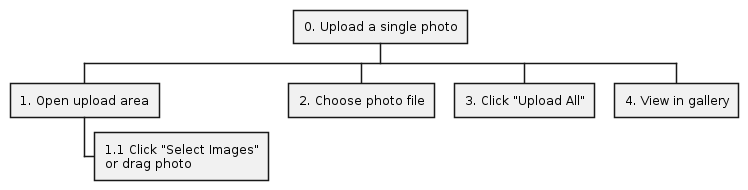
\includegraphics[width=0.9\textwidth]{../figures/hta/UC001.png}
    \caption{HTA Model para o caso de uso: Envio de uma única foto. Fonte: os autores}
    \label{fig:hta-uc001}
\end{figure}

\subsection{Diagrama de Sequência}

\begin{figure}[H]
    \centering
    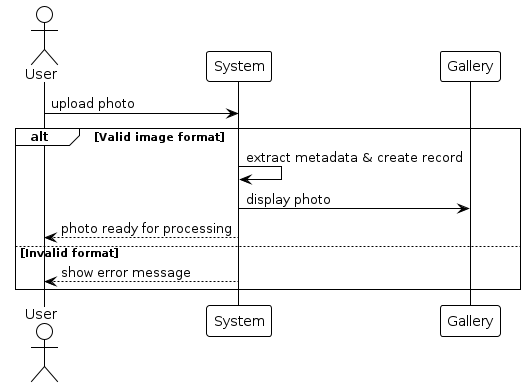
\includegraphics[width=0.9\textwidth]{../figures/dss/UC001.png}
    \caption{Diagrama de sequência para o caso de uso: Envio de uma única foto. Fonte: os autores}
    \label{fig:dss-uc001}
\end{figure}

\subsection{Telas da Aplicação}

\begin{figure}[H]
    \centering
    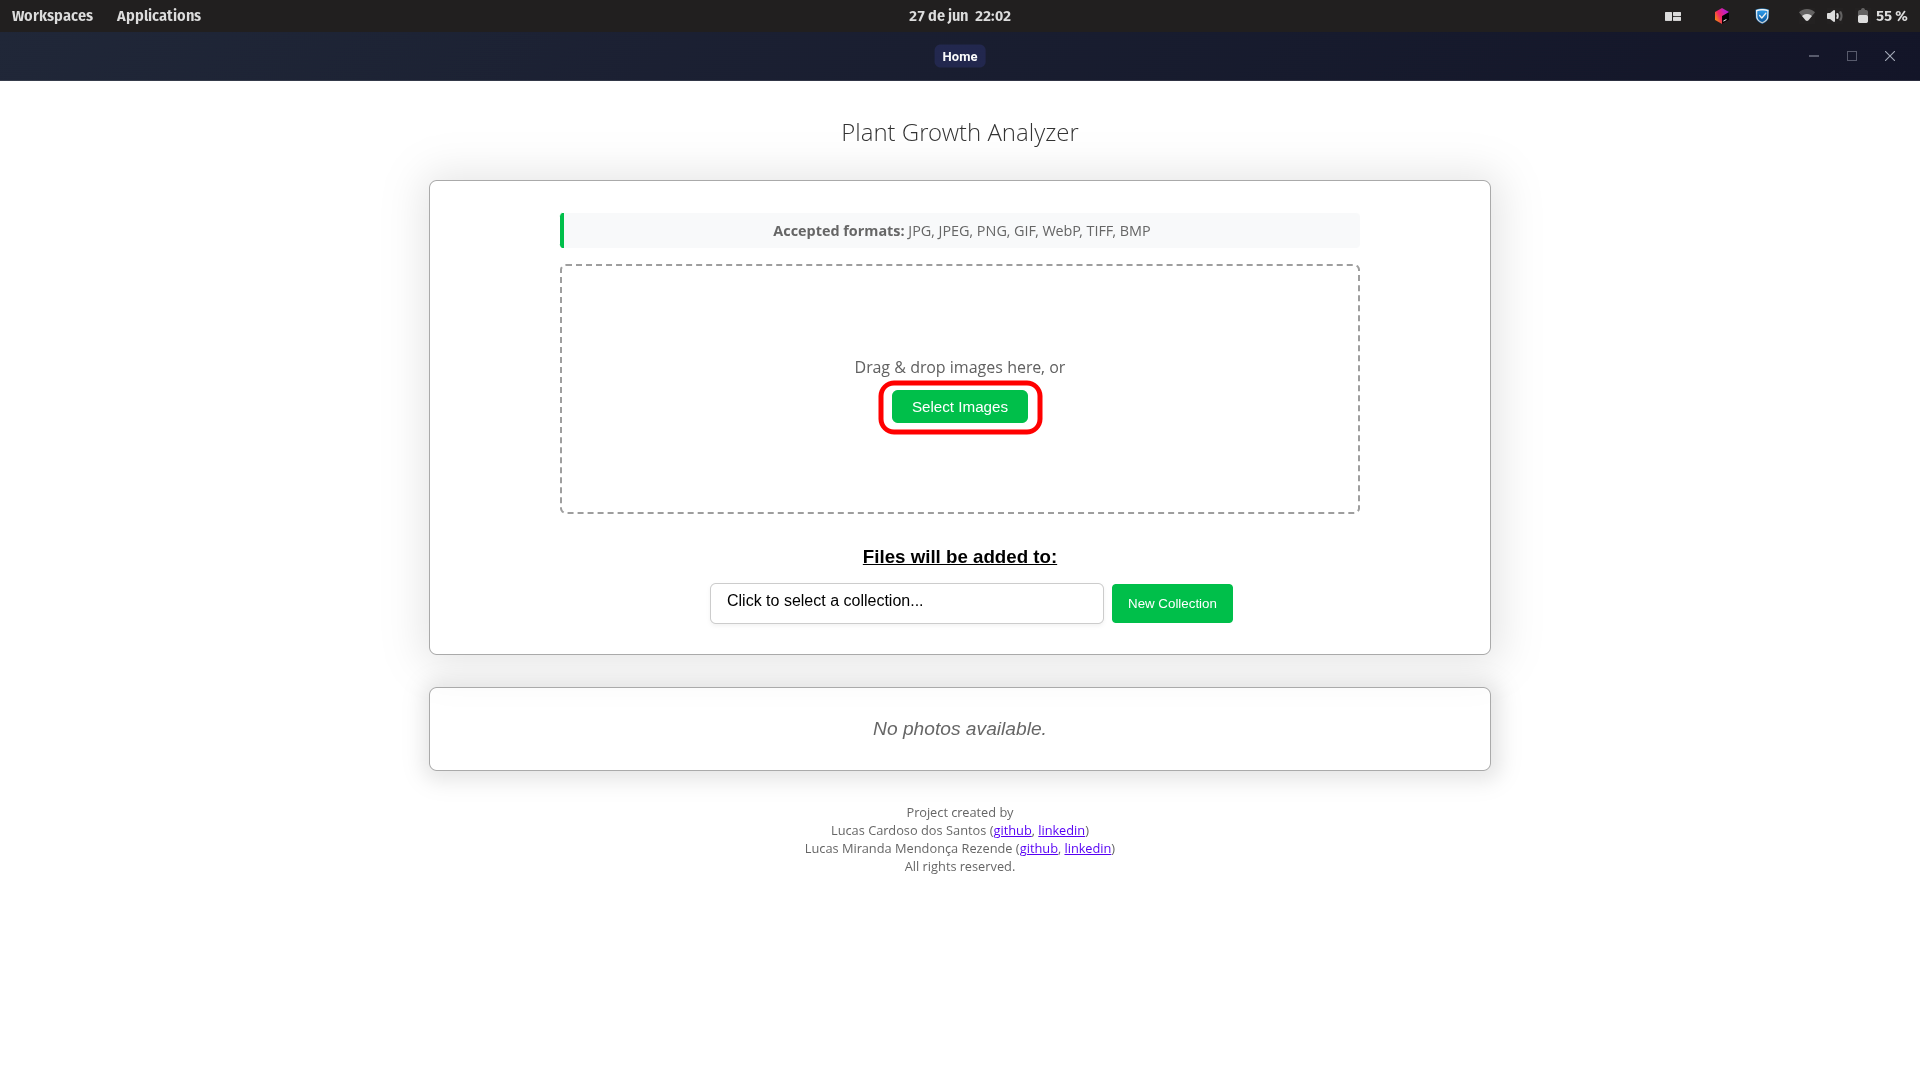
\includegraphics[width=1\textwidth]{../figures/screens/uc001/Screenshot from 2025-06-27 22-02-51.png}
    \caption{Tela inicial da aplicação. Fonte: os autores}
    \label{fig:uc001-screen1}
\end{figure}

\begin{figure}[H]
    \centering
    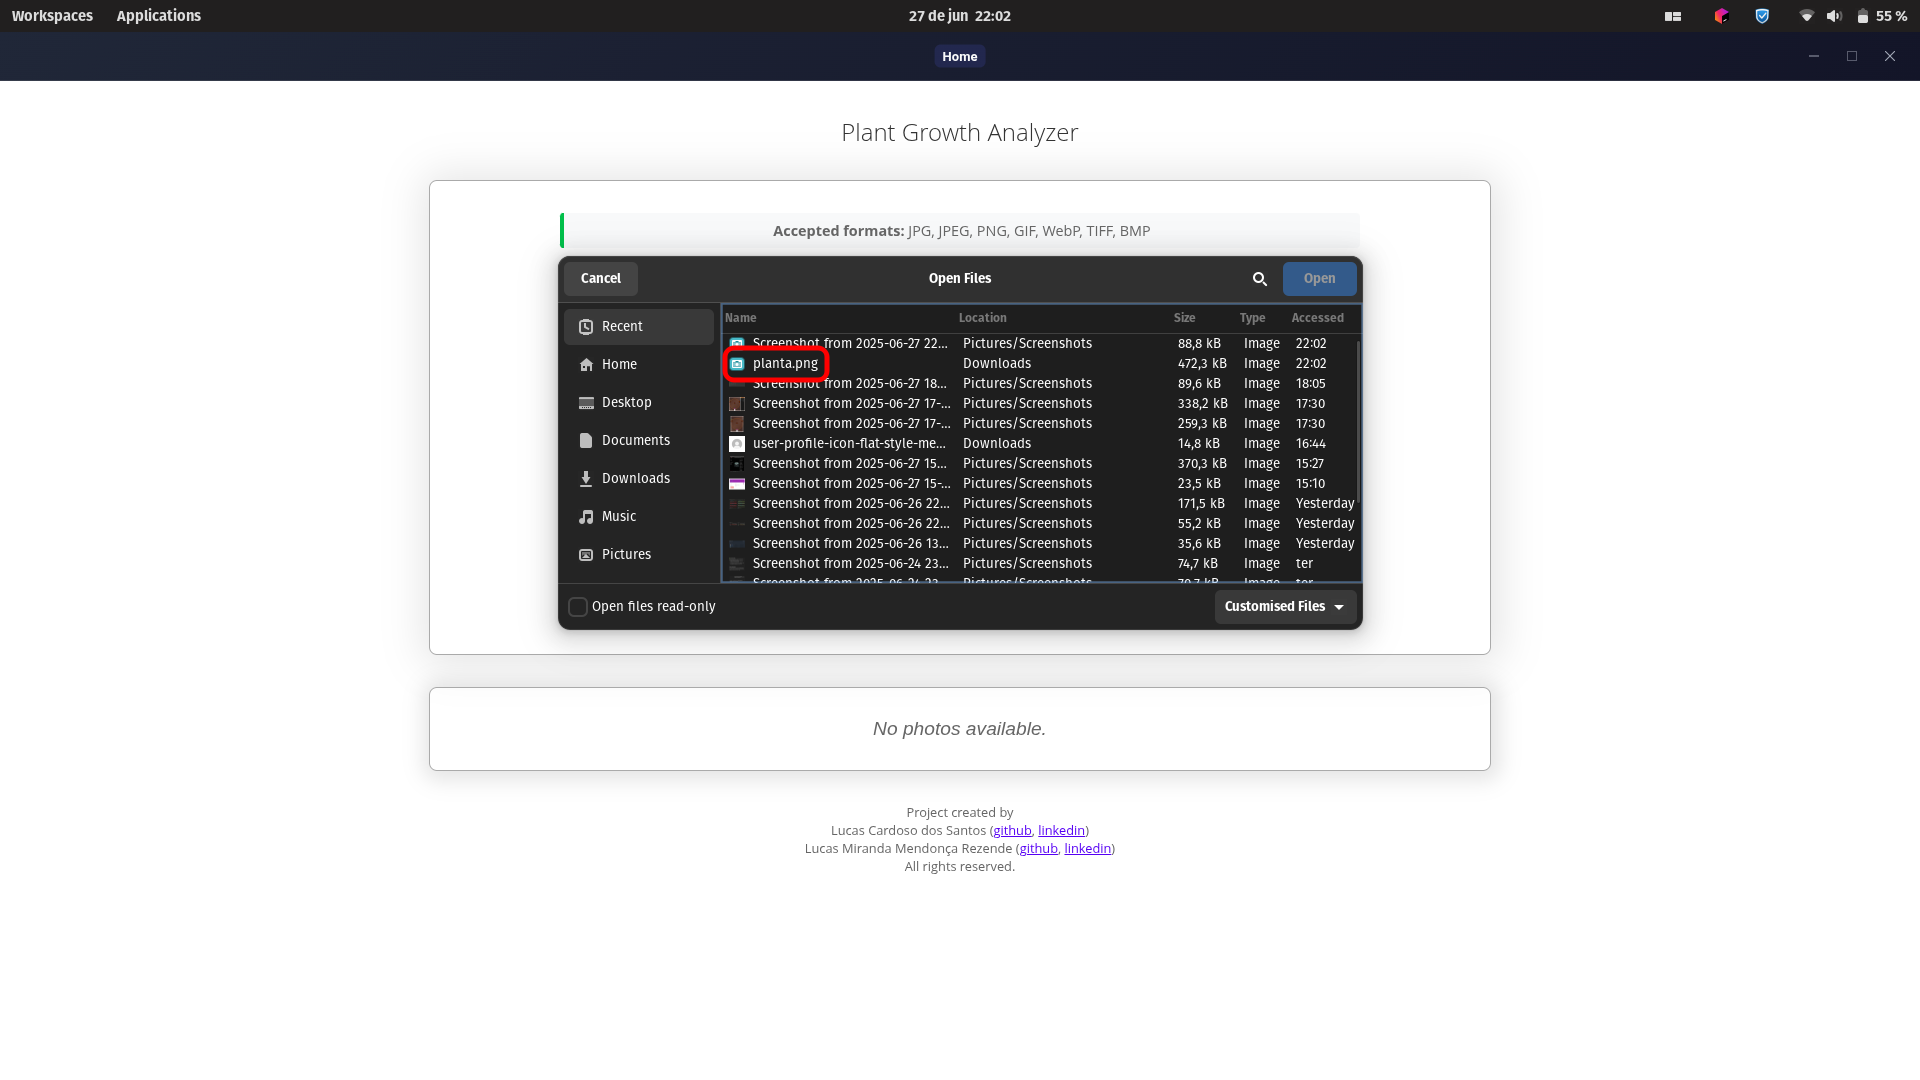
\includegraphics[width=1\textwidth]{../figures/screens/uc001/Screenshot from 2025-06-27 22-02-56.png}
    \caption{Seleção de arquivo para upload. Fonte: os autores}
    \label{fig:uc001-screen2}
\end{figure}

\begin{figure}[H]
    \centering
    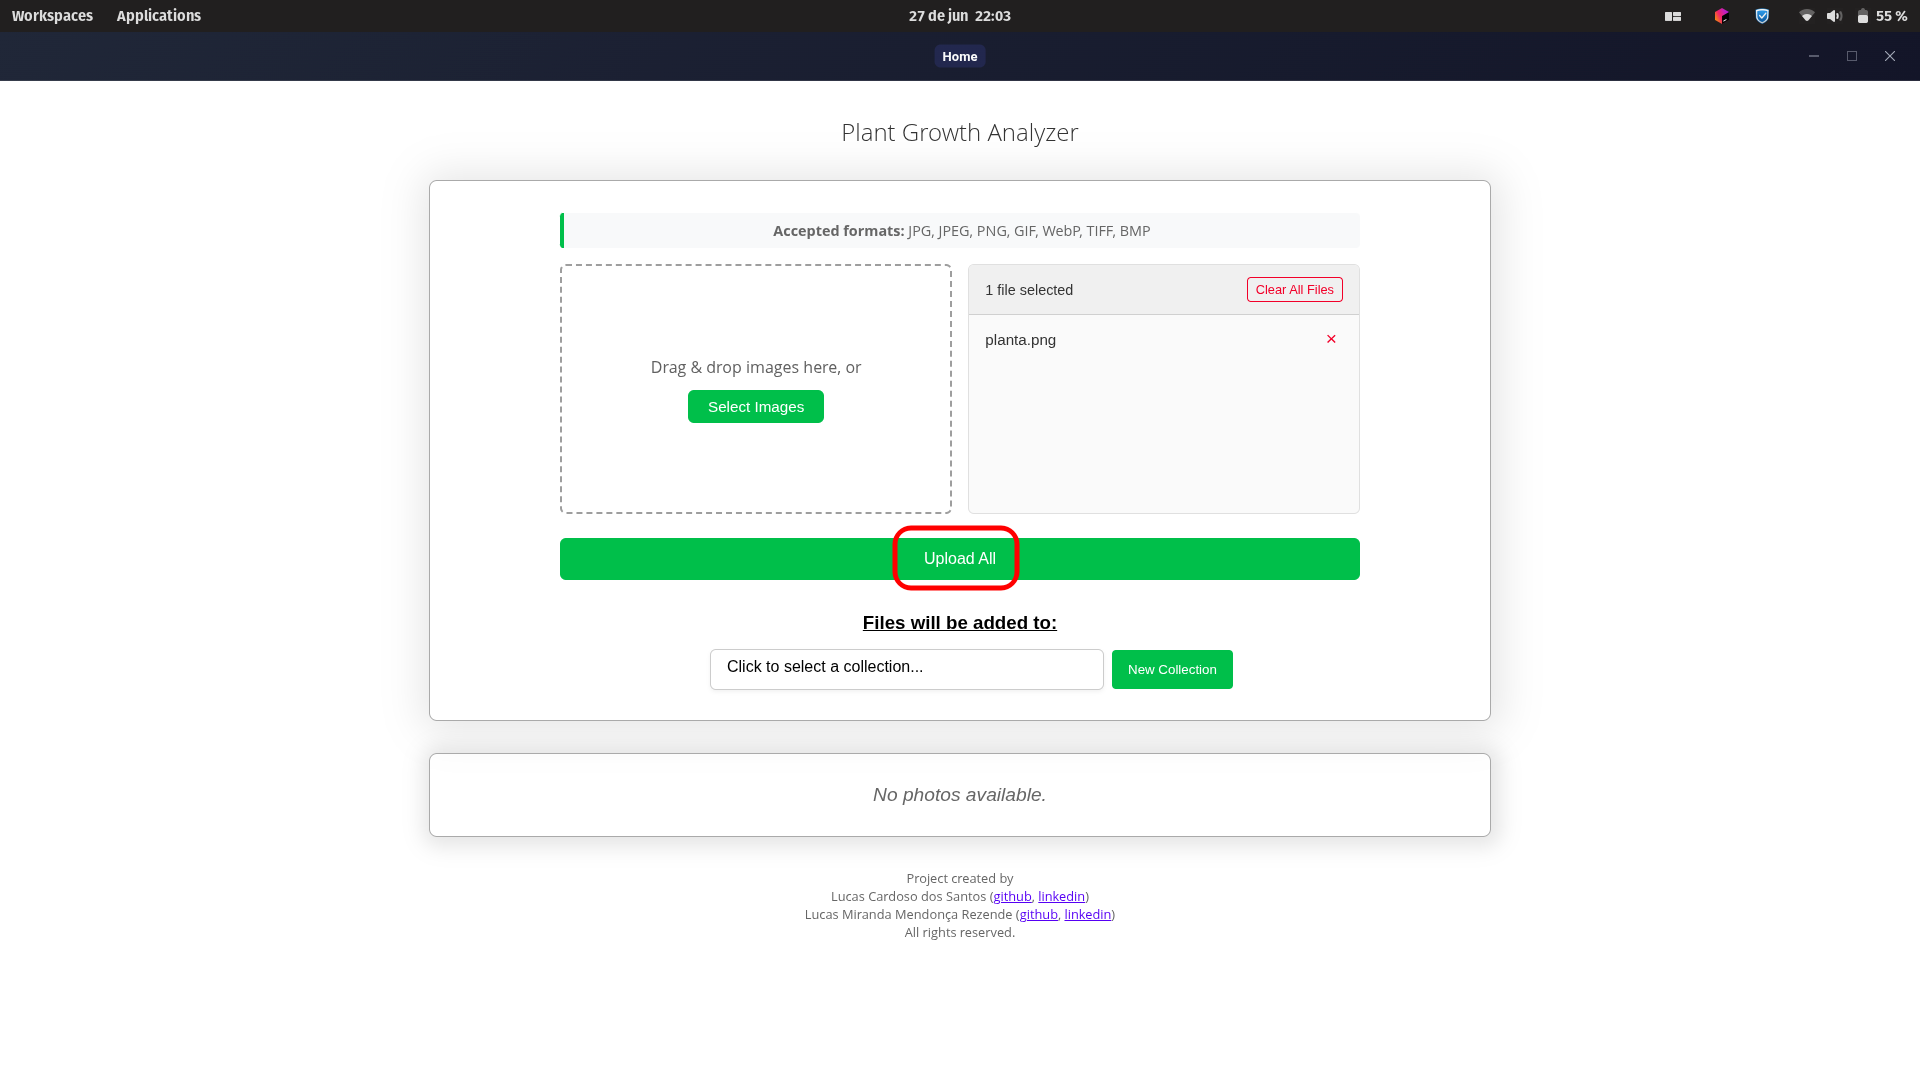
\includegraphics[width=1\textwidth]{../figures/screens/uc001/Screenshot from 2025-06-27 22-03-05.png}
    \caption{Envio da imagem selecionada. Fonte: os autores}
    \label{fig:uc001-screen3}
\end{figure}

\begin{figure}[H]
    \centering
    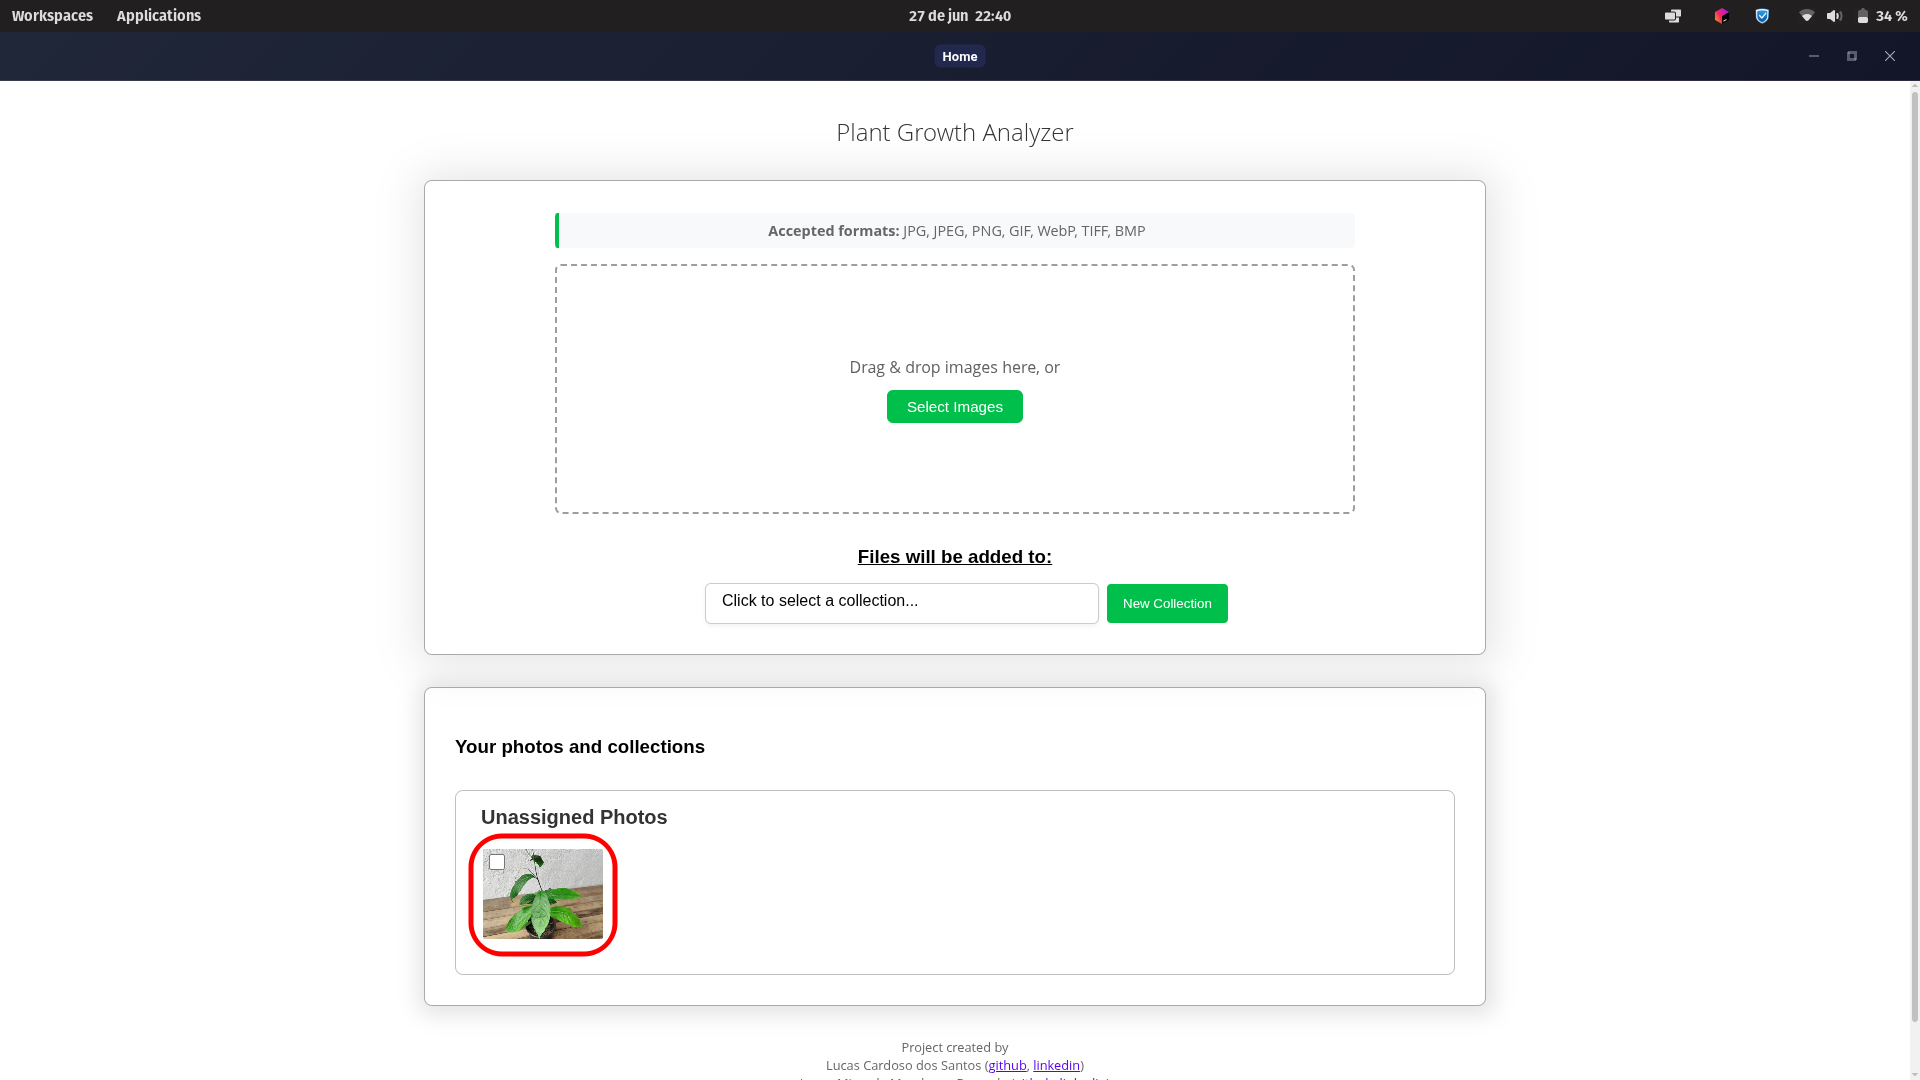
\includegraphics[width=1\textwidth]{../figures/screens/uc001/Screenshot from 2025-06-27 22-03-20.png}
    \caption{Imagem salva. Fonte: os autores}
    \label{fig:uc001-screen4}
\end{figure}

\section{Fazer envio de múltiplas imagens}

\subsection{HTA Model}

\begin{figure}[H]
    \centering
    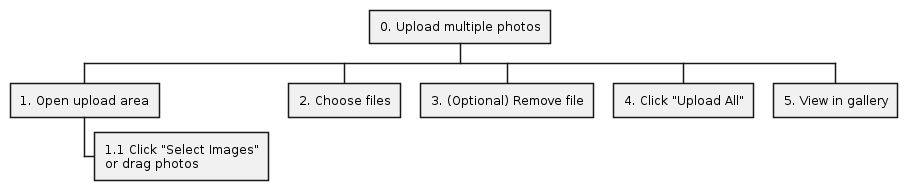
\includegraphics[width=0.9\textwidth]{../figures/hta/UC002.png}
    \caption{HTA Model para o caso de uso: Envio de múltiplas imagens. Fonte: os autores}
    \label{fig:hta-uc002}
\end{figure}

\subsection{Diagrama de Sequência}

\begin{figure}[H]
    \centering
    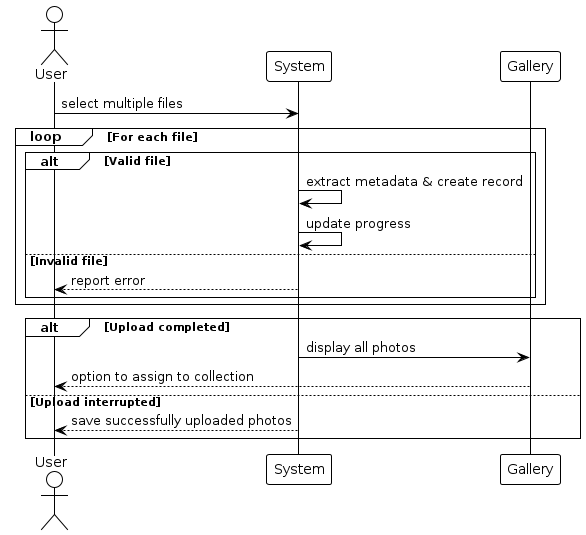
\includegraphics[width=0.9\textwidth]{../figures/dss/UC002.png}
    \caption{Diagrama de sequência para o caso de uso: Envio de múltiplas imagens. Fonte: os autores}
    \label{fig:dss-uc002}
\end{figure}

\subsection{Telas da Aplicação}

\begin{figure}[H]
    \centering
    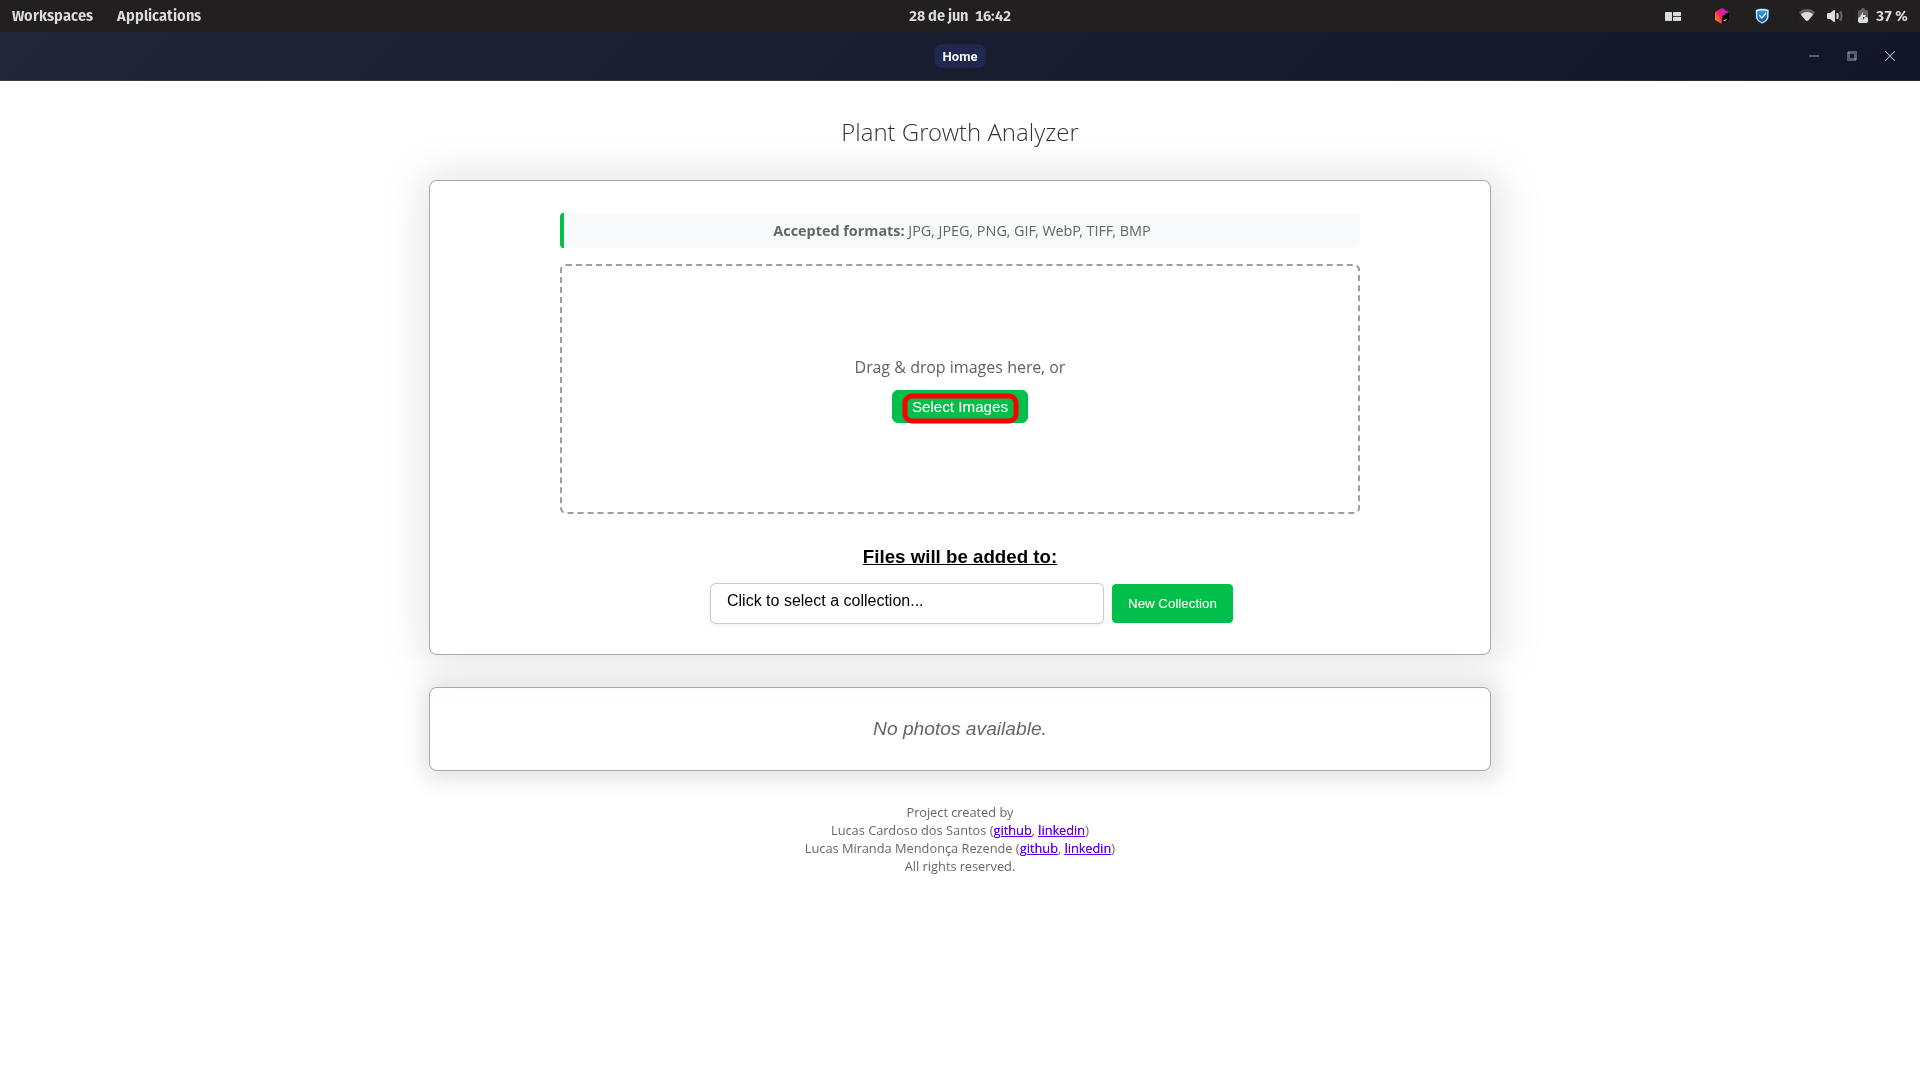
\includegraphics[width=1\textwidth]{../figures/screens/uc002/Screenshot from 2025-06-28 16-42-44.png}
    \caption{Tela inicial para upload múltiplo. Fonte: os autores}
    \label{fig:uc002-screen1}
\end{figure}

\begin{figure}[H]
    \centering
    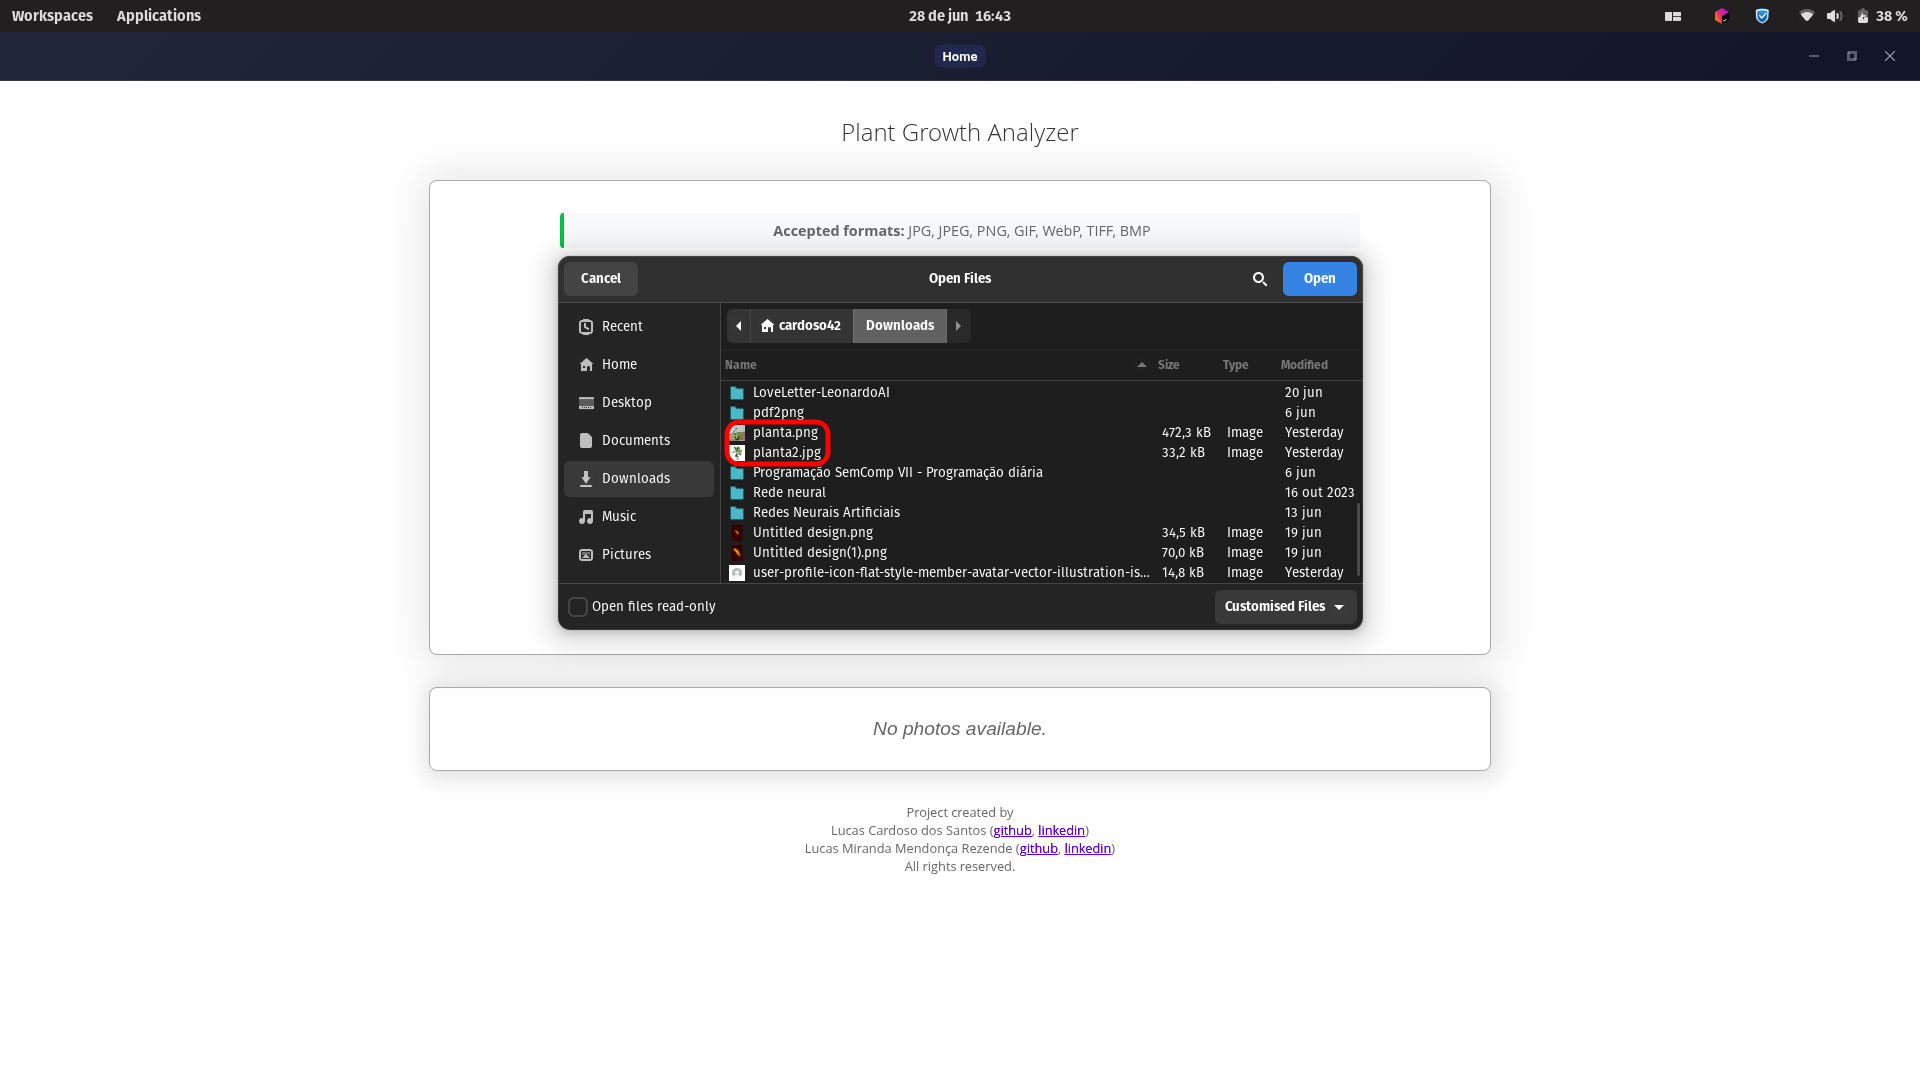
\includegraphics[width=1\textwidth]{../figures/screens/uc002/Screenshot from 2025-06-28 16-43-08.png}
    \caption{Seleção de múltiplos arquivos. Fonte: os autores}
    \label{fig:uc002-screen2}
\end{figure}

\begin{figure}[H]
    \centering
    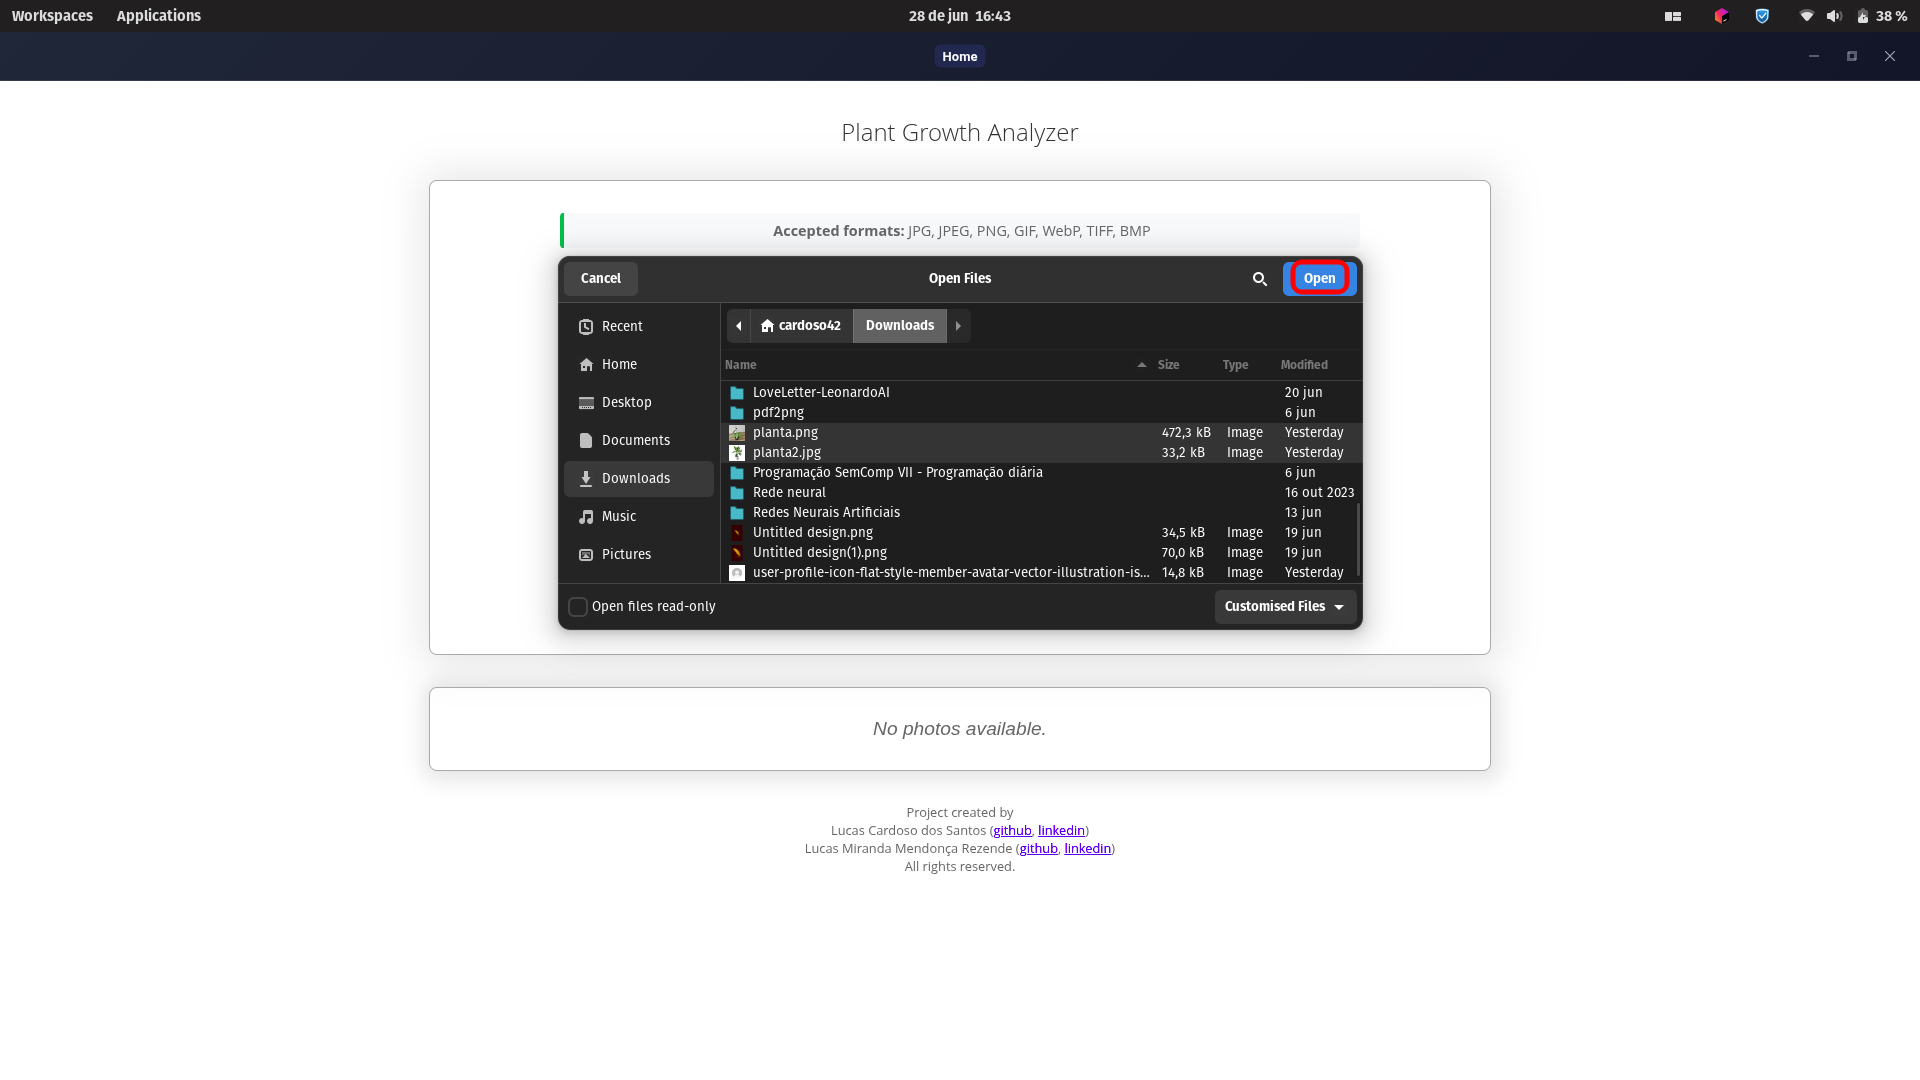
\includegraphics[width=1\textwidth]{../figures/screens/uc002/Screenshot from 2025-06-28 16-43-15.png}
    \caption{Arquivos selecionados para upload. Fonte: os autores}
    \label{fig:uc002-screen3}
\end{figure}

\begin{figure}[H]
    \centering
    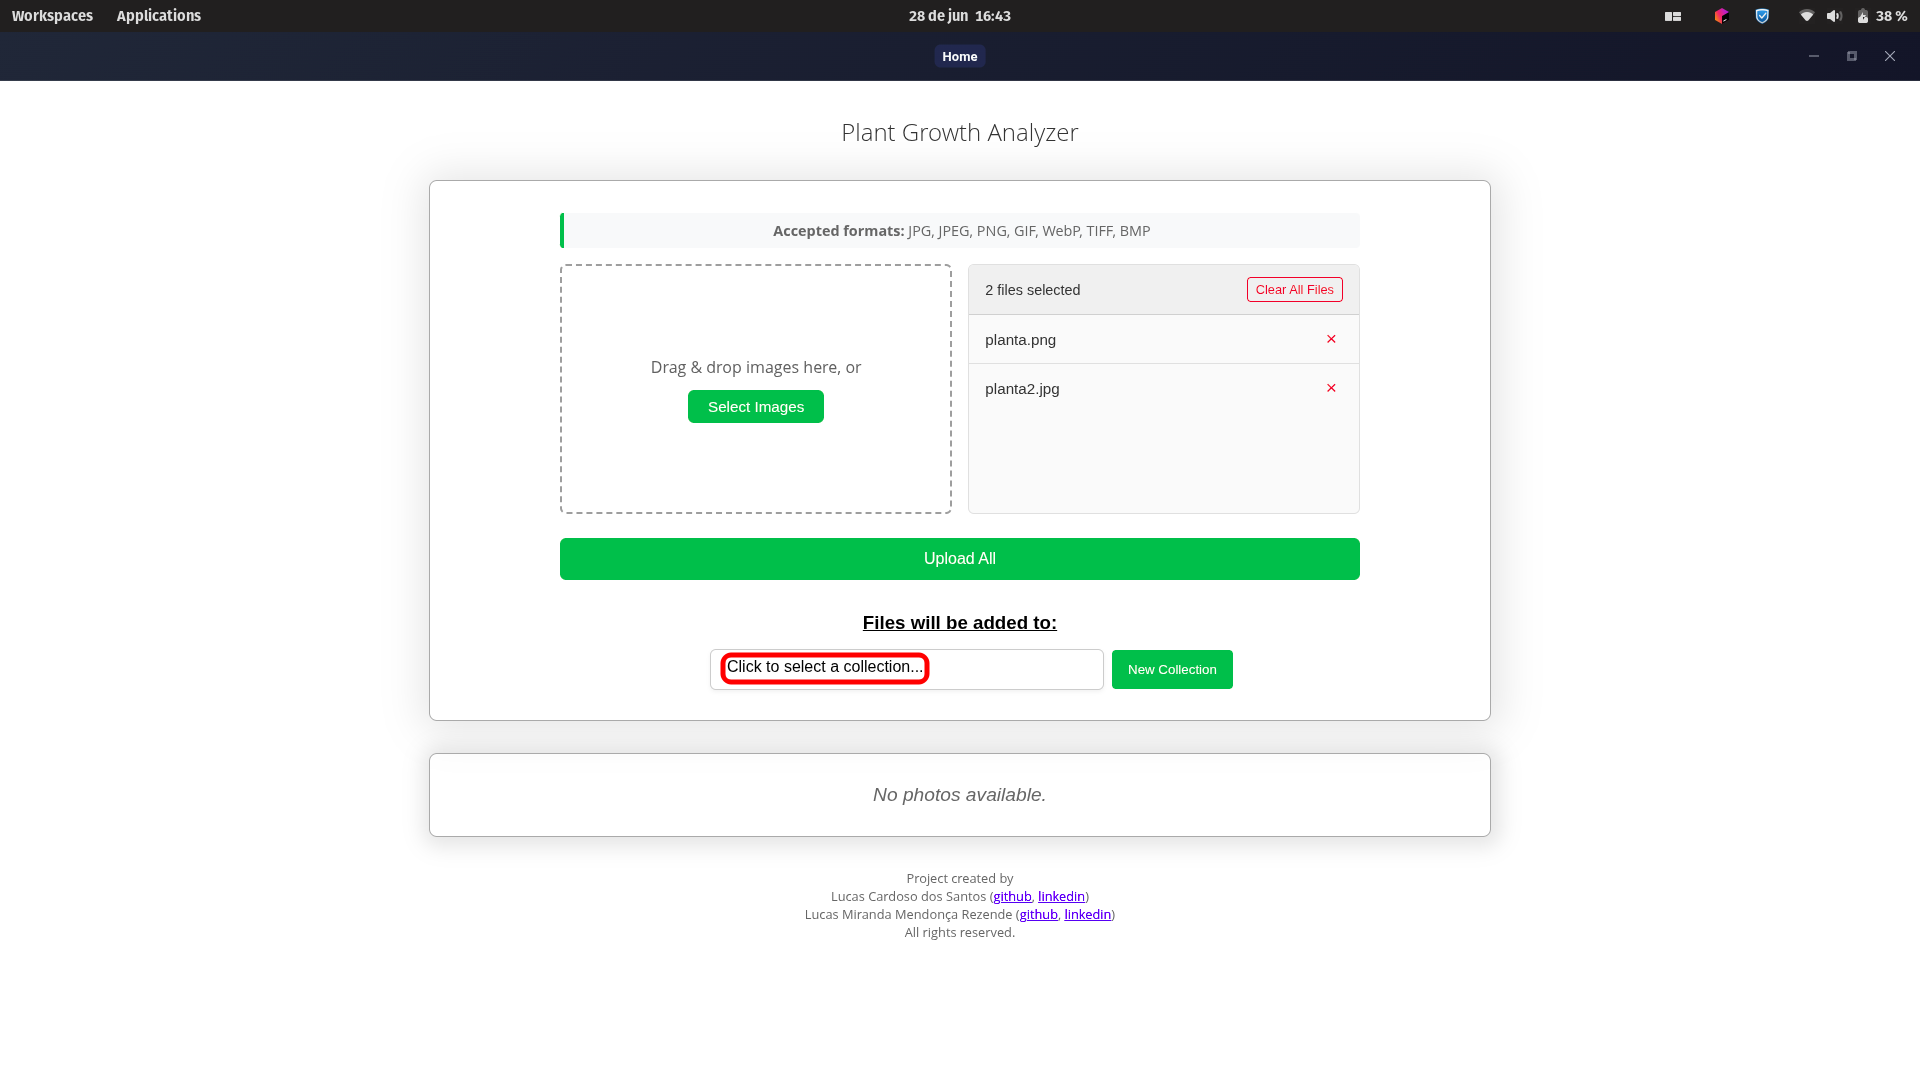
\includegraphics[width=1\textwidth]{../figures/screens/uc002/Screenshot from 2025-06-28 16-43-50.png}
    \caption{Adicionar imagens a uma coleção já criada. Fonte: os autores}
    \label{fig:uc002-screen5}
\end{figure}

\begin{figure}[H]
    \centering
    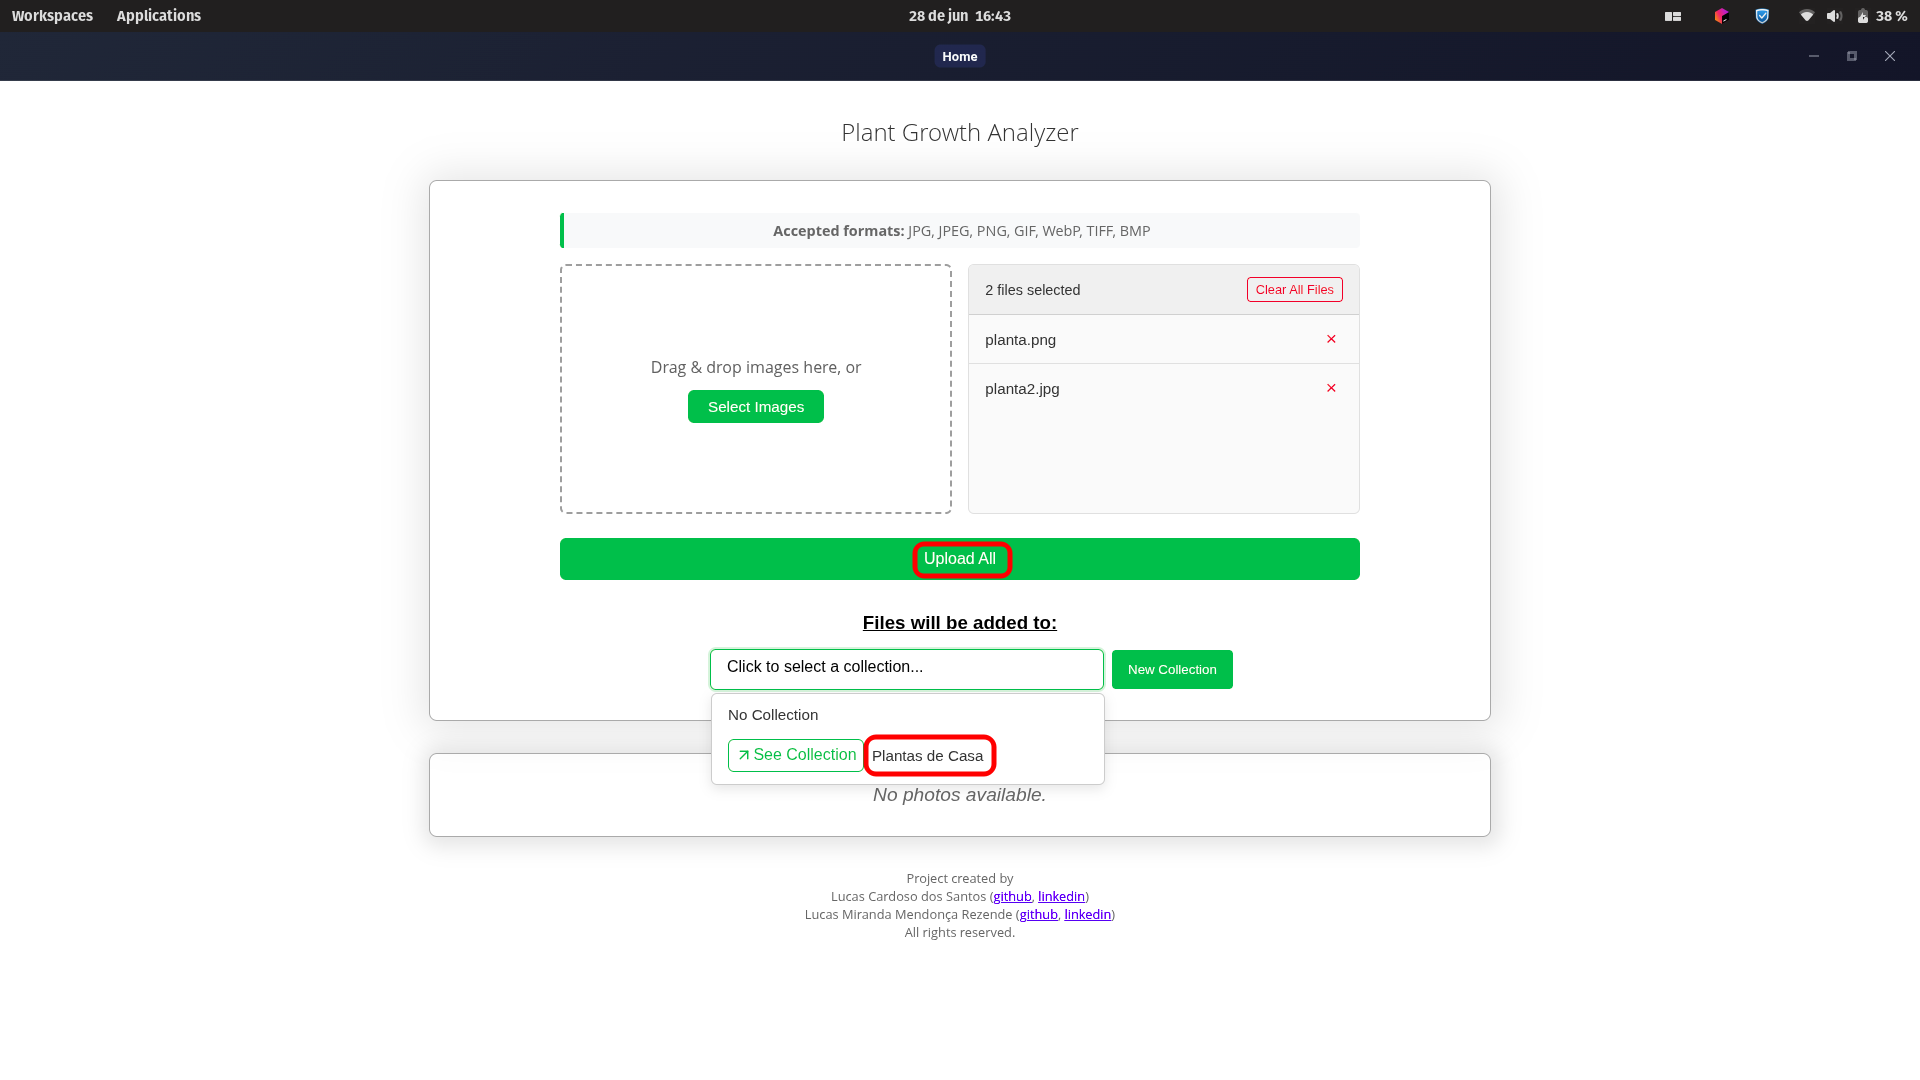
\includegraphics[width=1\textwidth]{../figures/screens/uc002/Screenshot from 2025-06-28 16-43-54.png}
    \caption{Coleção desejada selecionada. Fonte: os autores}
    \label{fig:uc002-screen6}
\end{figure}

\begin{figure}[H]
    \centering
    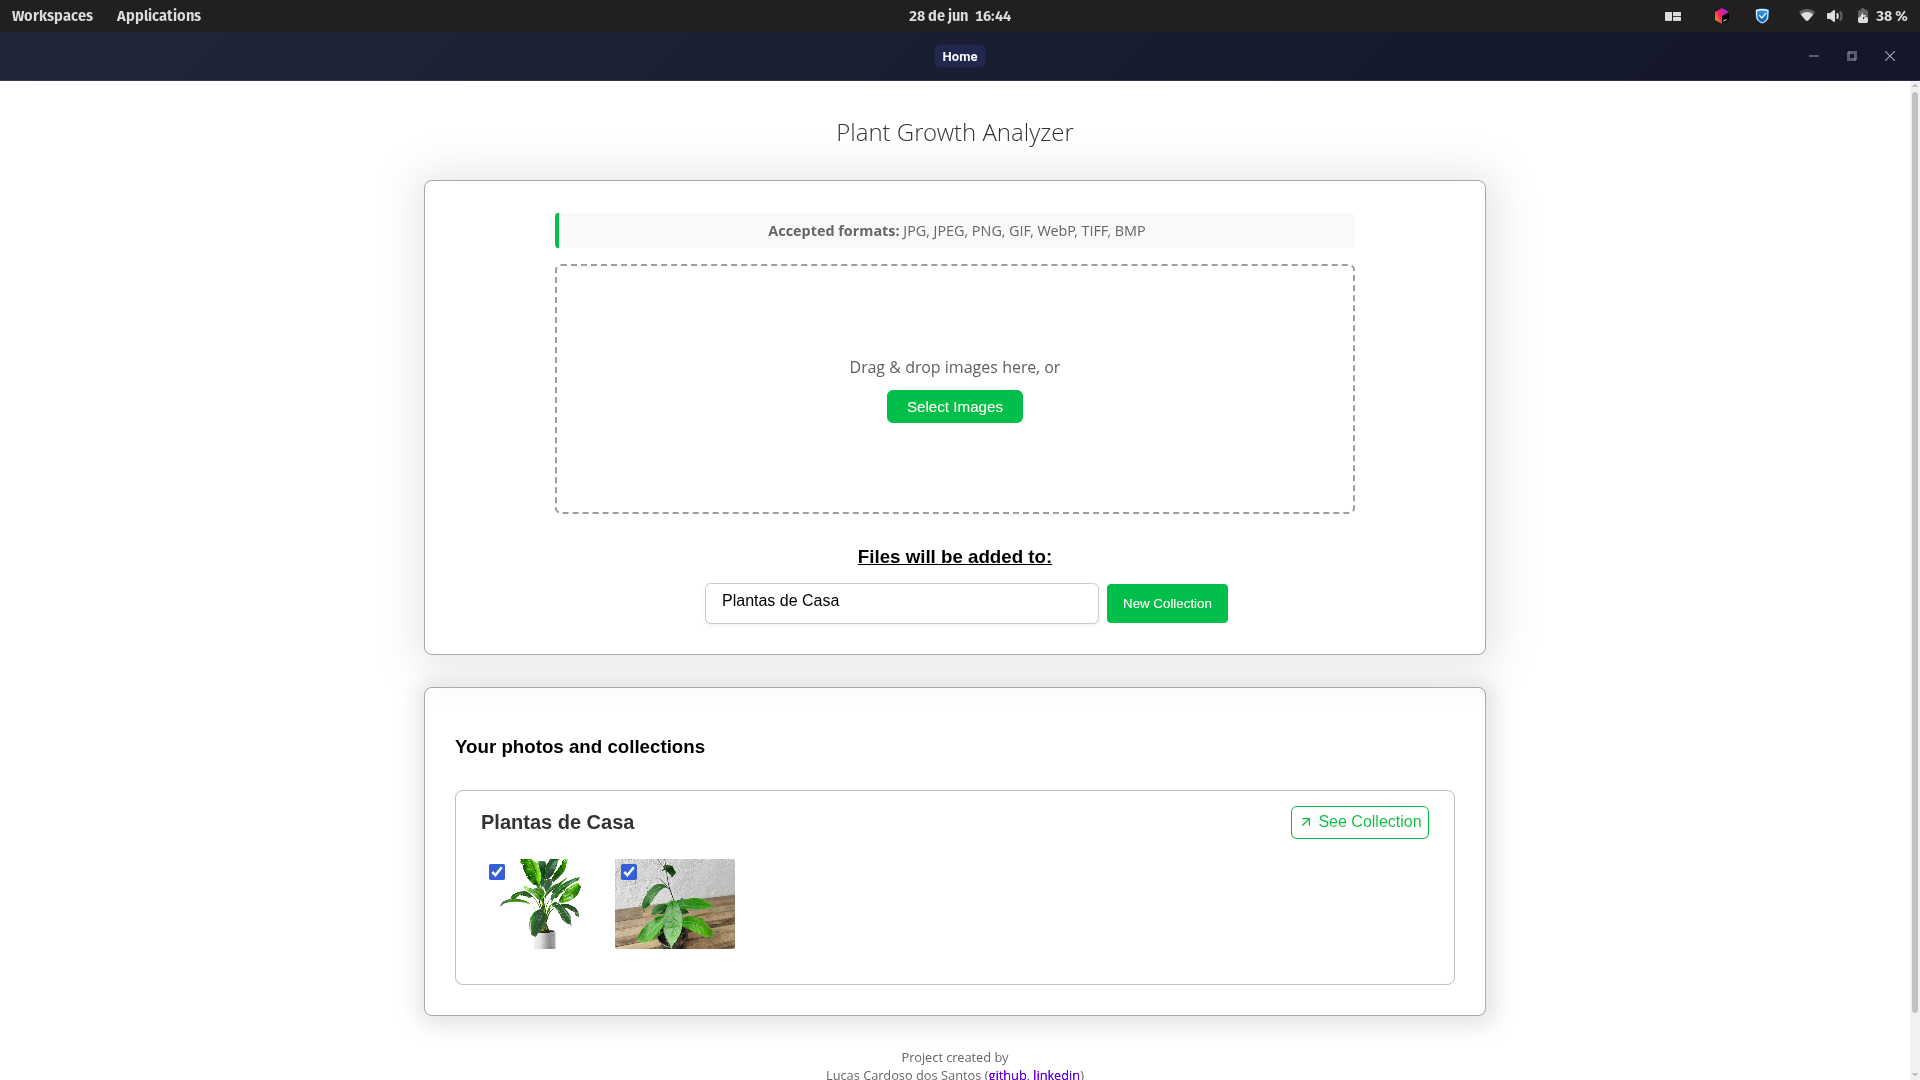
\includegraphics[width=1\textwidth]{../figures/screens/uc002/Screenshot from 2025-06-28 16-44-12.png}
    \caption{Múltiplas imagens adicionadas. Fonte: os autores}
    \label{fig:uc002-screen8}
\end{figure}

\section{Adicionar foto à coleção}

\subsection{HTA Model}

\begin{figure}[H]
    \centering
    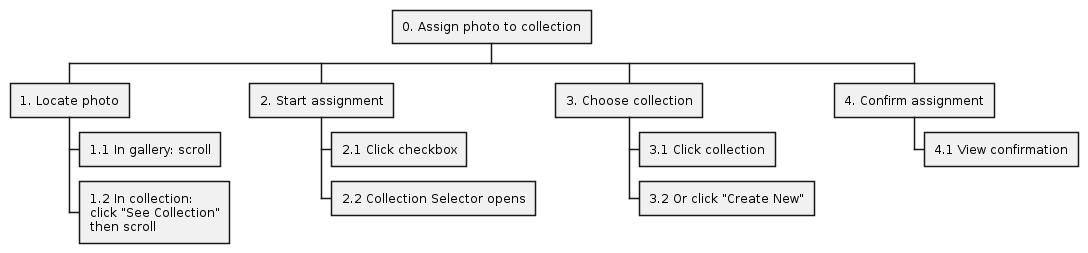
\includegraphics[width=0.9\textwidth]{../figures/hta/UC003.png}
    \caption{HTA Model para o caso de uso: Adicionar foto à coleção. Fonte: os autores}
    \label{fig:hta-uc003}
\end{figure}

\subsection{Diagrama de Sequência}

\begin{figure}[H]
    \centering
    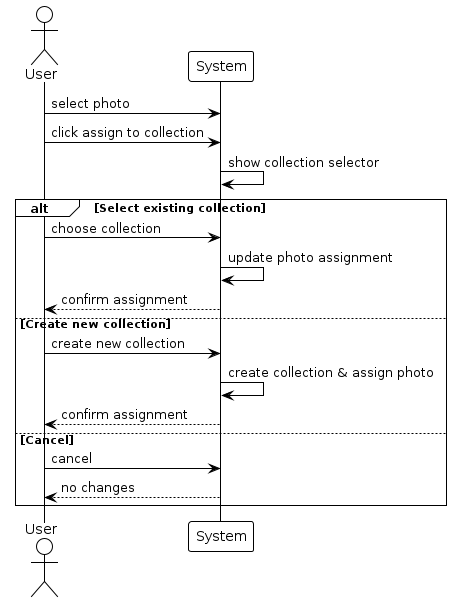
\includegraphics[width=0.9\textwidth]{../figures/dss/UC003.png}
    \caption{Diagrama de sequência para o caso de uso: Adicionar foto à coleção. Fonte: os autores}
    \label{fig:dss-uc003}
\end{figure}

\subsection{Telas da Aplicação}

\begin{figure}[H]
    \centering
    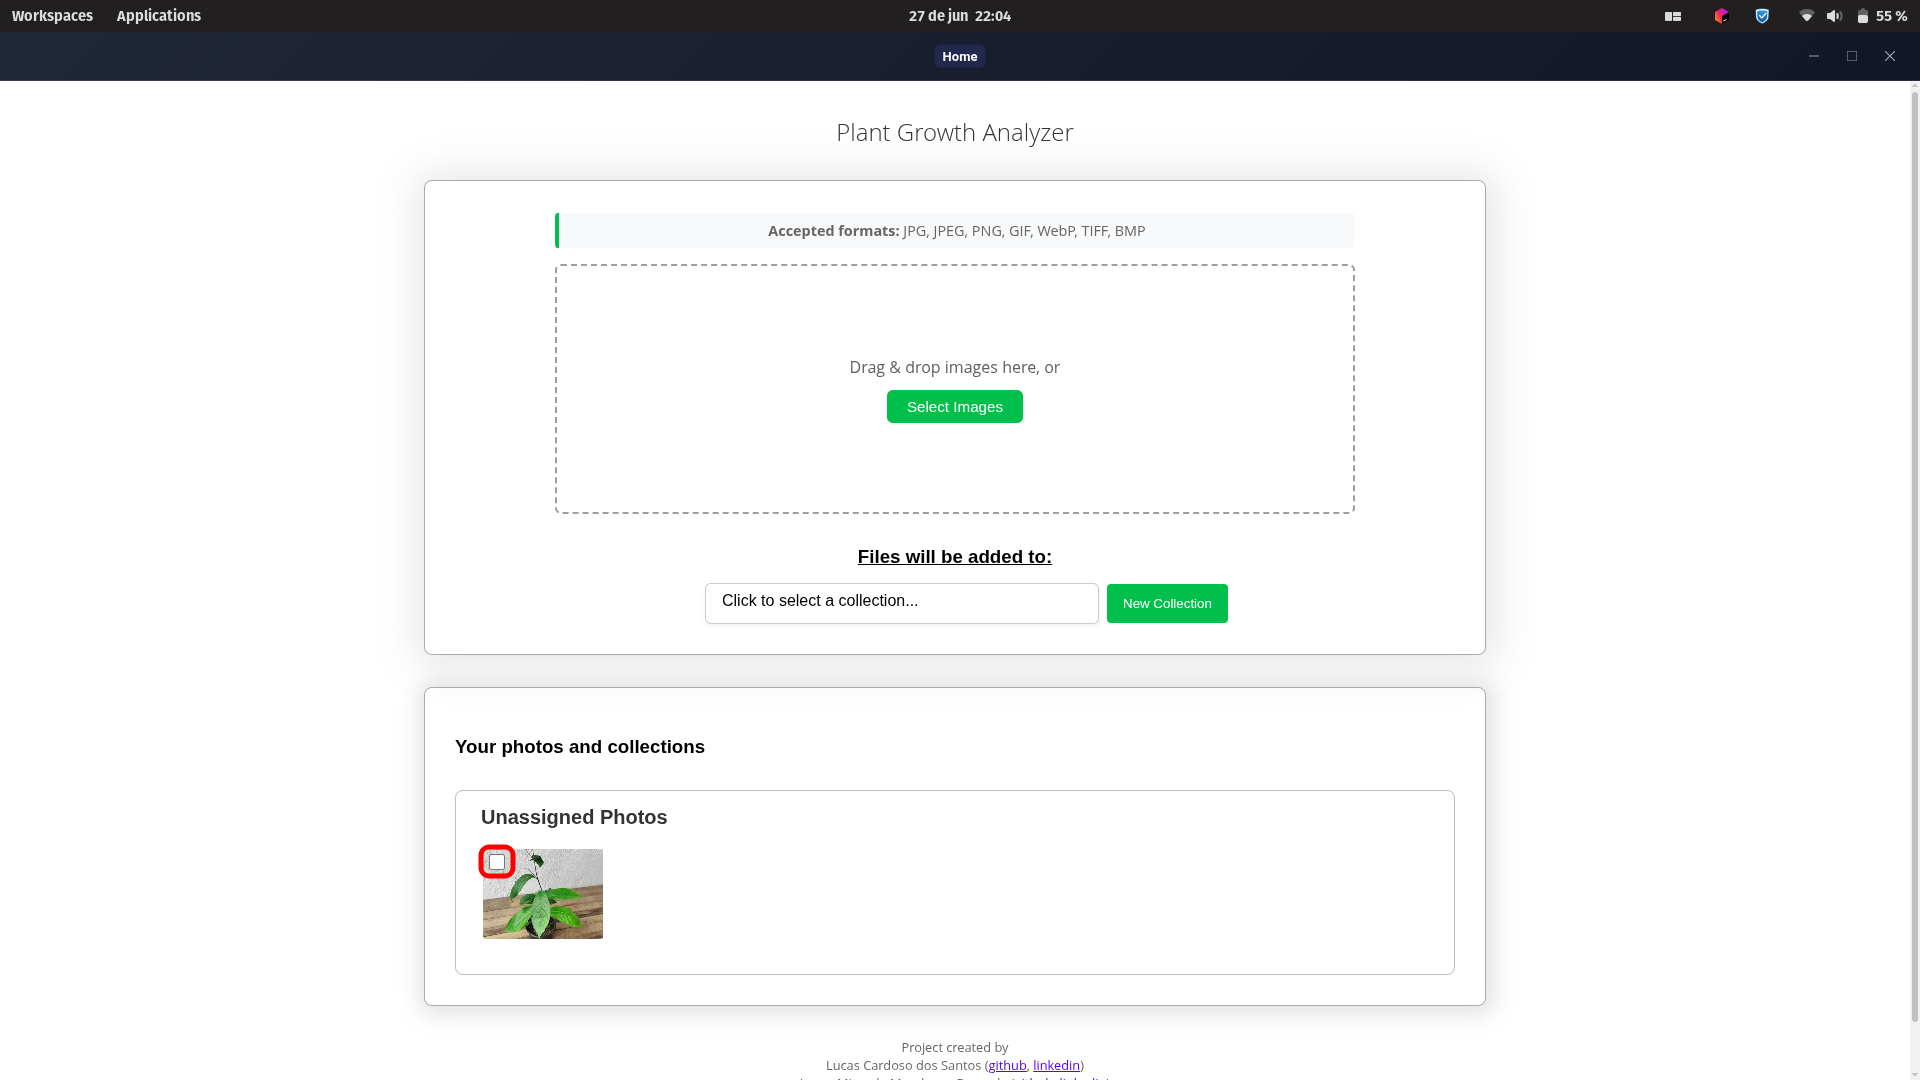
\includegraphics[width=1\textwidth]{../figures/screens/uc003/Screenshot from 2025-06-27 22-04-12.png}
    \caption{Selecionar foto sem coleção. Fonte: os autores}
    \label{fig:uc003-screen1}
\end{figure}

\begin{figure}[H]
    \centering
    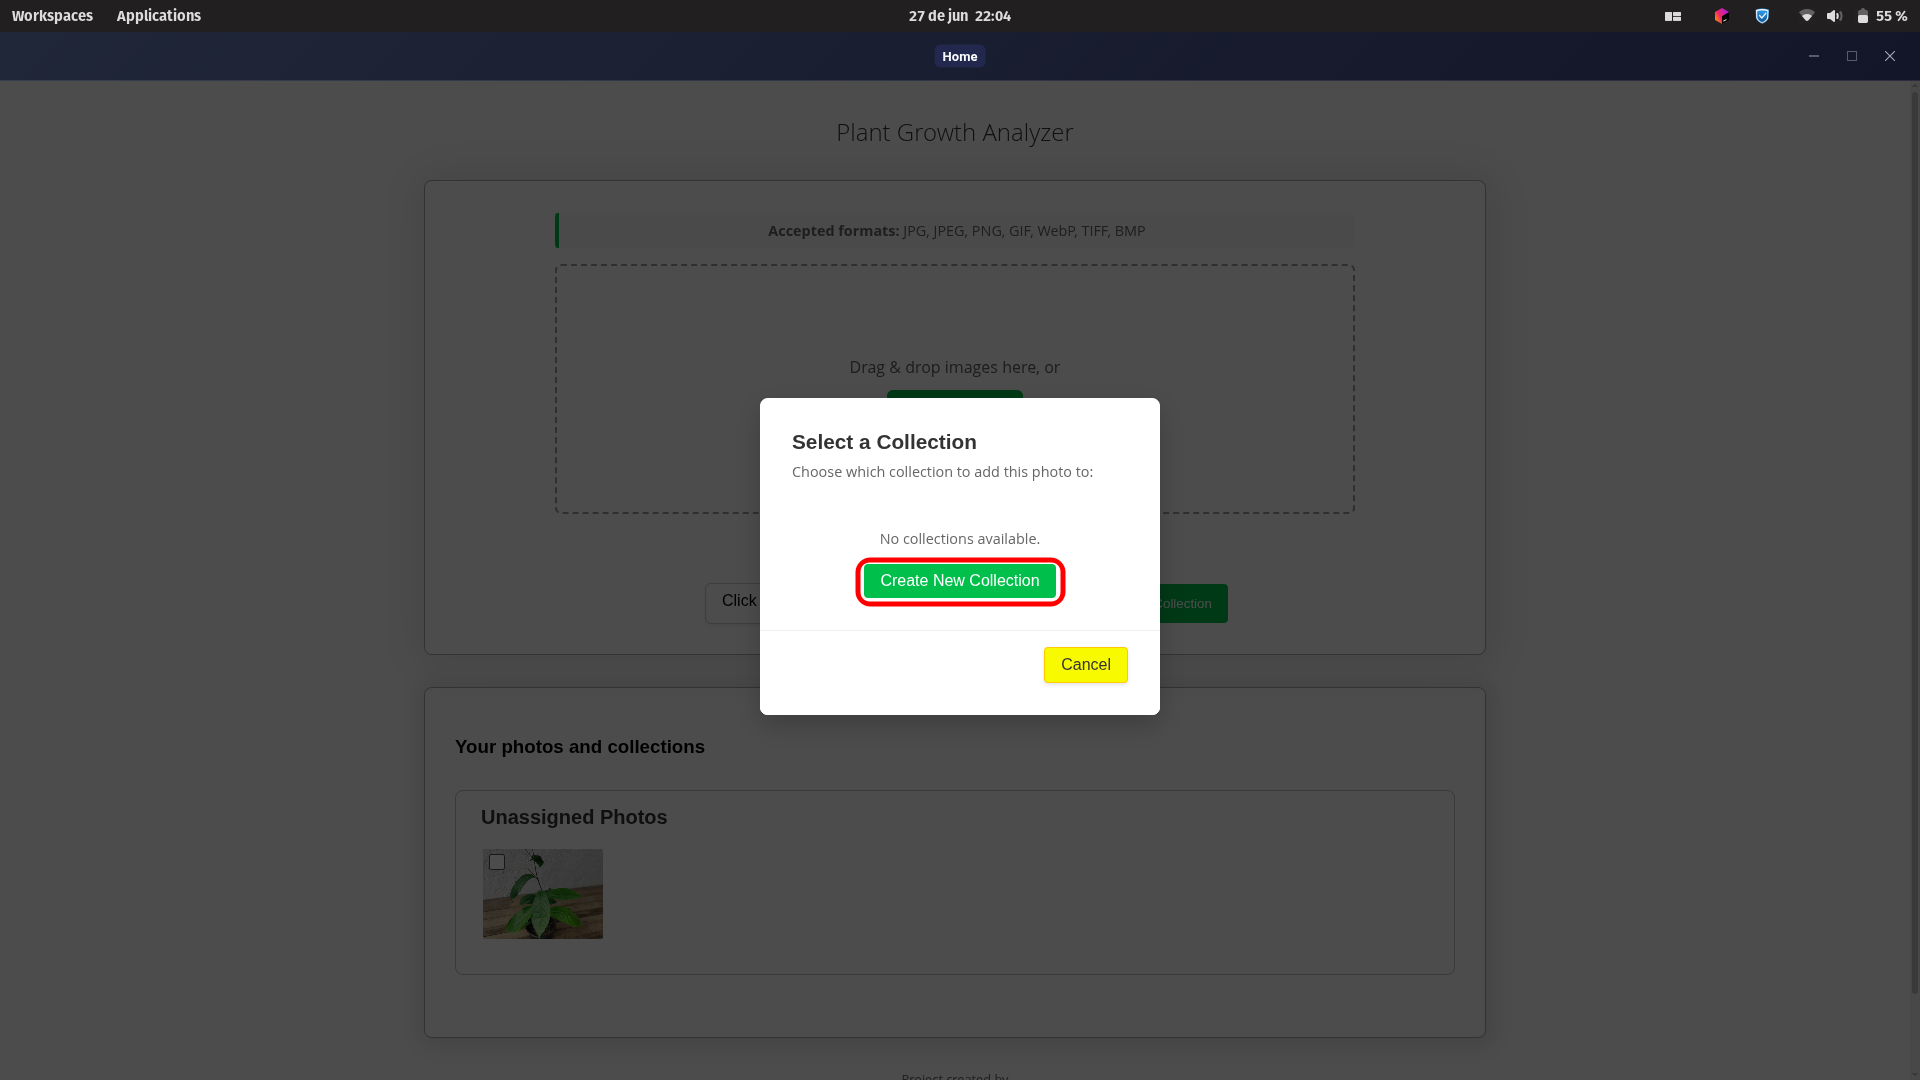
\includegraphics[width=1\textwidth]{../figures/screens/uc003/Screenshot from 2025-06-27 22-04-19.png}
    \caption{Não há coleções já ciradas: criar uma nova. Fonte: os autores}
    \label{fig:uc003-screen2}
\end{figure}

\begin{figure}[H]
    \centering
    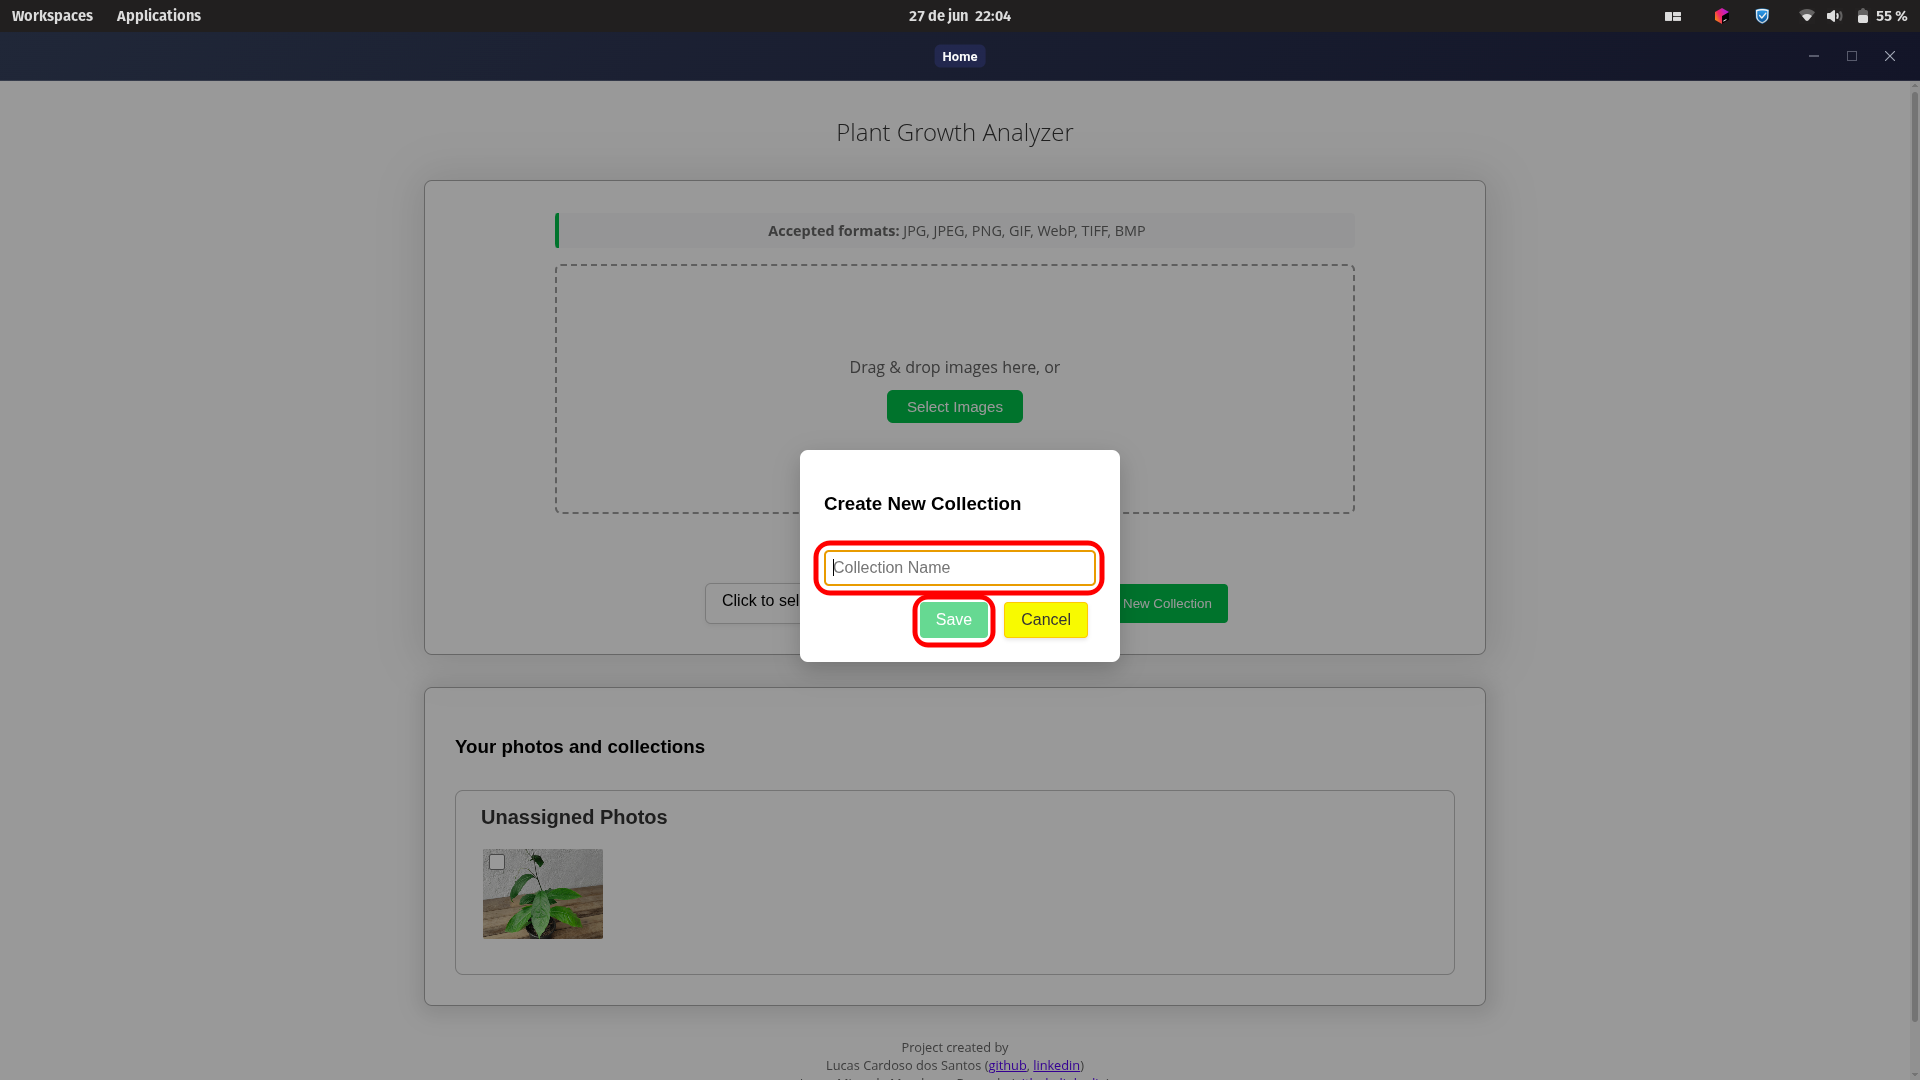
\includegraphics[width=1\textwidth]{../figures/screens/uc003/Screenshot from 2025-06-27 22-04-26.png}
    \caption{Inserir nome da coleção. Fonte: os autores}
    \label{fig:uc003-screen3}
\end{figure}

\begin{figure}[H]
    \centering
    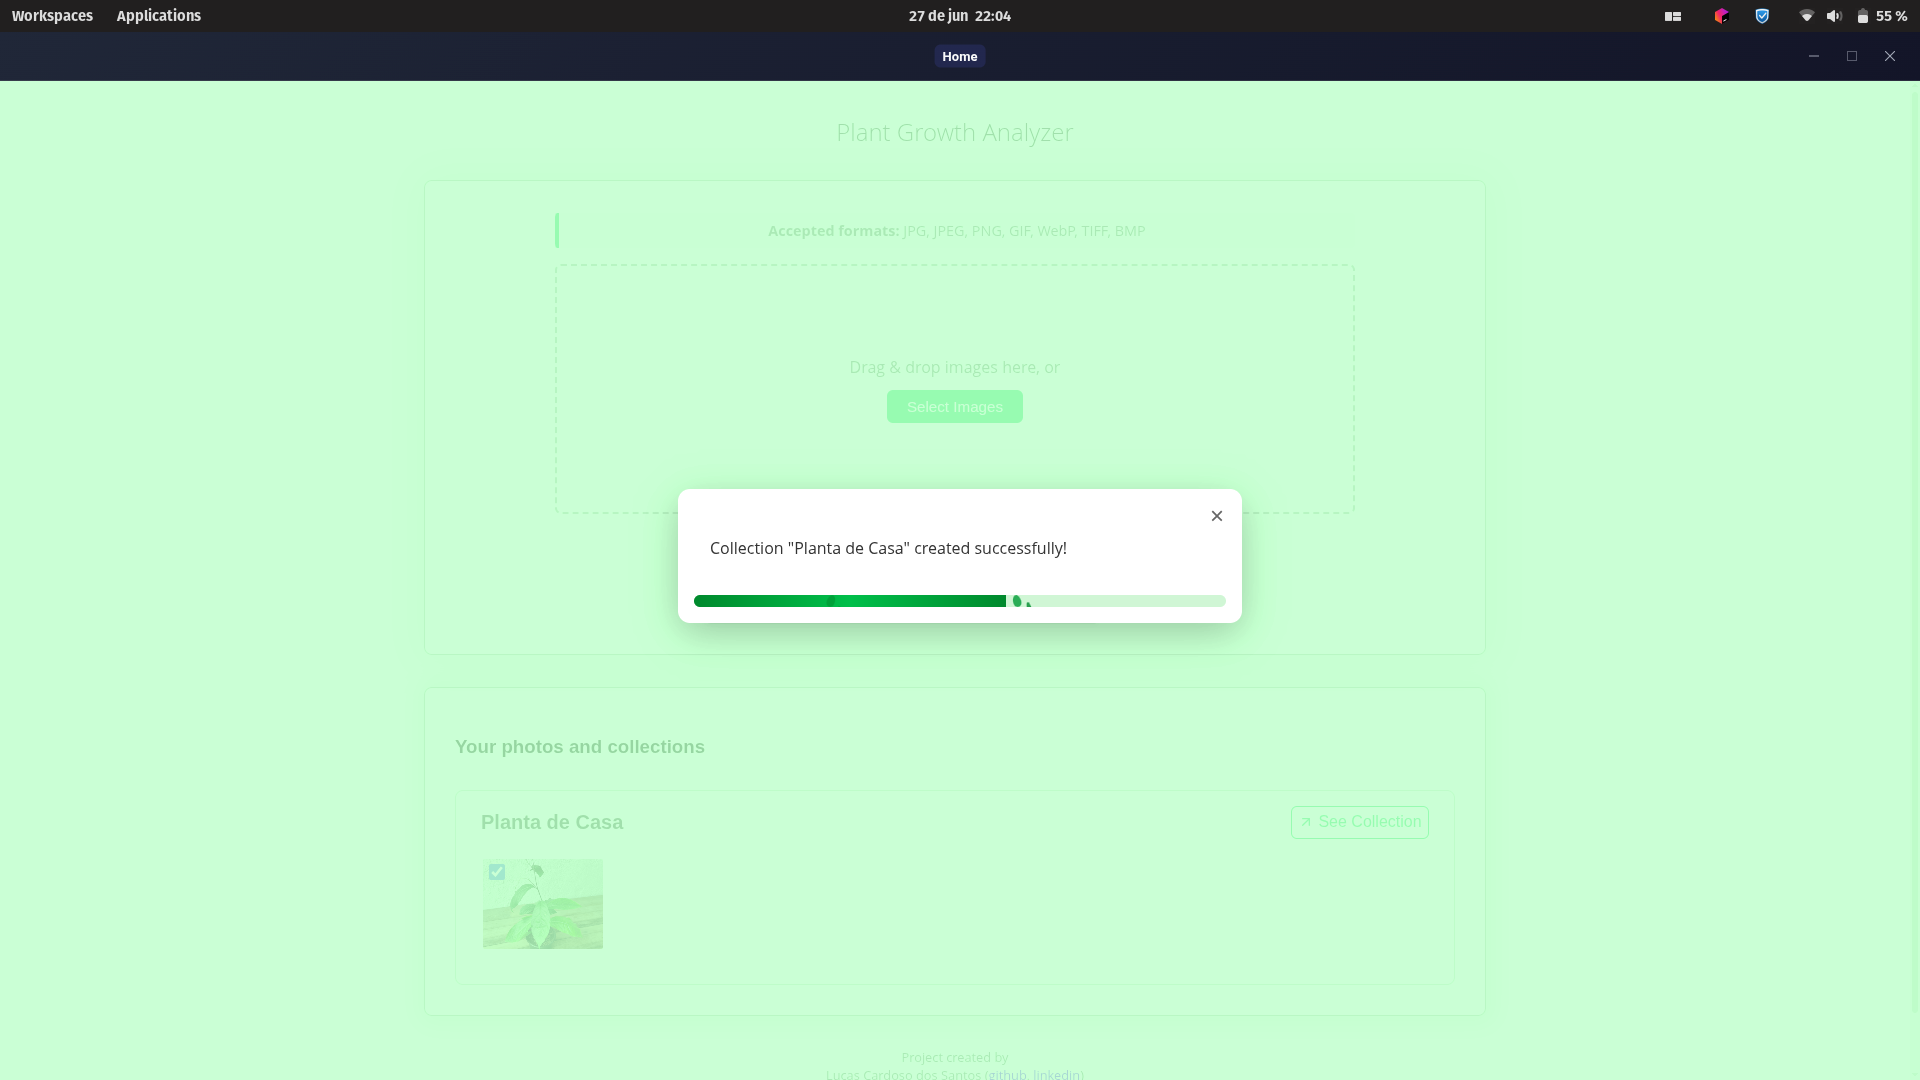
\includegraphics[width=1\textwidth]{../figures/screens/uc003/Screenshot from 2025-06-27 22-04-40.png}
    \caption{Coleção criada com sucesso. Fonte: os autores}
    \label{fig:uc003-screen4}
\end{figure}

\begin{figure}[H]
    \centering
    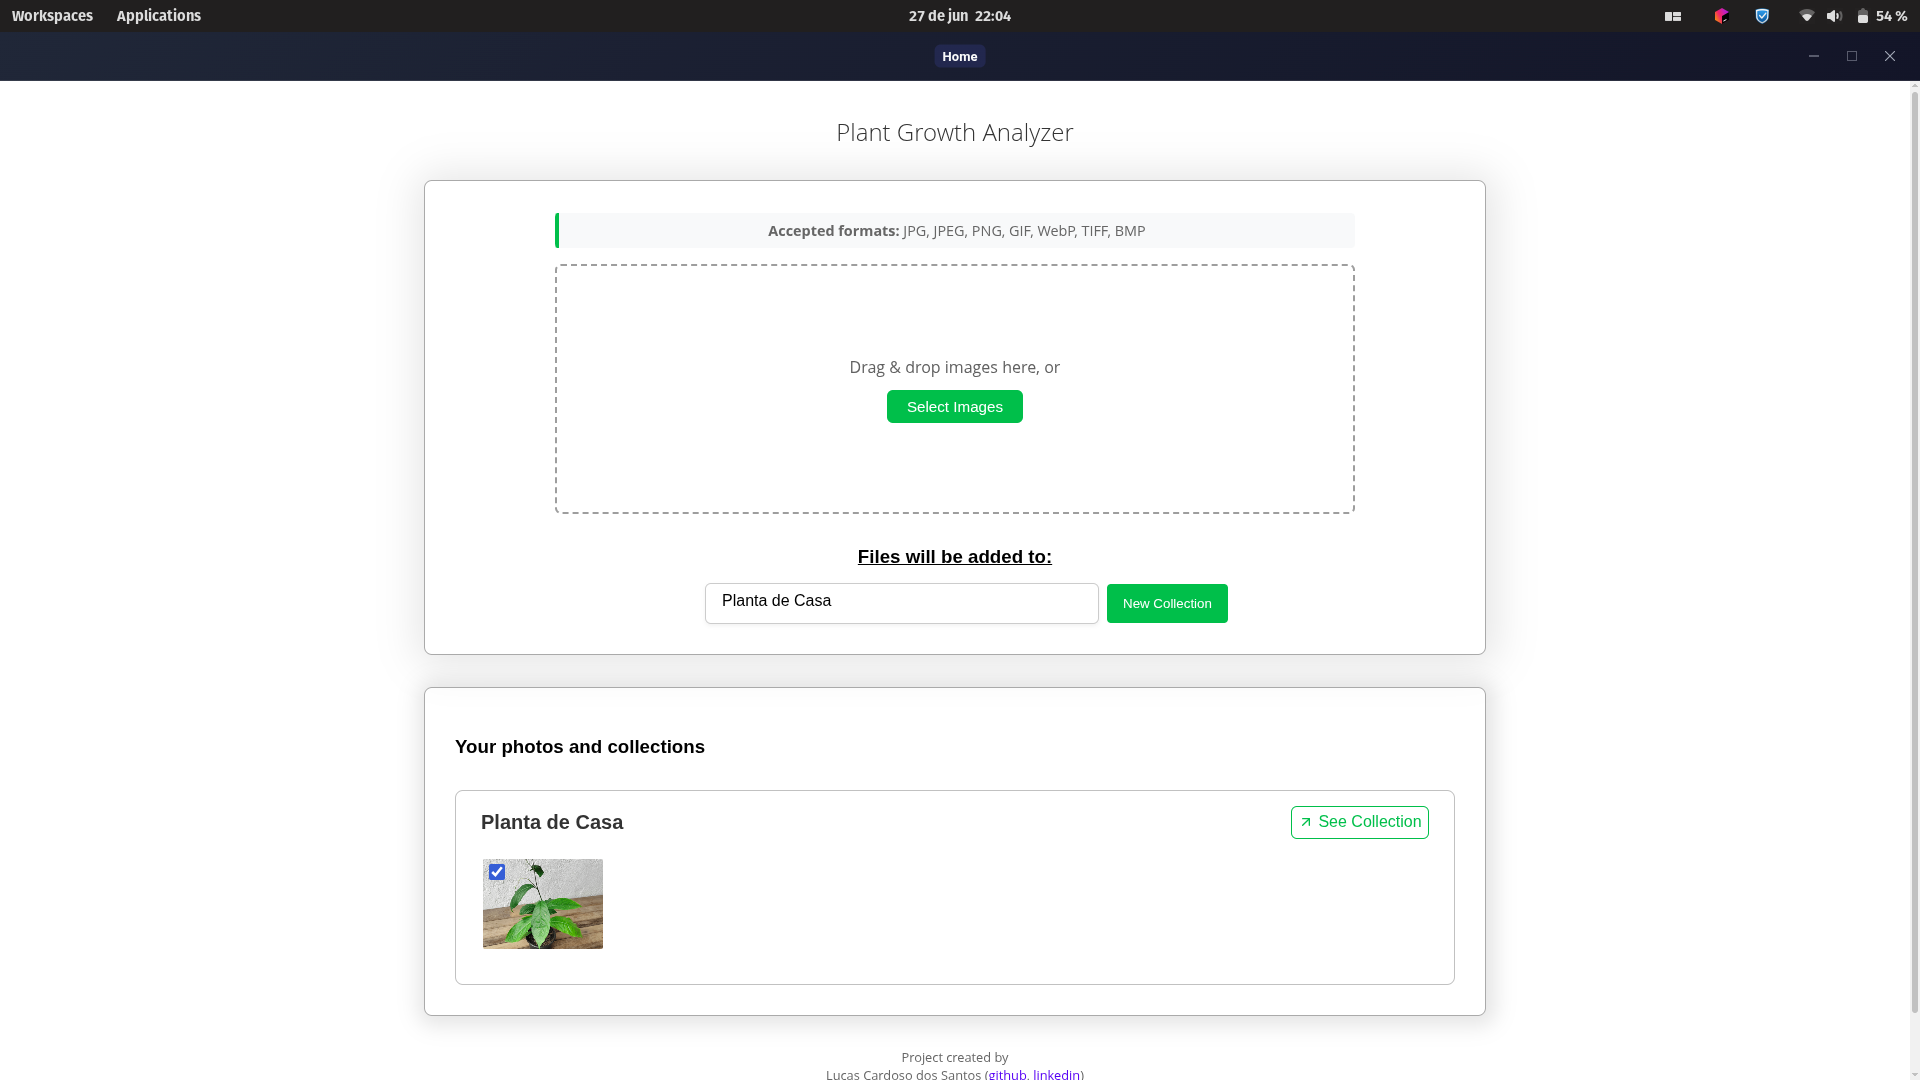
\includegraphics[width=1\textwidth]{../figures/screens/uc003/Screenshot from 2025-06-27 22-04-48.png}
    \caption{Foto adicionada com sucesso. Fonte: os autores}
    \label{fig:uc003-screen5}
\end{figure}

\section{Remover foto de coleção}

\subsection{HTA Model}

\begin{figure}[H]
    \centering
    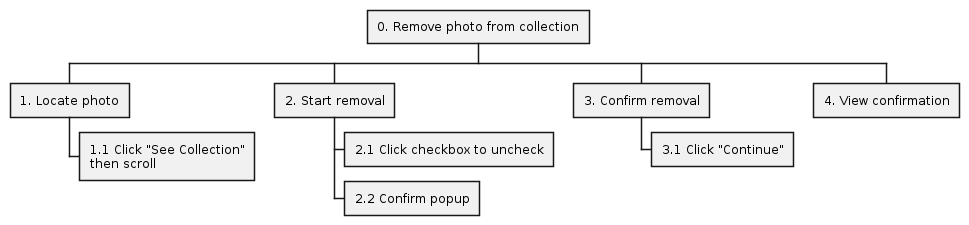
\includegraphics[width=0.9\textwidth]{../figures/hta/UC004.png}
    \caption{HTA Model para o caso de uso: Remover foto de coleção. Fonte: os autores}
    \label{fig:hta-uc004}
\end{figure}

\subsection{Diagrama de Sequência}

\begin{figure}[H]
    \centering
    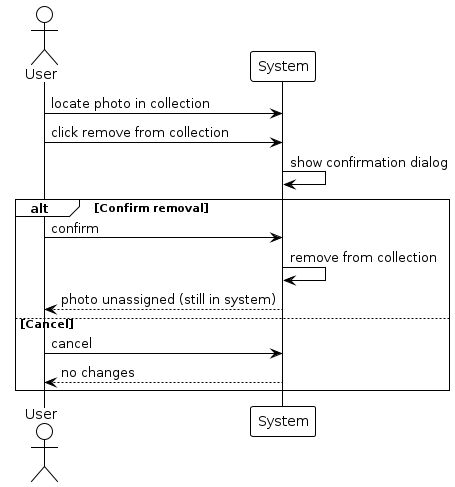
\includegraphics[width=0.9\textwidth]{../figures/dss/UC004.png}
    \caption{Diagrama de sequência para o caso de uso: Remover foto de coleção. Fonte: os autores}
    \label{fig:dss-uc004}
\end{figure}

\subsection{Telas da Aplicação}

\begin{figure}[H]
    \centering
    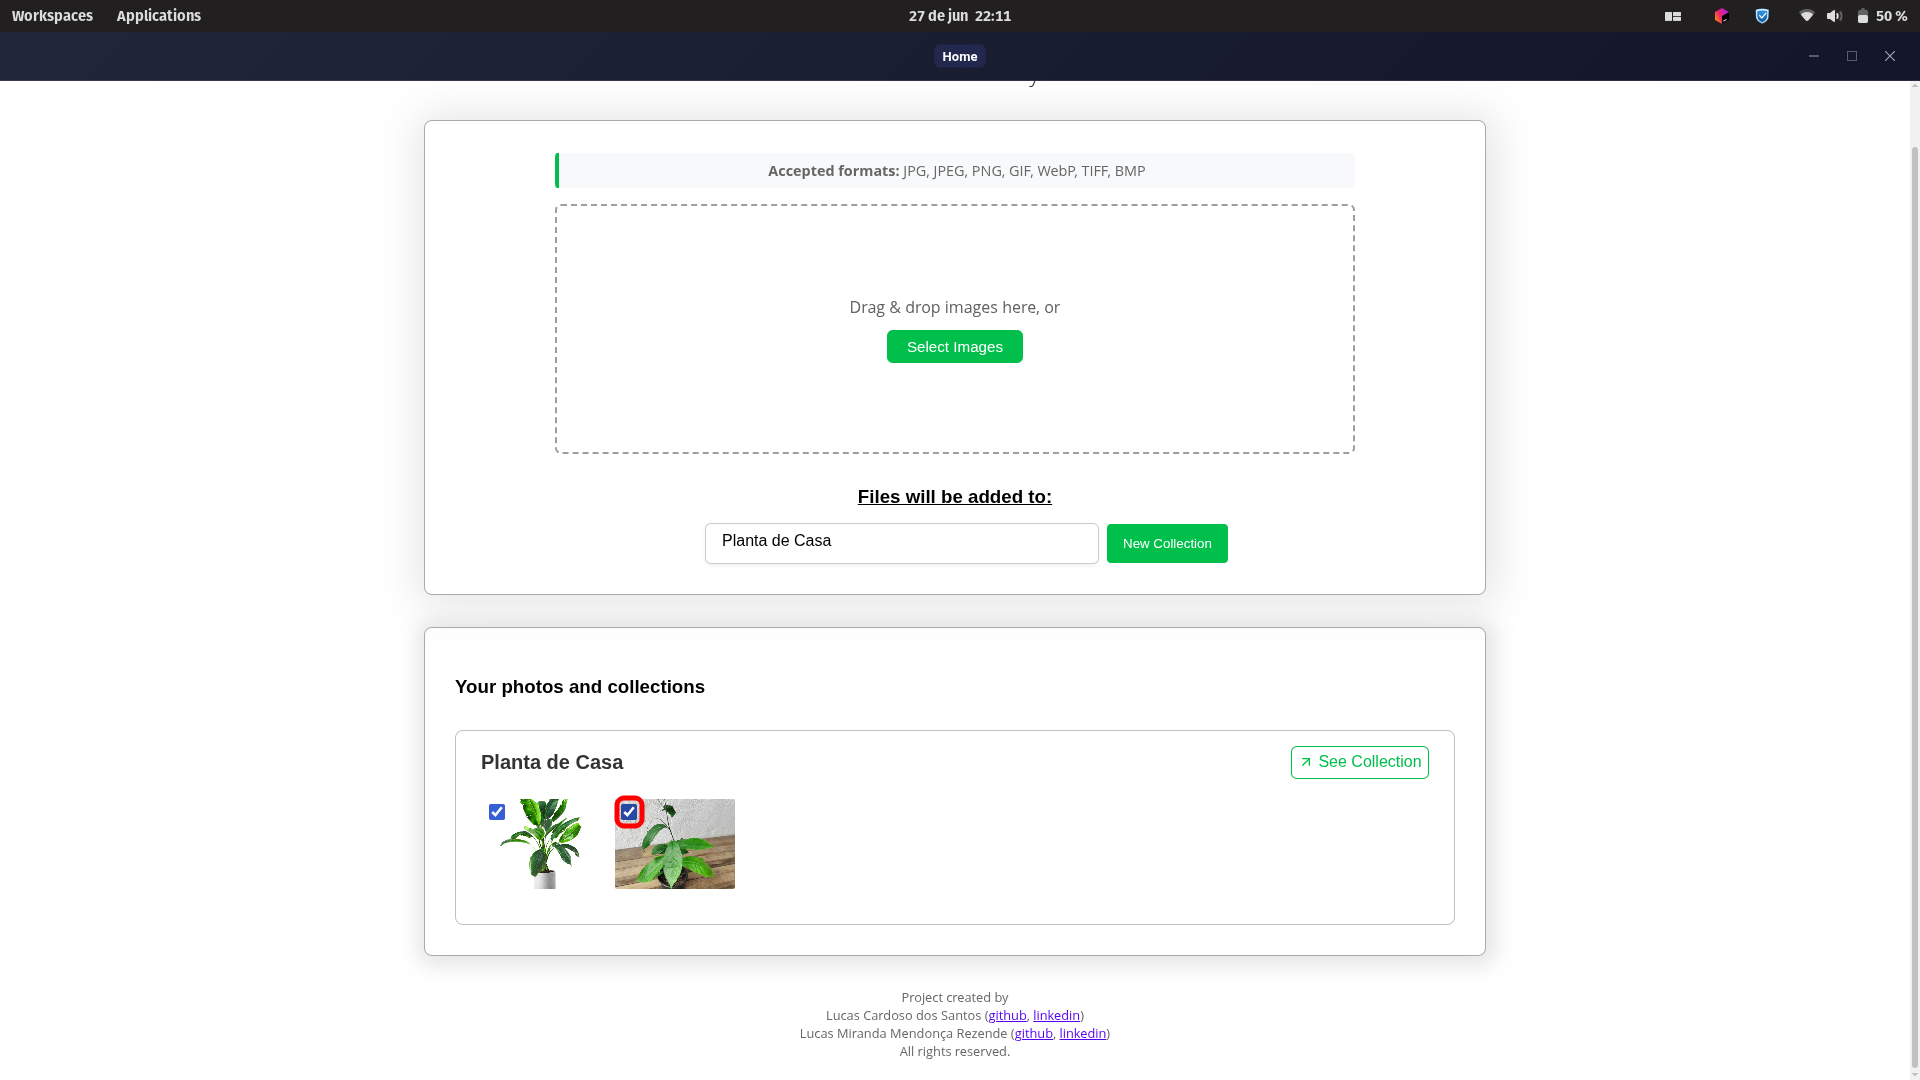
\includegraphics[width=1\textwidth]{../figures/screens/uc004/Screenshot from 2025-06-27 22-11-19.png}
    \caption{Selecionar imagem que se deseja remover da coleção. Fonte: os autores}
    \label{fig:uc004-screen1}
\end{figure}

\begin{figure}[H]
    \centering
    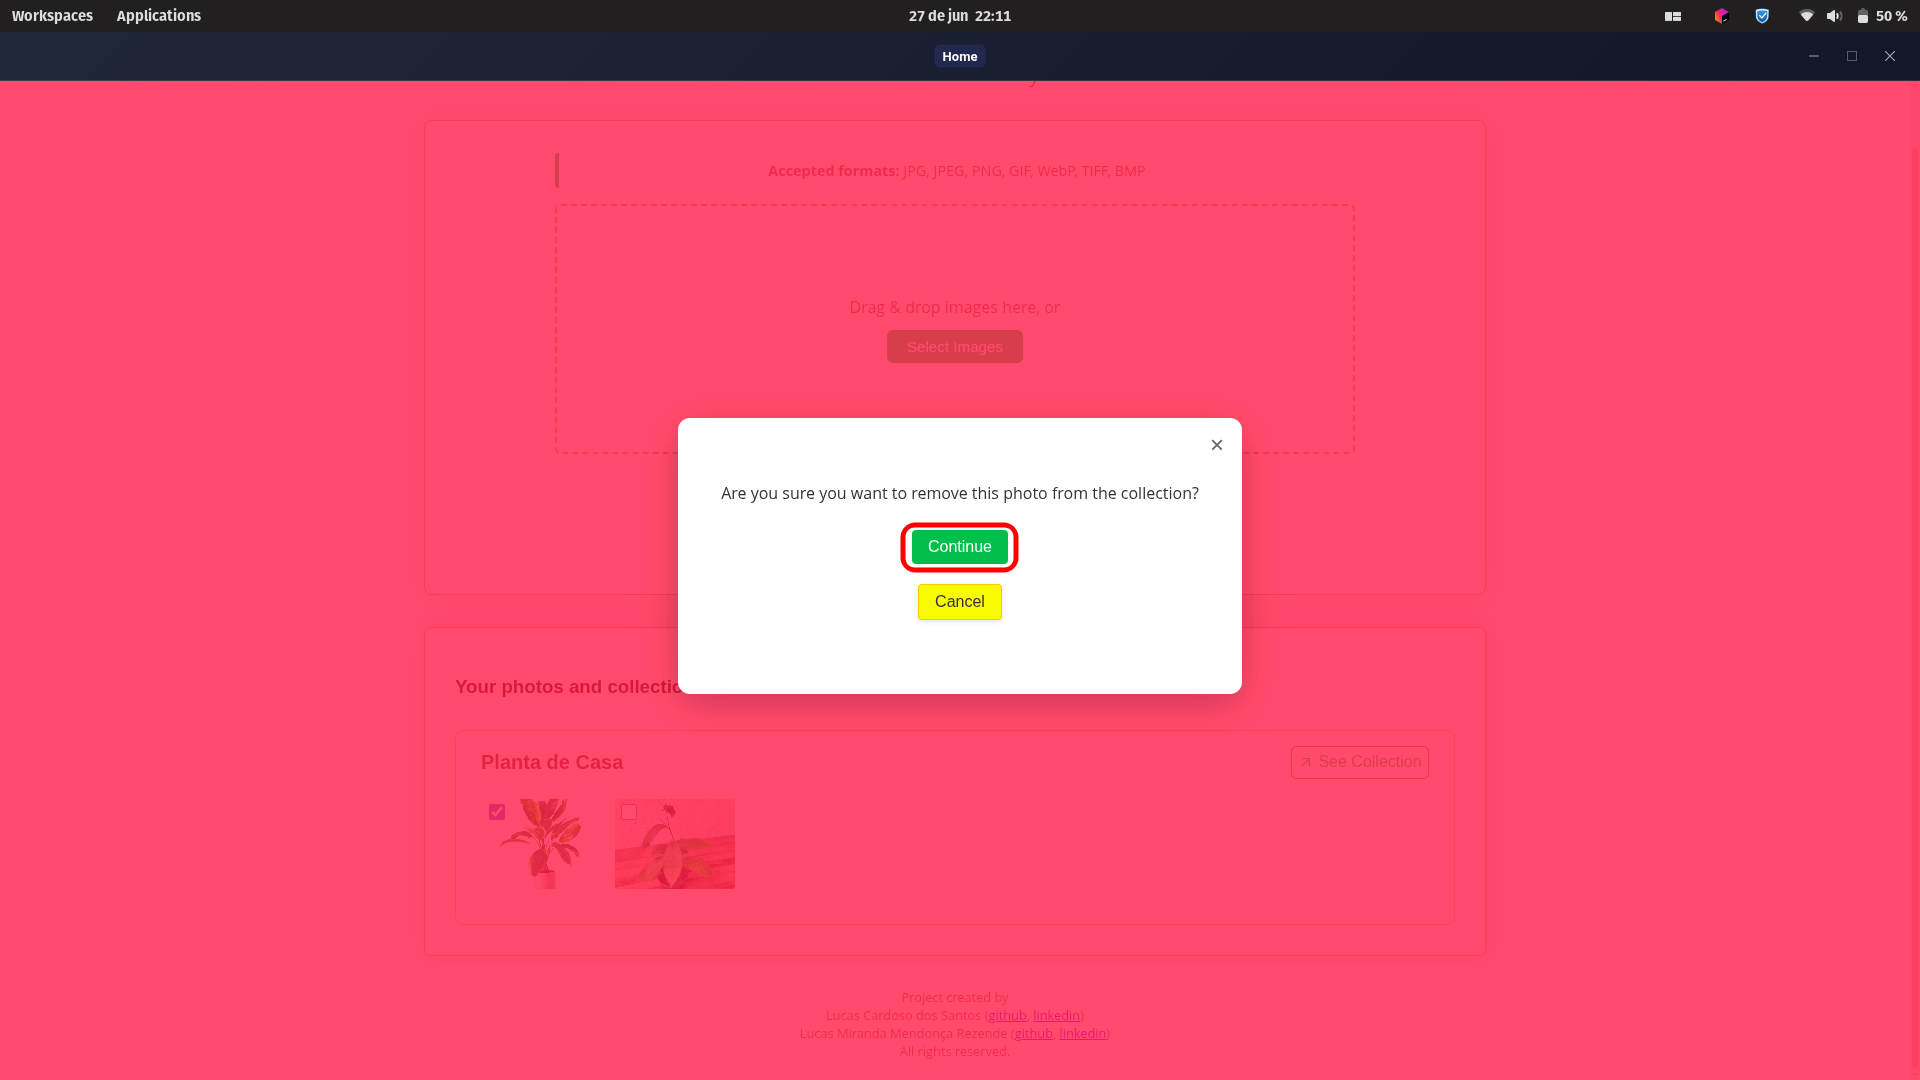
\includegraphics[width=1\textwidth]{../figures/screens/uc004/Screenshot from 2025-06-27 22-11-24.png}
    \caption{Confirmar ação. Fonte: os autores}
    \label{fig:uc004-screen2}
\end{figure}

\begin{figure}[H]
    \centering
    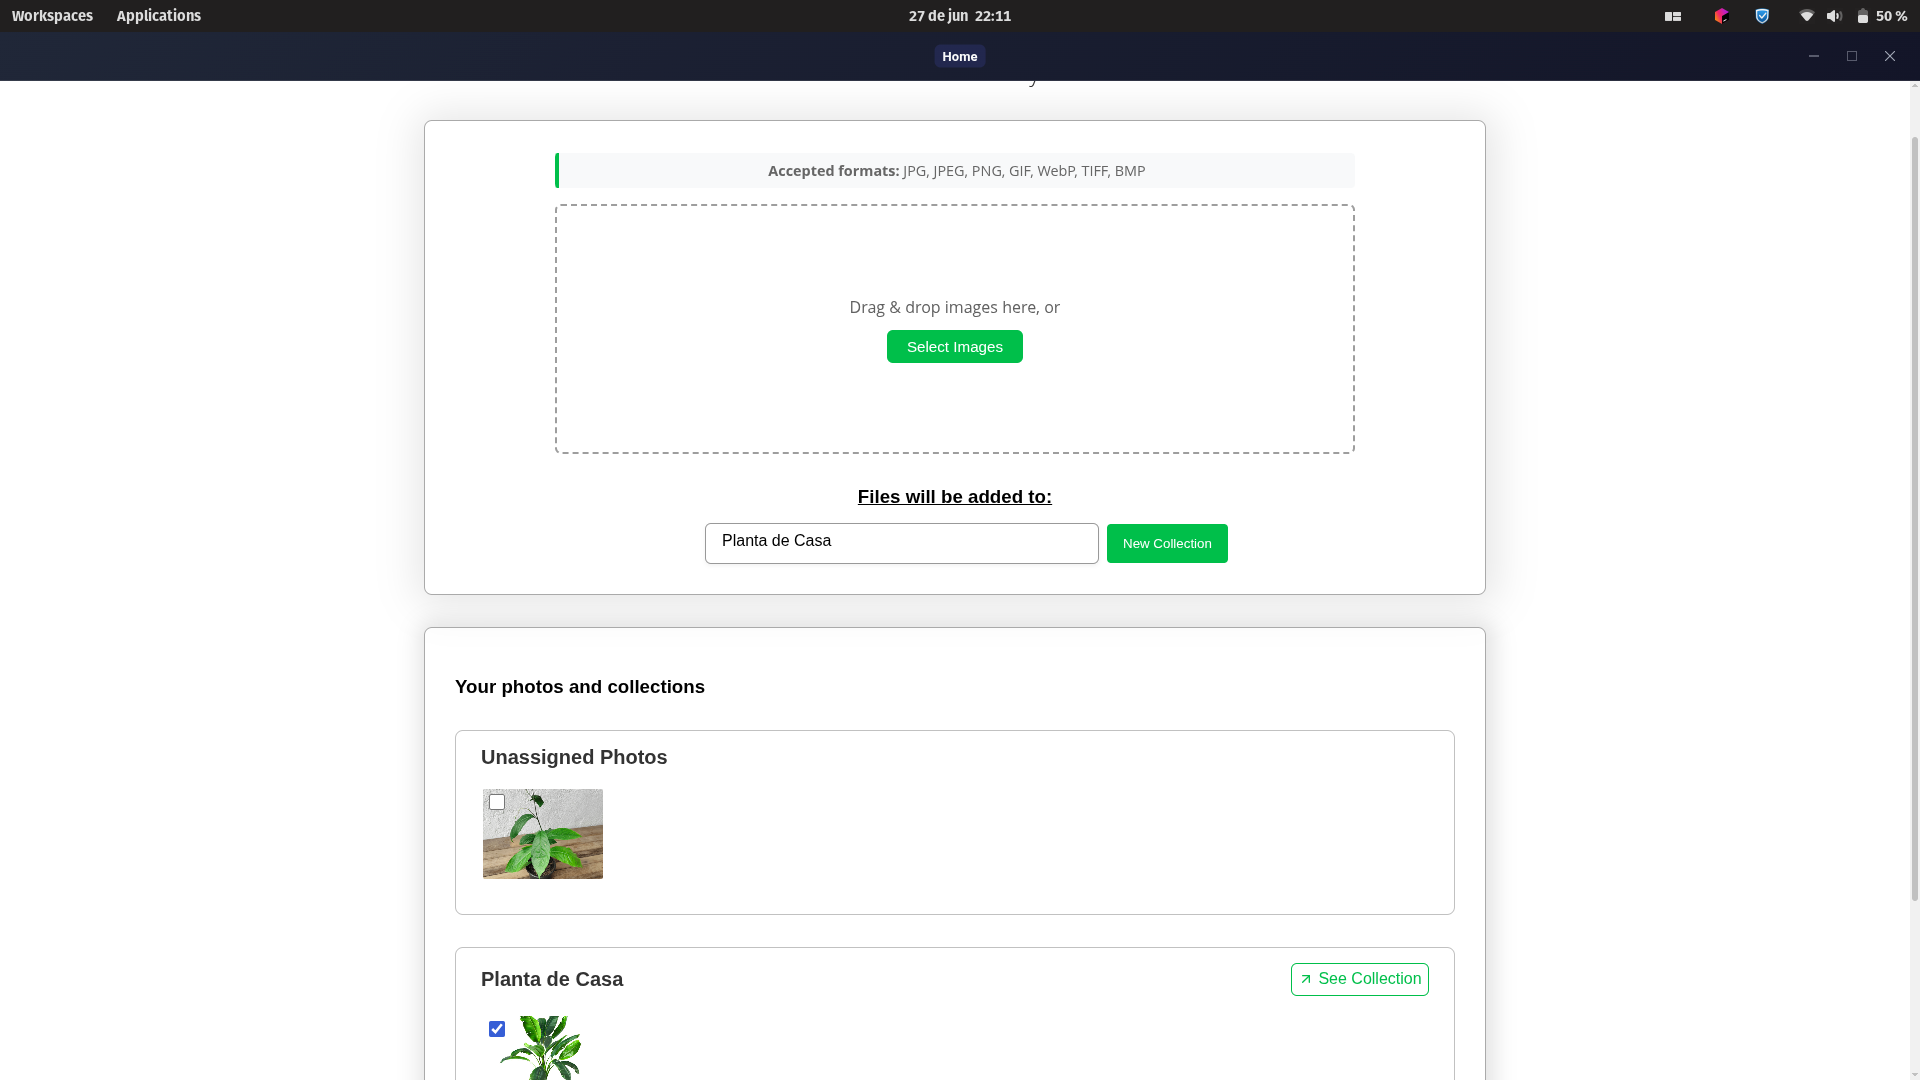
\includegraphics[width=1\textwidth]{../figures/screens/uc004/Screenshot from 2025-06-27 22-11-28.png}
    \caption{Foto removida com sucesso. Fonte: os autores}
    \label{fig:uc004-screen3}
\end{figure}

\section{Deletar foto}

\subsection{HTA Model}

\begin{figure}[H]
    \centering
    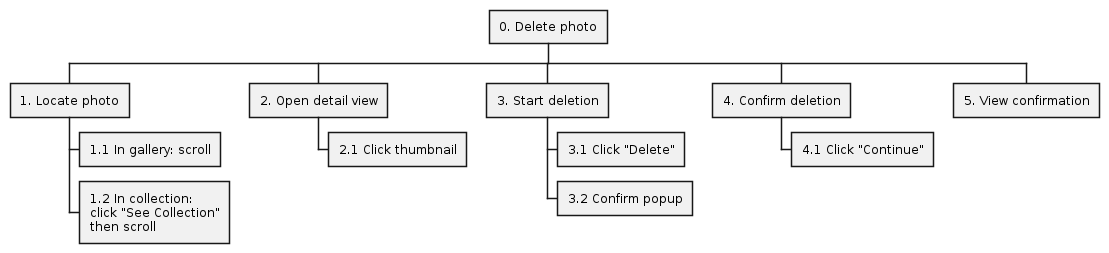
\includegraphics[width=0.9\textwidth]{../figures/hta/UC005.png}
    \caption{HTA Model para o caso de uso: Deletar foto. Fonte: os autores}
    \label{fig:hta-uc005}
\end{figure}

\subsection{Diagrama de Sequência}

\begin{figure}[H]
    \centering
    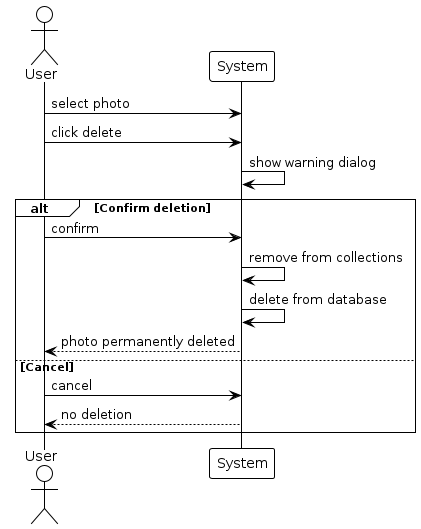
\includegraphics[width=0.9\textwidth]{../figures/dss/UC005.png}
    \caption{Diagrama de sequência para o caso de uso: Deletar foto. Fonte: os autores}
    \label{fig:dss-uc005}
\end{figure}

\subsection{Telas da Aplicação}

\begin{figure}[H]
    \centering
    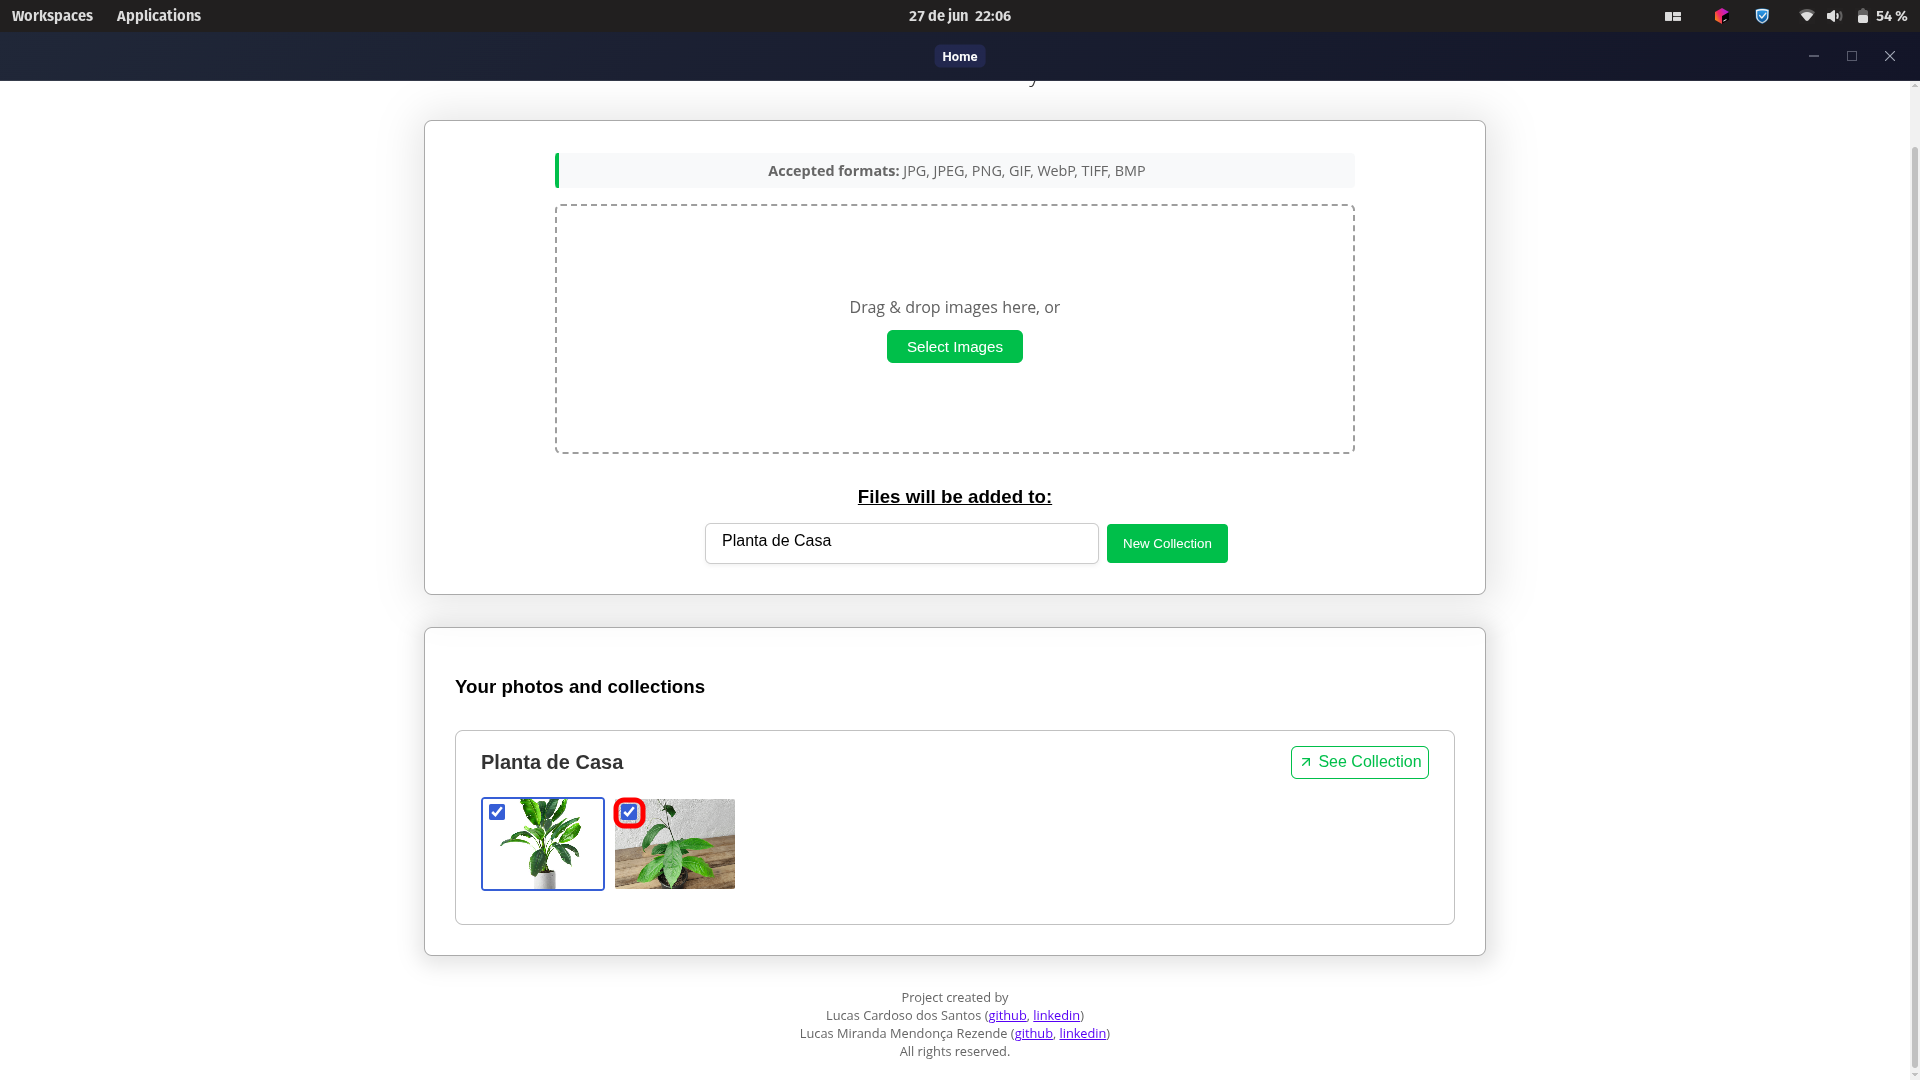
\includegraphics[width=1\textwidth]{../figures/screens/uc005/Screenshot from 2025-06-27 22-06-27.png}
    \caption{Selecionar foto que será excluída. Fonte: os autores}
    \label{fig:uc005-screen1}
\end{figure}

\begin{figure}[H]
    \centering
    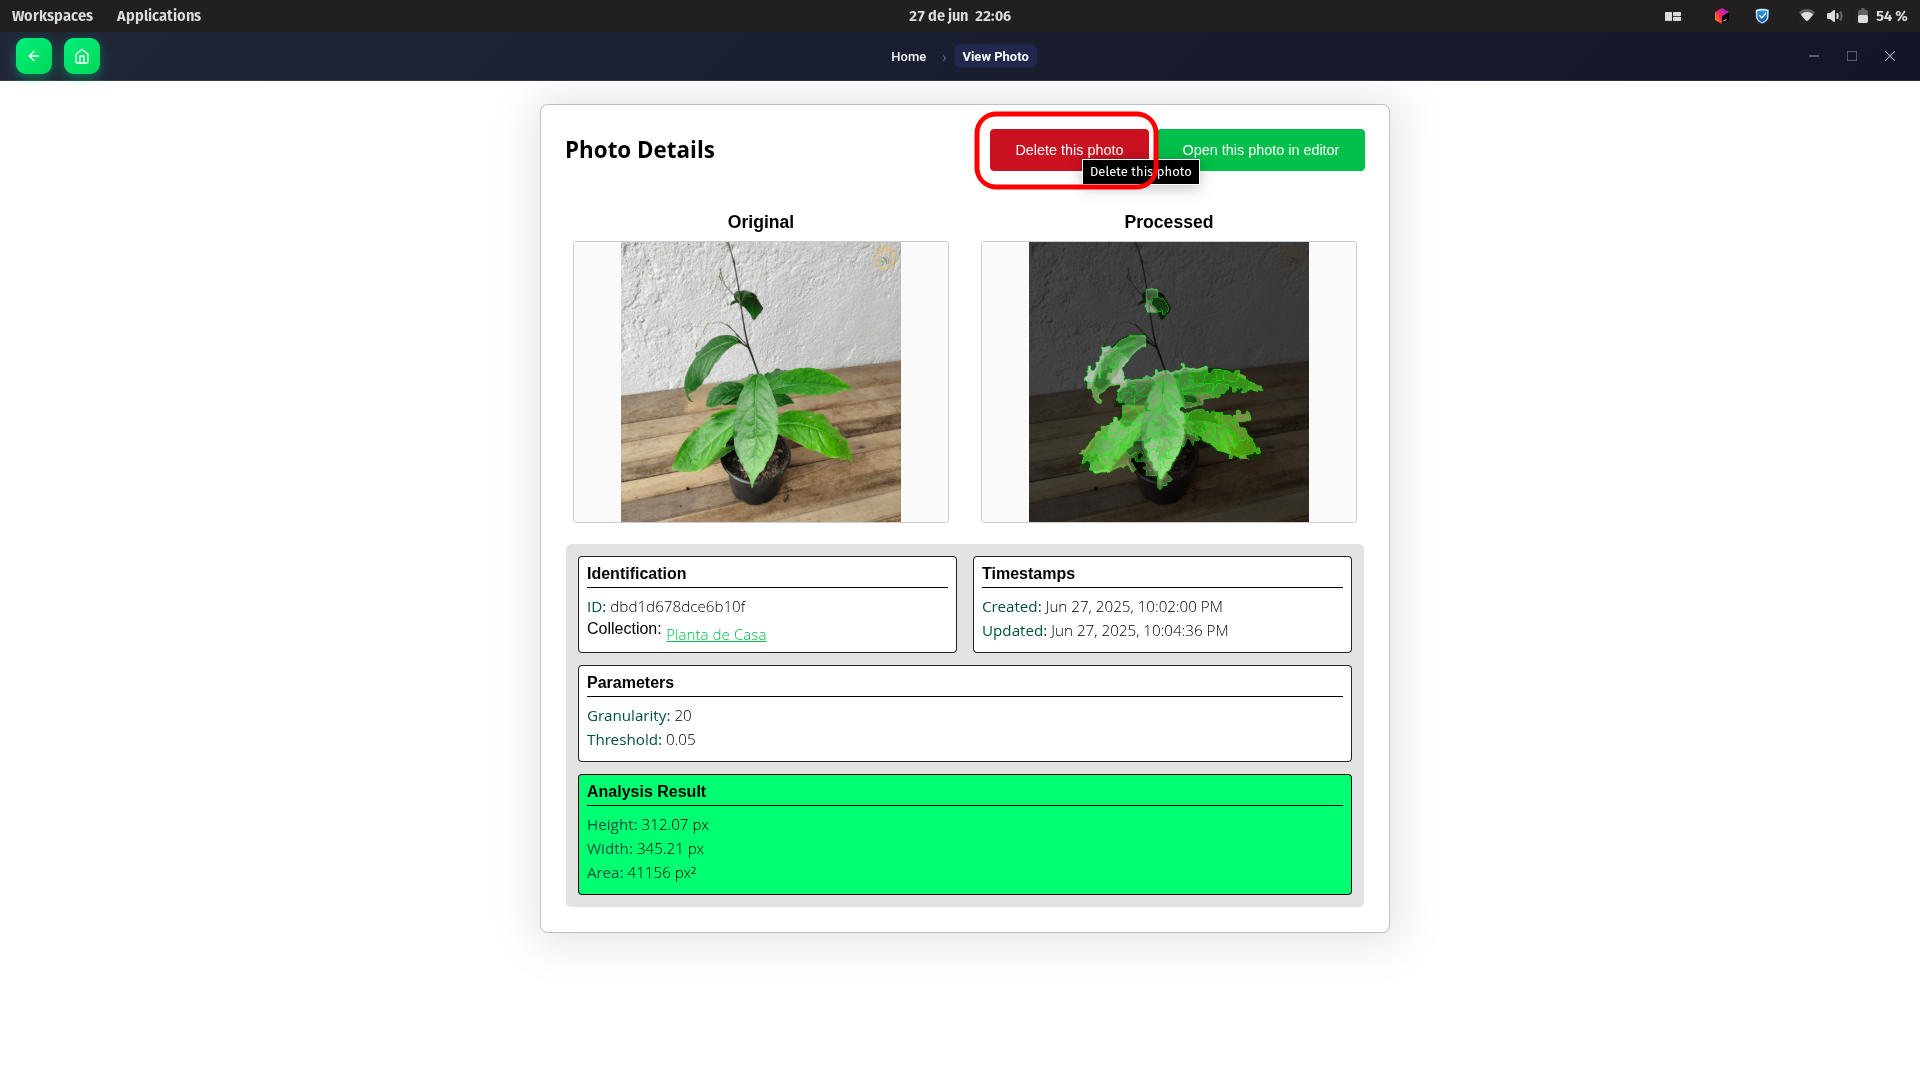
\includegraphics[width=1\textwidth]{../figures/screens/uc005/Screenshot from 2025-06-27 22-06-36.png}
    \caption{Selecionar opção de deletar foto. Fonte: os autores}
    \label{fig:uc005-screen2}
\end{figure}

\begin{figure}[H]
    \centering
    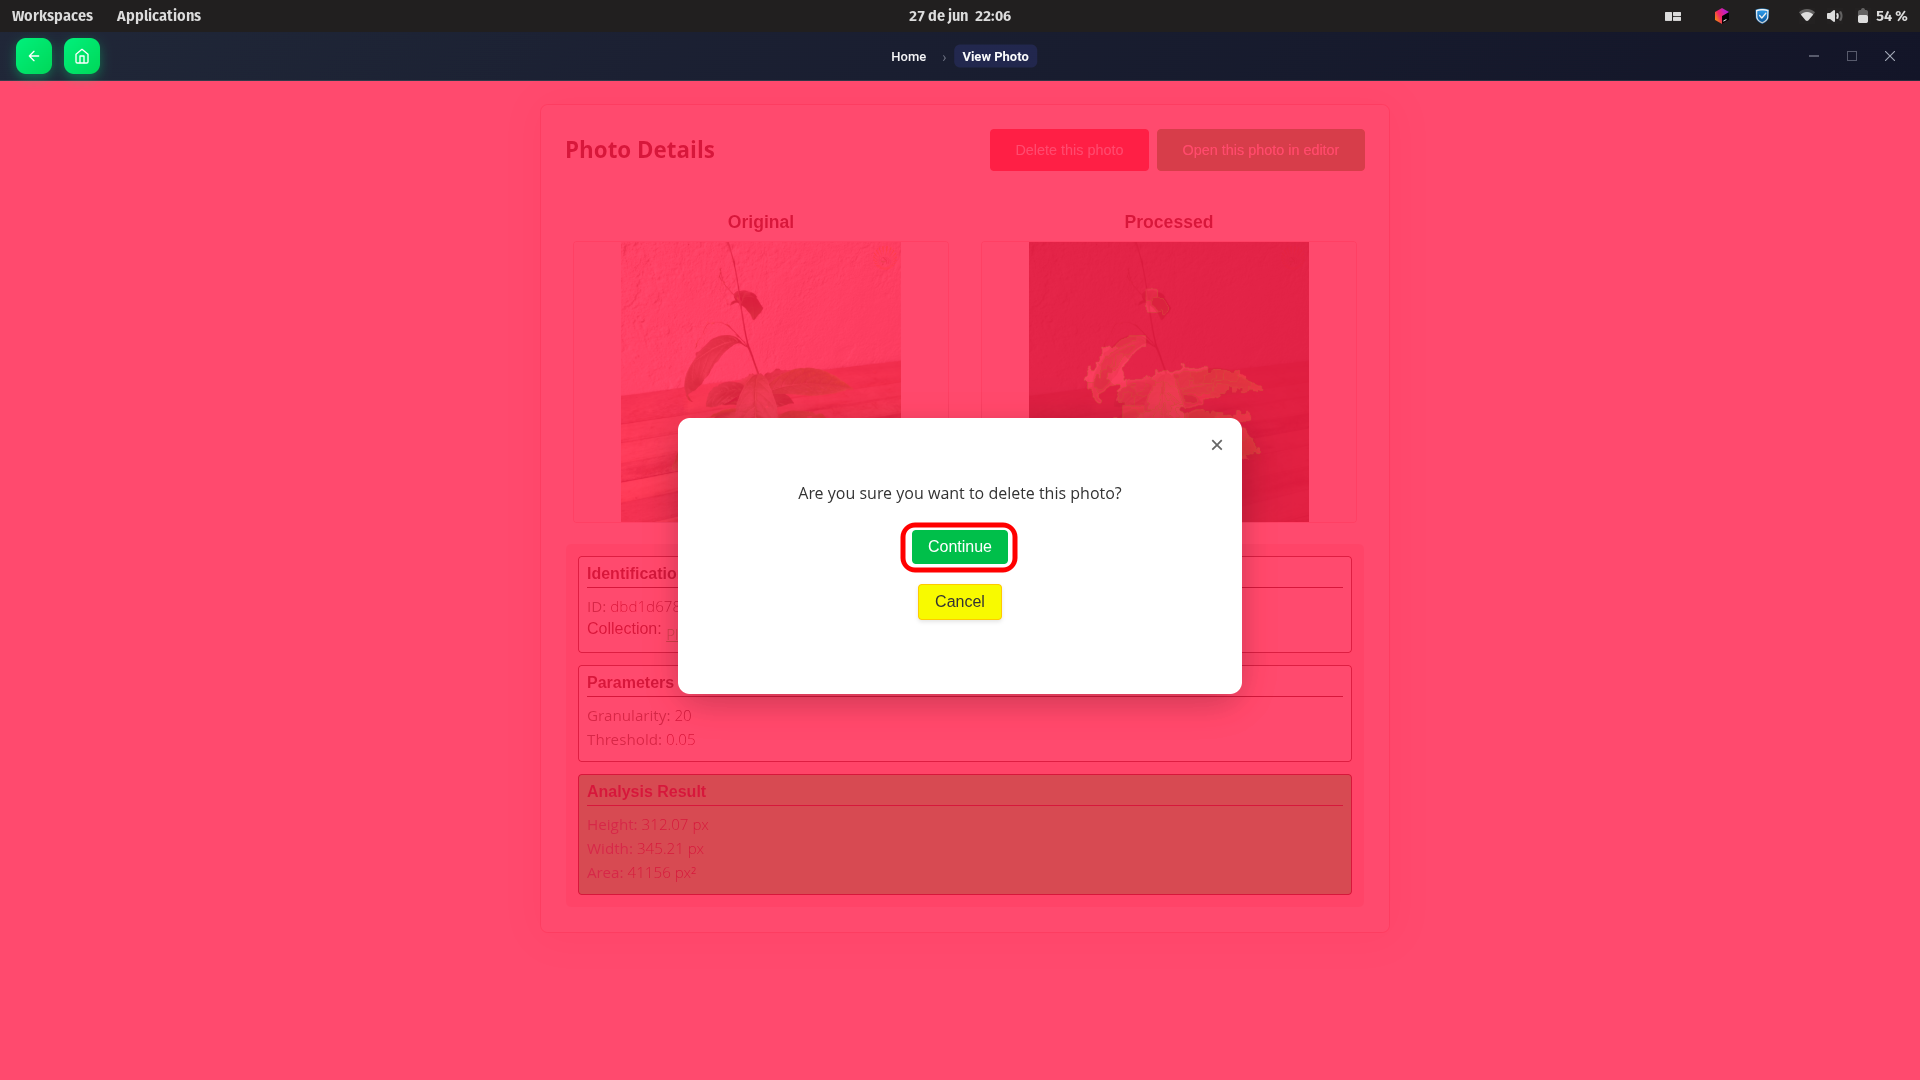
\includegraphics[width=1\textwidth]{../figures/screens/uc005/Screenshot from 2025-06-27 22-06-40.png}
    \caption{Confirmar ação. Fonte: os autores}
    \label{fig:uc005-screen3}
\end{figure}

\begin{figure}[H]
    \centering
    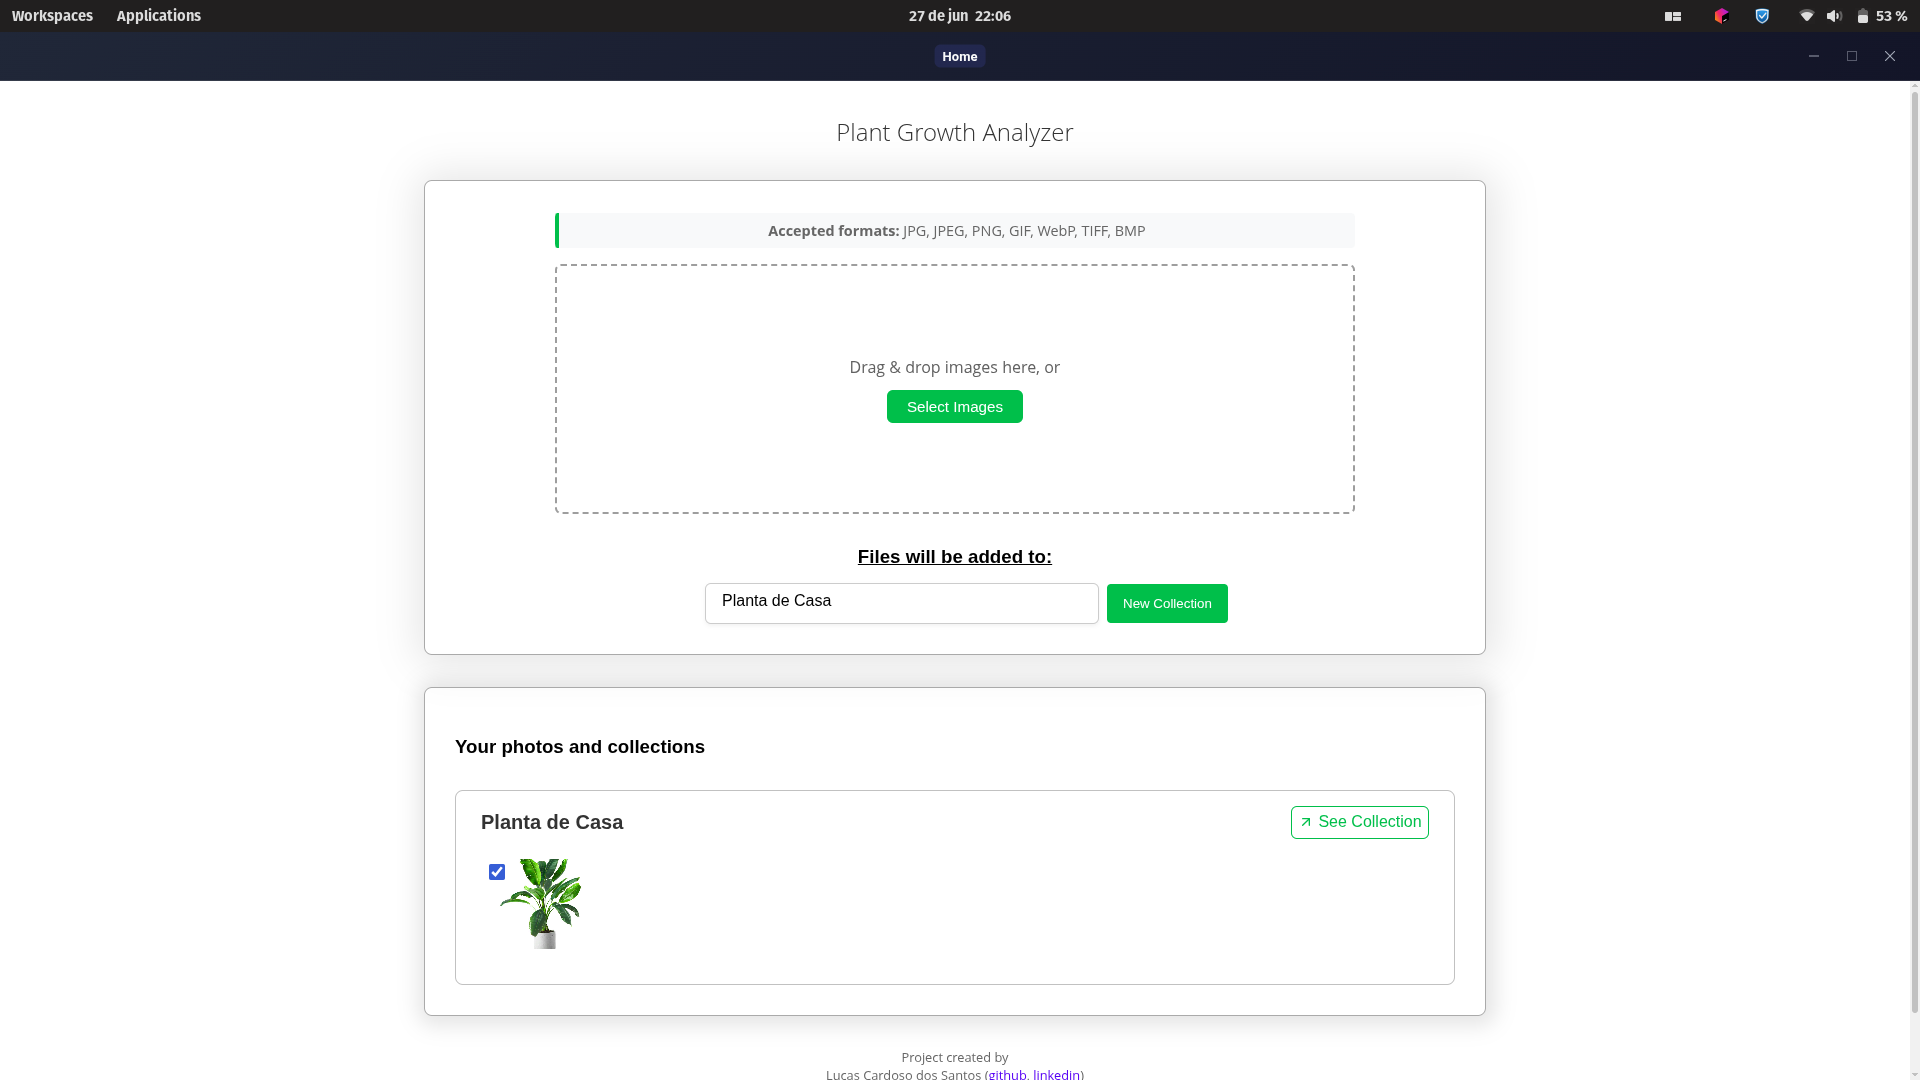
\includegraphics[width=1\textwidth]{../figures/screens/uc005/Screenshot from 2025-06-27 22-06-51.png}
    \caption{Foto deletada com sucesso. Fonte: os autores}
    \label{fig:uc005-screen4}
\end{figure}

\section{Visualizar detalhes de foto}

% TODO: Por que abrir em uma coleção???

\subsection{HTA Model}

\begin{figure}[H]
    \centering
    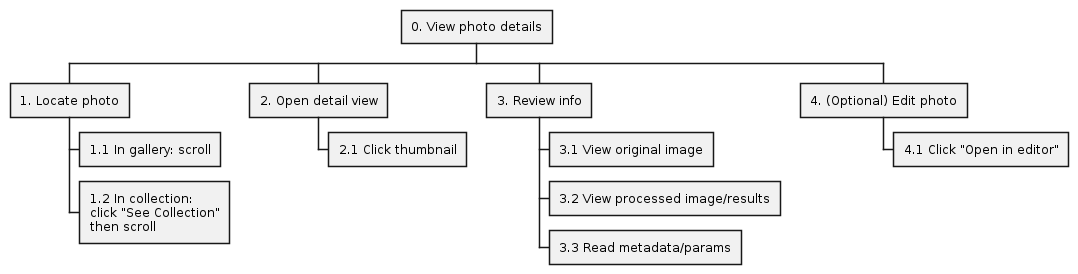
\includegraphics[width=0.9\textwidth]{../figures/hta/UC006.png}
    \caption{HTA Model para o caso de uso: Visualizar detalhes de foto. Fonte: os autores}
    \label{fig:hta-uc006}
\end{figure}

\subsection{Diagrama de Sequência}

\begin{figure}[H]
    \centering
    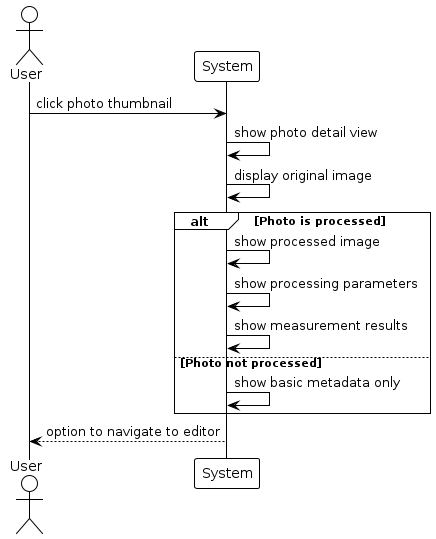
\includegraphics[width=0.9\textwidth]{../figures/dss/UC006.png}
    \caption{Diagrama de sequência para o caso de uso: Visualizar detalhes de foto. Fonte: os autores}
    \label{fig:dss-uc006}
\end{figure}

\subsection{Telas da Aplicação}

\begin{figure}[H]
    \centering
    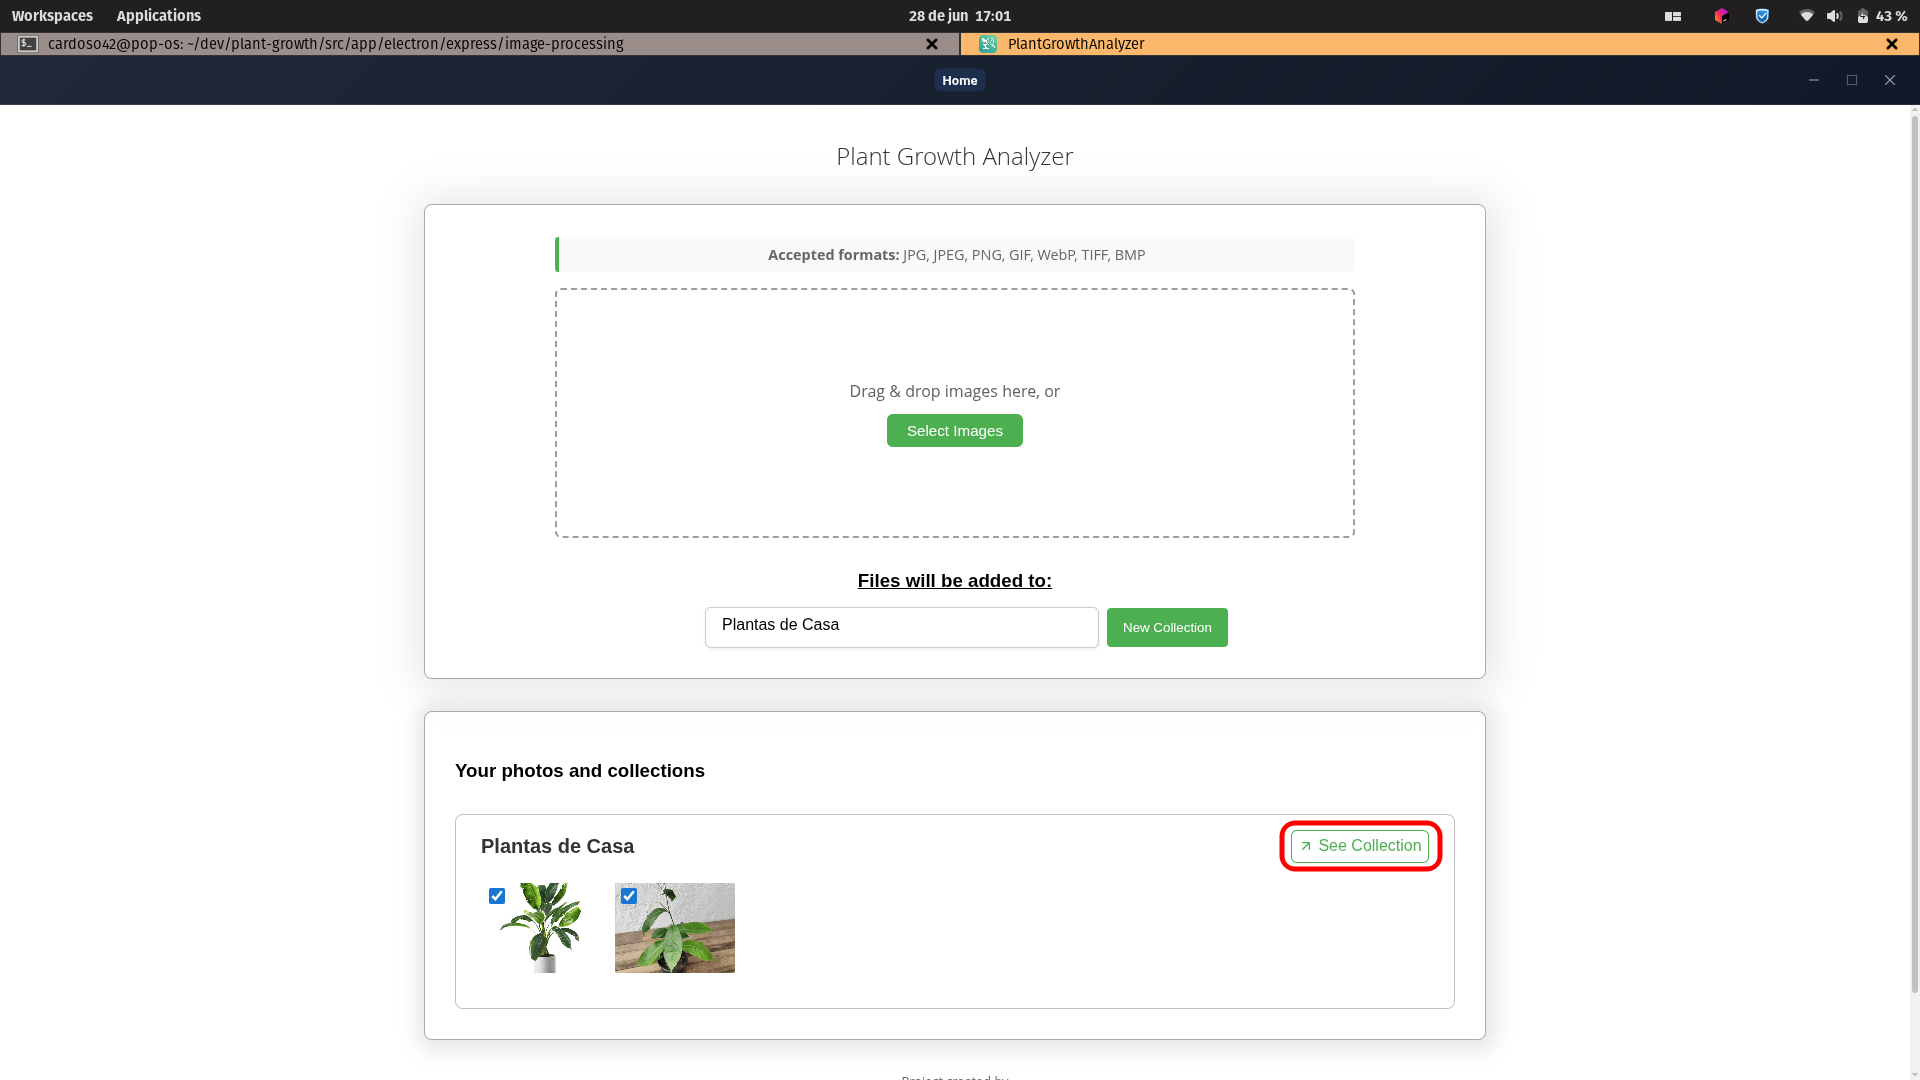
\includegraphics[width=1\textwidth]{../figures/screens/uc006/Screenshot from 2025-06-28 17-01-34.png}
    \caption{Abrir coleção. Fonte: os autores}
    \label{fig:uc006-screen1}
\end{figure}

\begin{figure}[H]
    \centering
    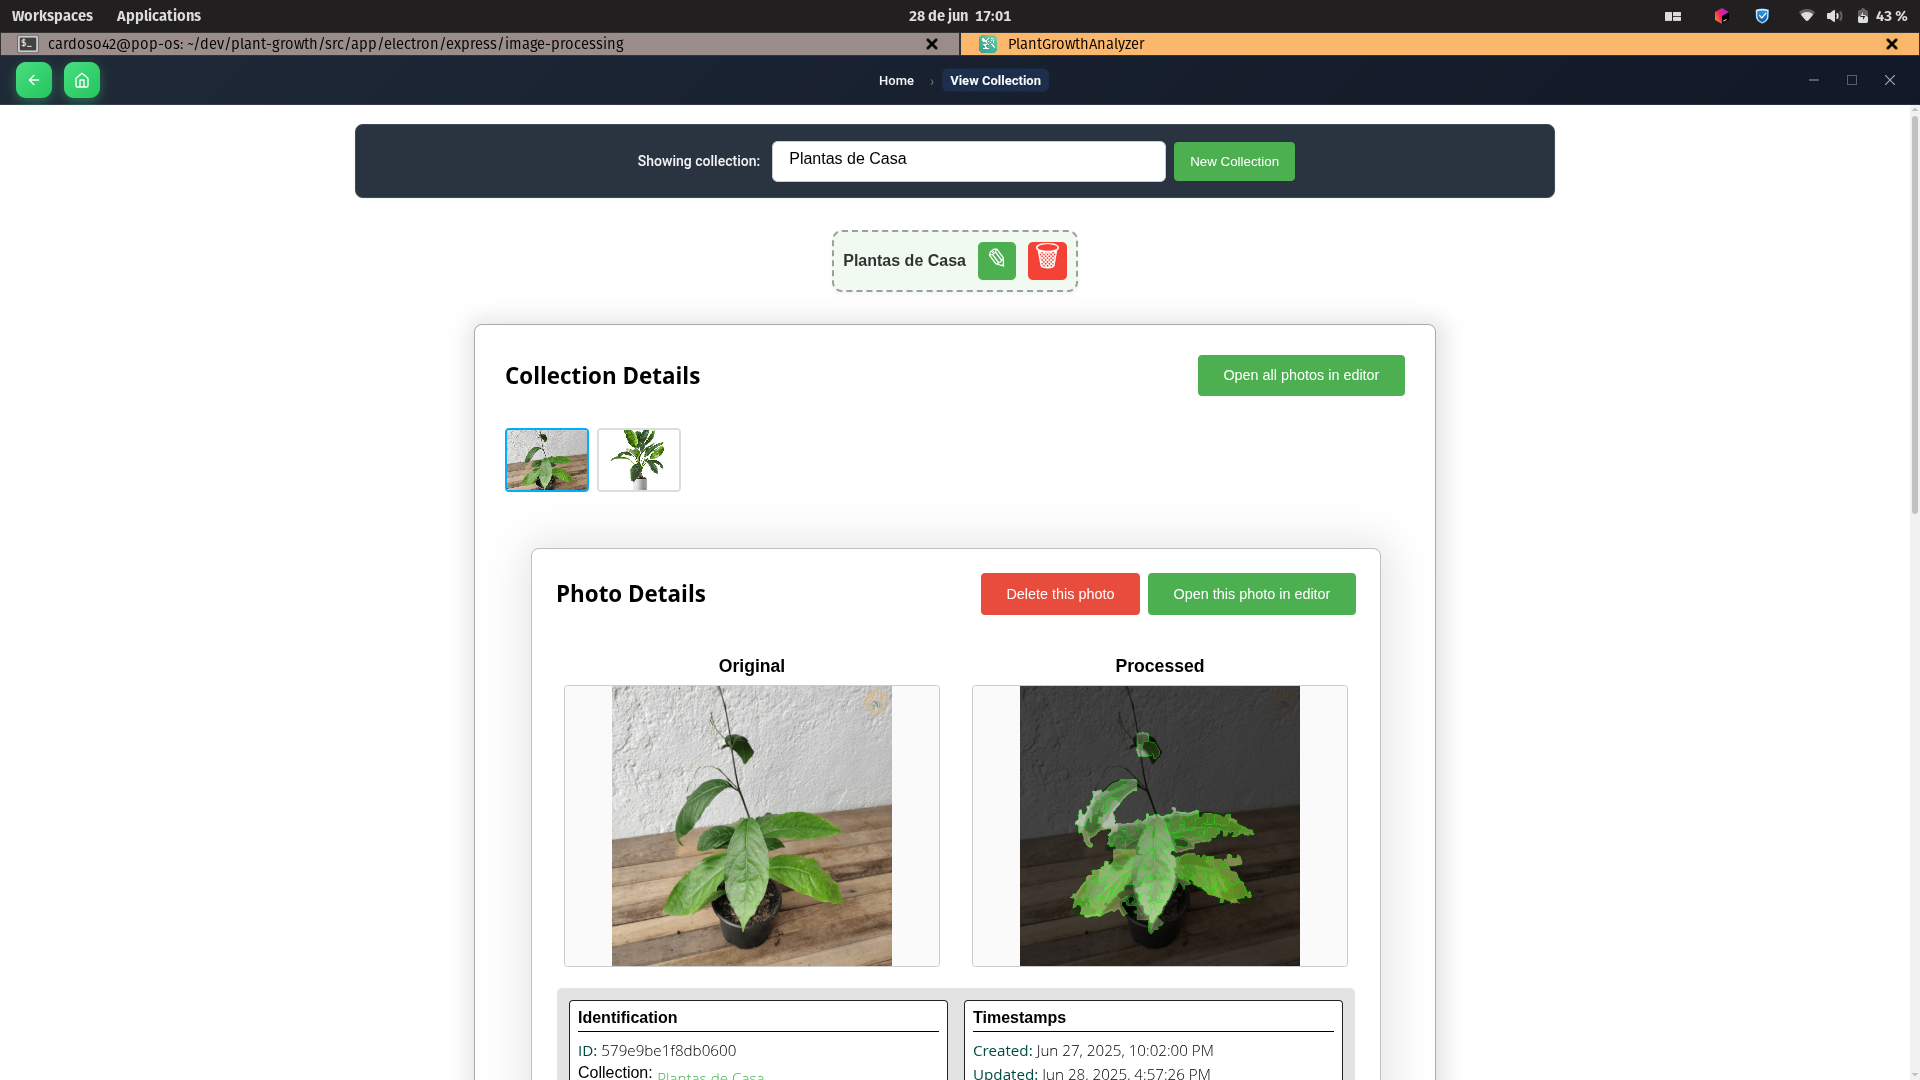
\includegraphics[width=1\textwidth]{../figures/screens/uc006/Screenshot from 2025-06-28 17-01-38.png}
    \caption{Tela de visualização da imagem dentro da coleção. Fonte: os autores}
    \label{fig:uc006-screen2}
\end{figure}

\begin{figure}[H]
    \centering
    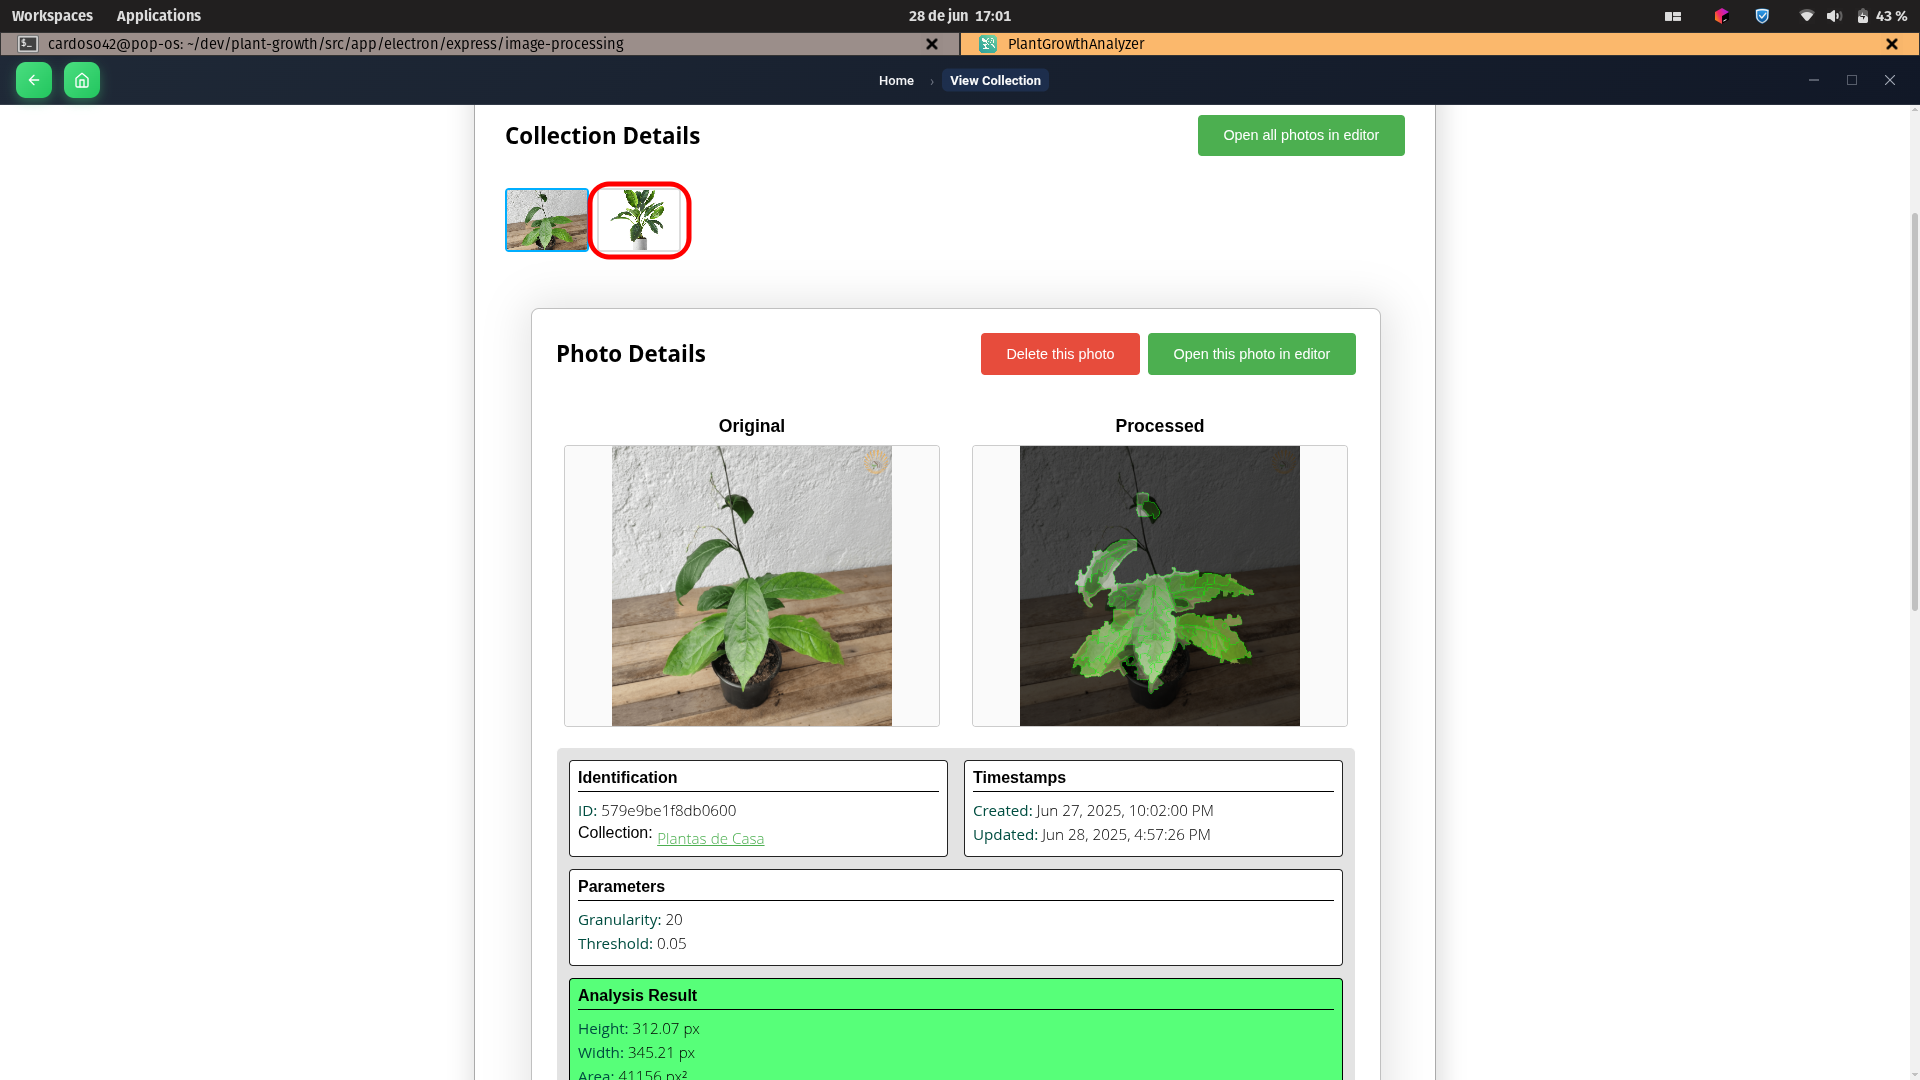
\includegraphics[width=1\textwidth]{../figures/screens/uc006/Screenshot from 2025-06-28 17-01-45.png}
    \caption{Visualização estendida e possibilidade de ver outras imagens. Fonte: os autores}
    \label{fig:uc006-screen3}
\end{figure}

\begin{figure}[H]
    \centering
    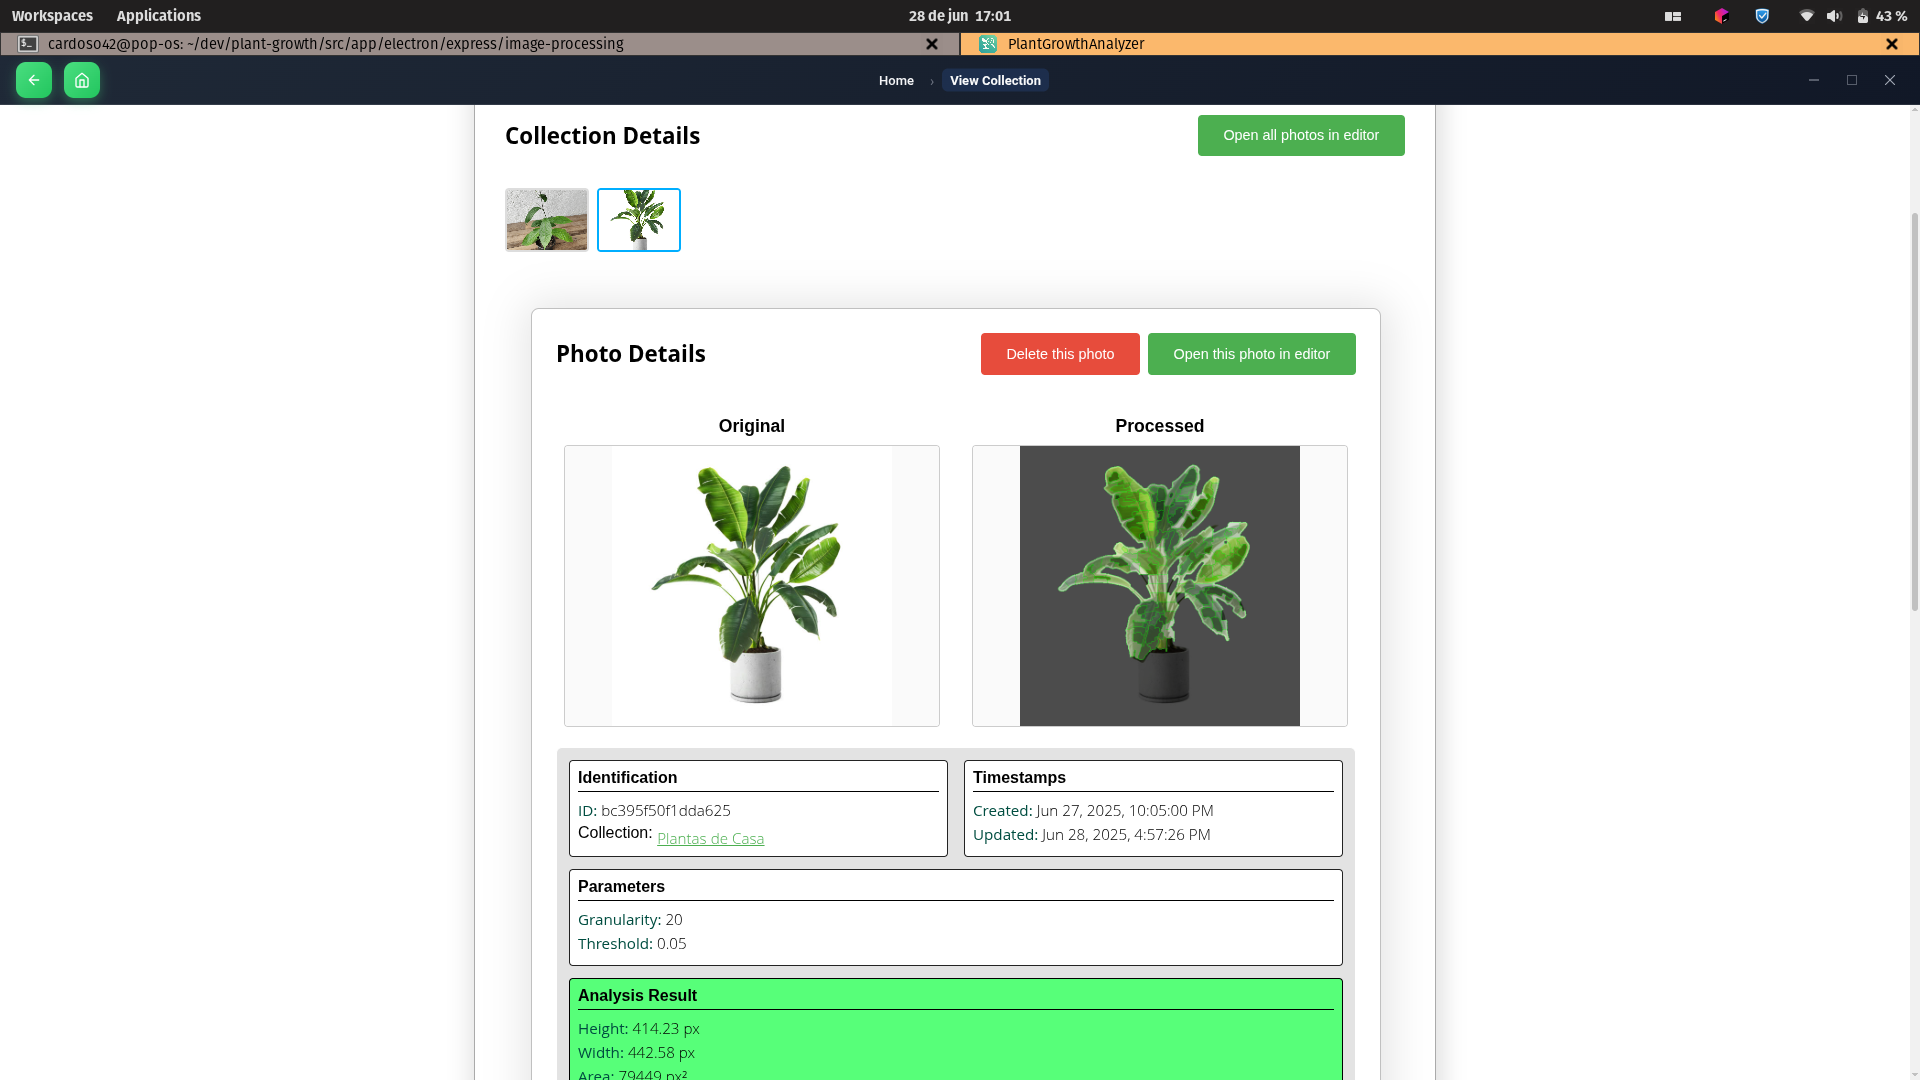
\includegraphics[width=1\textwidth]{../figures/screens/uc006/Screenshot from 2025-06-28 17-01-48.png}
    \caption{Visualização das imagens de outra foto. Fonte: os autores}
    \label{fig:uc006-screen4}
\end{figure}

\begin{figure}[H]
    \centering
    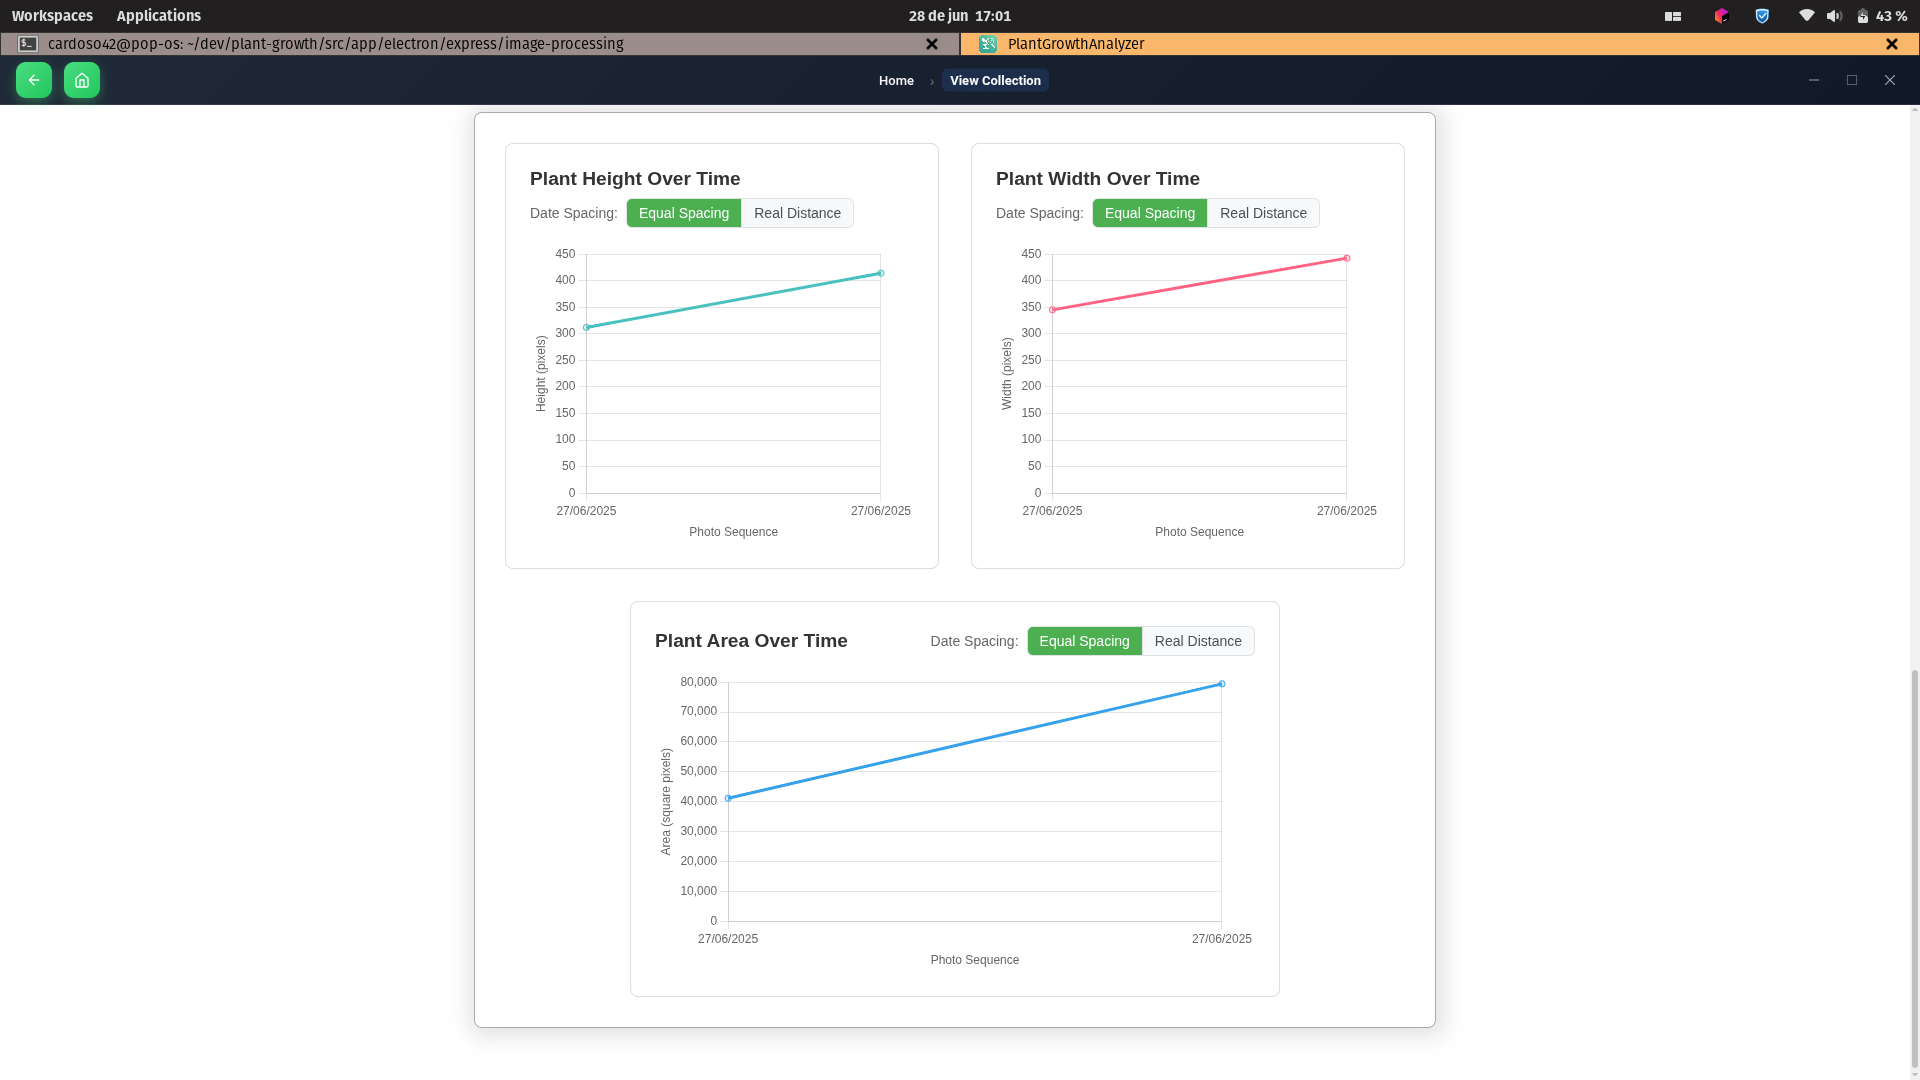
\includegraphics[width=1\textwidth]{../figures/screens/uc006/Screenshot from 2025-06-28 17-01-54.png}
    \caption{Gráficos comparativos. Fonte: os autores}
    \label{fig:uc006-screen5}
\end{figure}

\section{Criar nova coleção}

\subsection{HTA Model}

\begin{figure}[H]
    \centering
    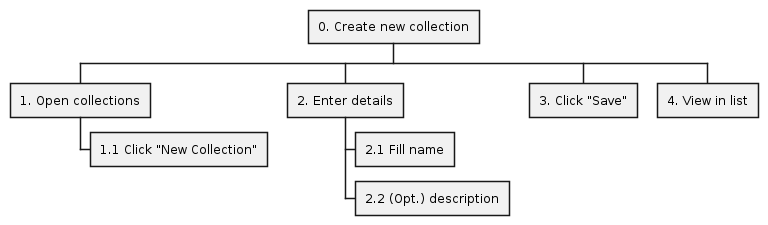
\includegraphics[width=0.9\textwidth]{../figures/hta/UC007.png}
    \caption{HTA Model para o caso de uso: Criar nova coleção. Fonte: os autores}
    \label{fig:hta-uc007}
\end{figure}

\subsection{Diagrama de Sequência}

\begin{figure}[H]
    \centering
    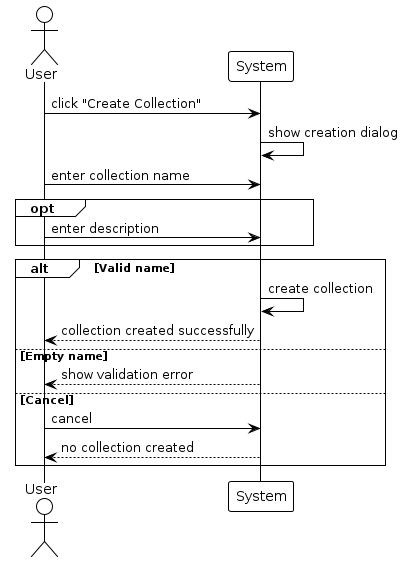
\includegraphics[width=0.9\textwidth]{../figures/dss/UC007.png}
    \caption{Diagrama de sequência para o caso de uso: Criar nova coleção. Fonte: os autores}
    \label{fig:dss-uc007}
\end{figure}

\subsection{Telas da Aplicação}

\begin{figure}[H]
    \centering
    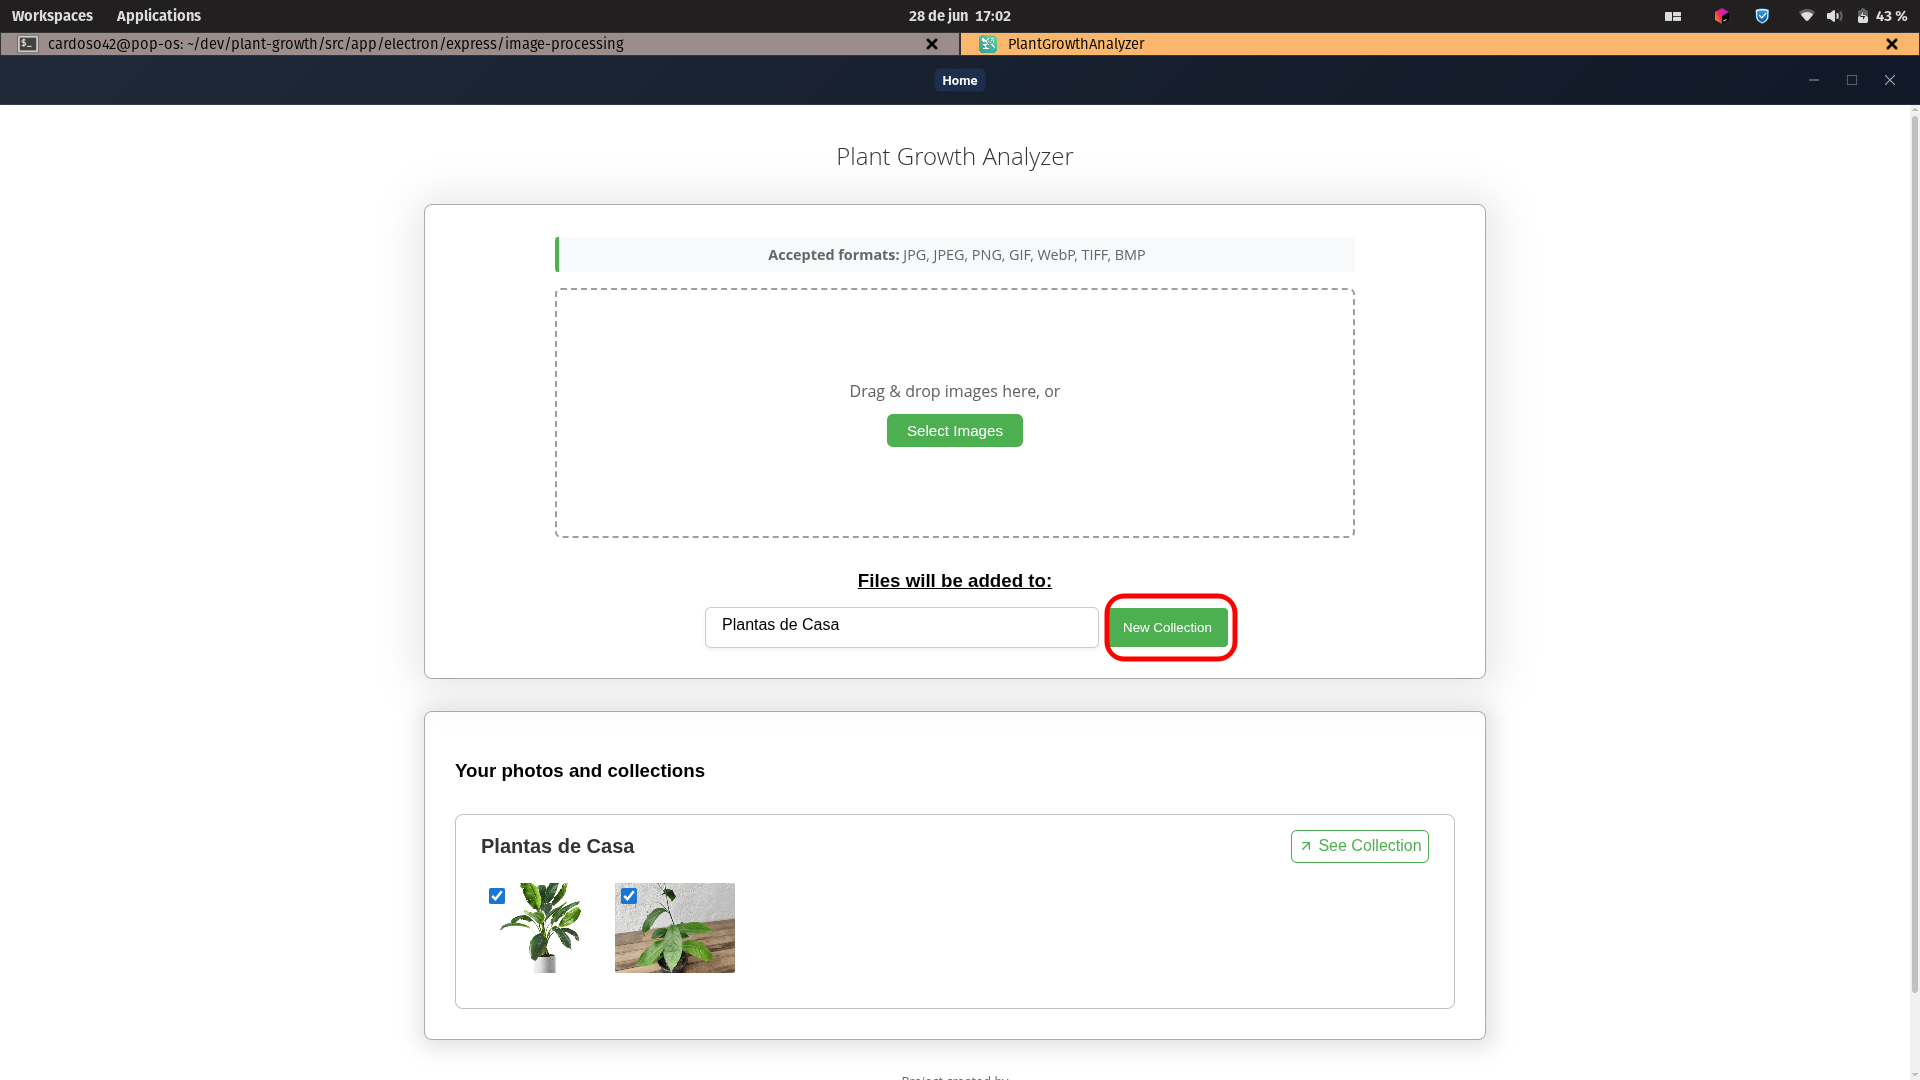
\includegraphics[width=1\textwidth]{../figures/screens/uc007/Screenshot from 2025-06-28 17-02-44.png}
    \caption{Tela inicial para criar nova coleção. Fonte: os autores}
    \label{fig:uc007-screen1}
\end{figure}

\begin{figure}[H]
    \centering
    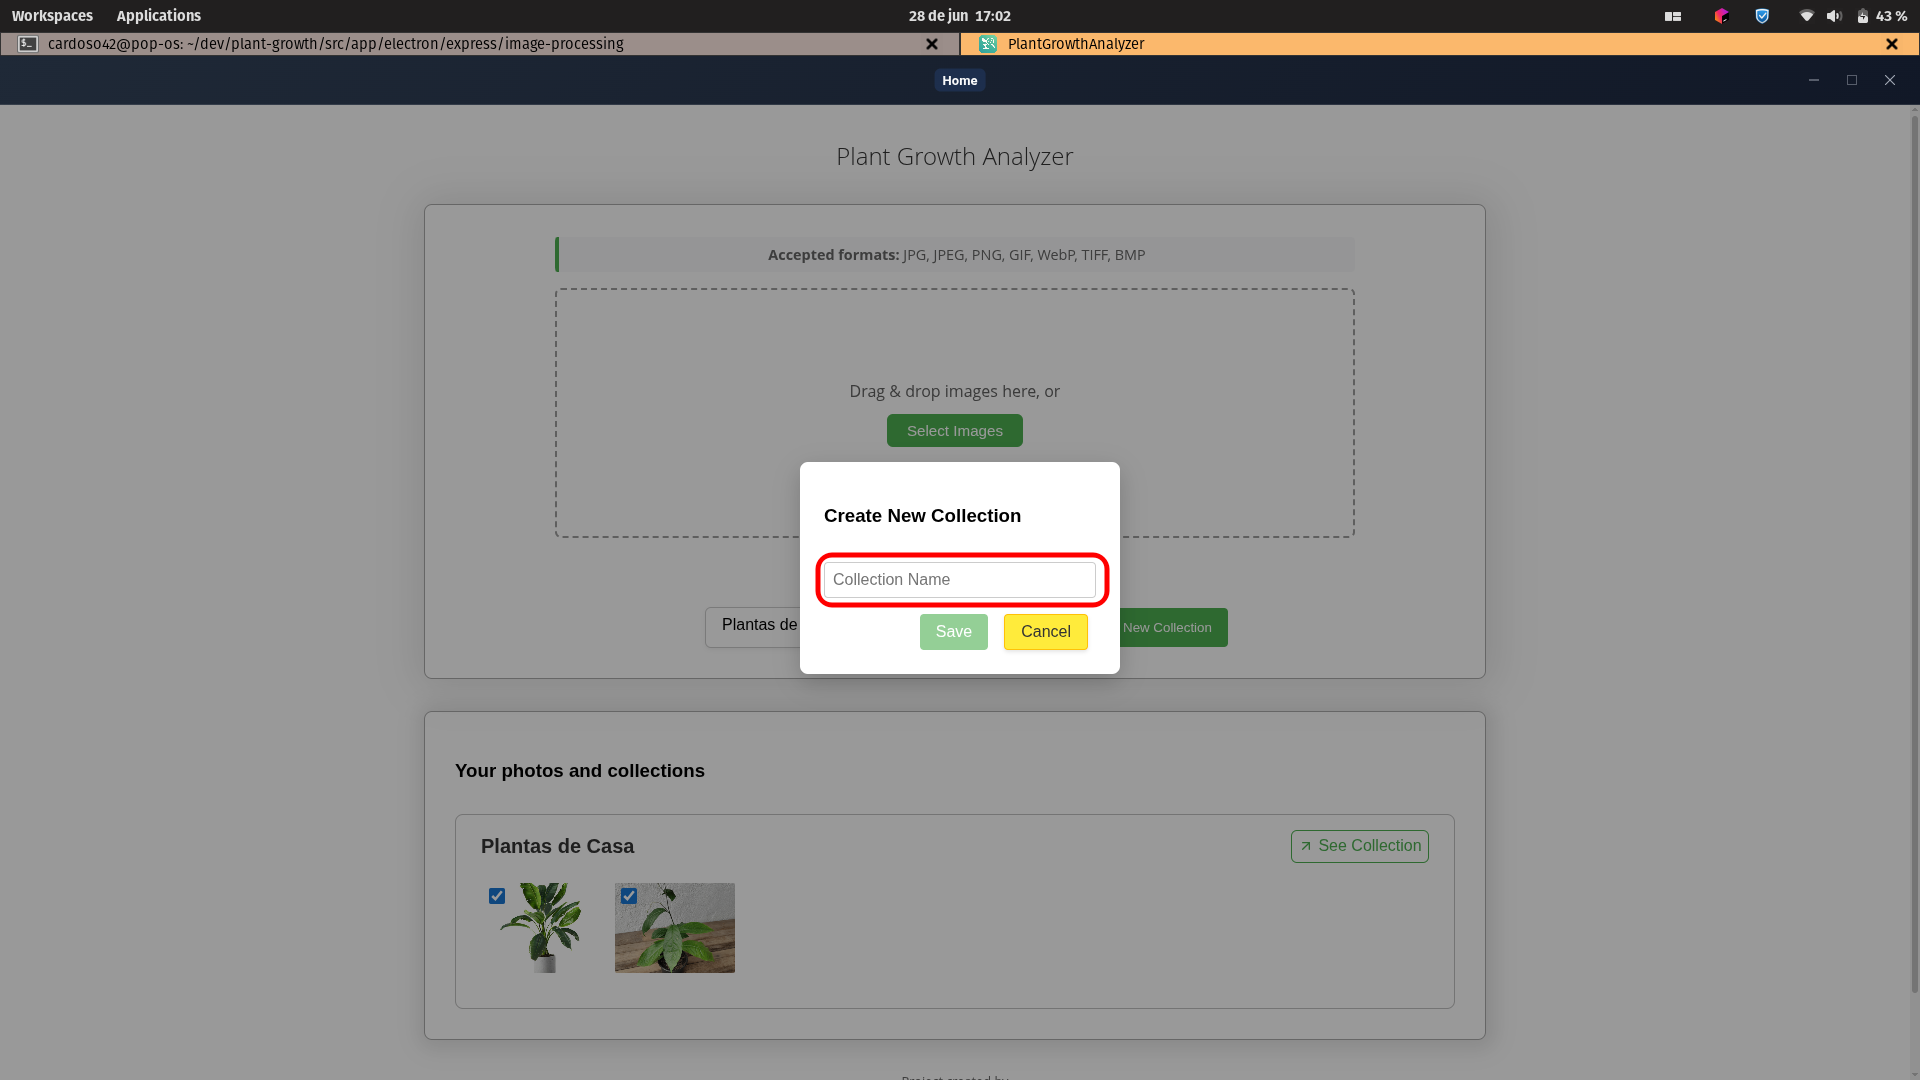
\includegraphics[width=1\textwidth]{../figures/screens/uc007/Screenshot from 2025-06-28 17-02-47.png}
    \caption{Formulário de criação de coleção. Fonte: os autores}
    \label{fig:uc007-screen2}
\end{figure}

\begin{figure}[H]
    \centering
    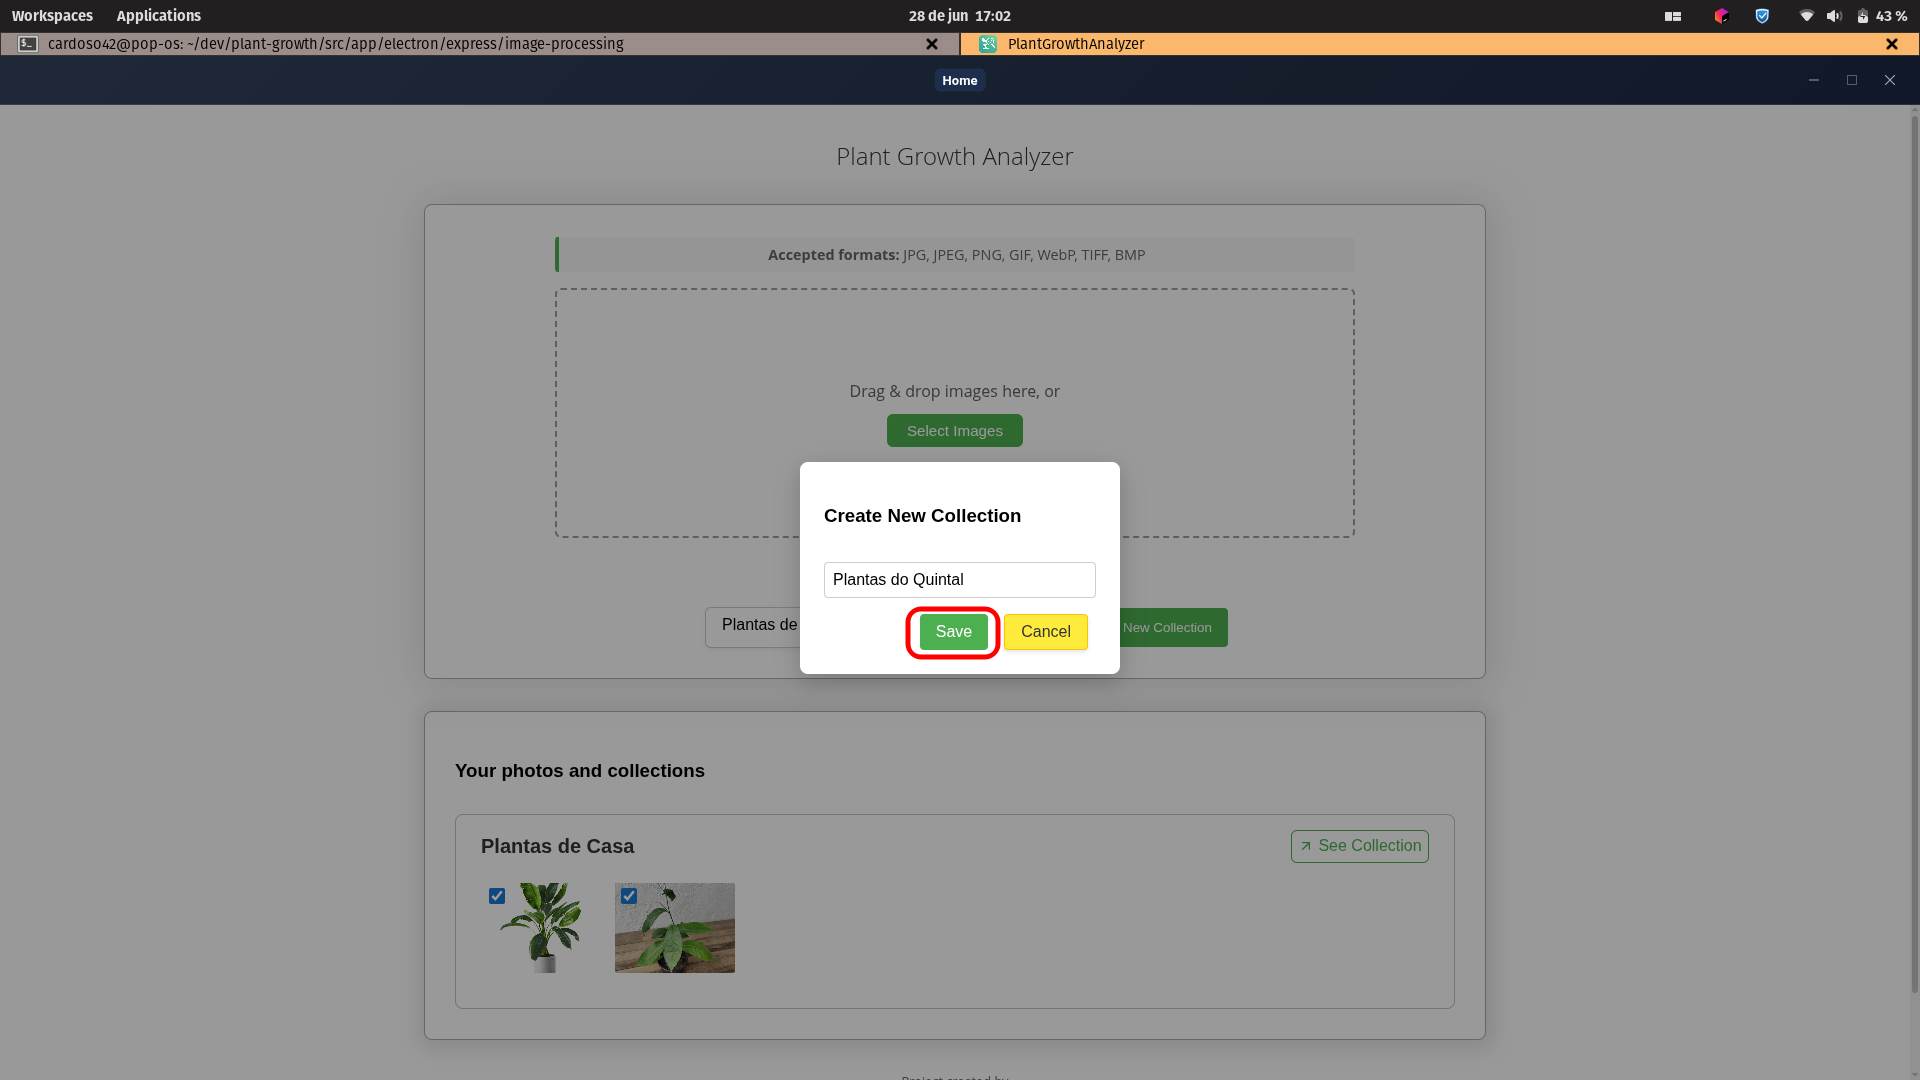
\includegraphics[width=1\textwidth]{../figures/screens/uc007/Screenshot from 2025-06-28 17-02-56.png}
    \caption{Preenchimento do nome da coleção. Fonte: os autores}
    \label{fig:uc007-screen3}
\end{figure}

\begin{figure}[H]
    \centering
    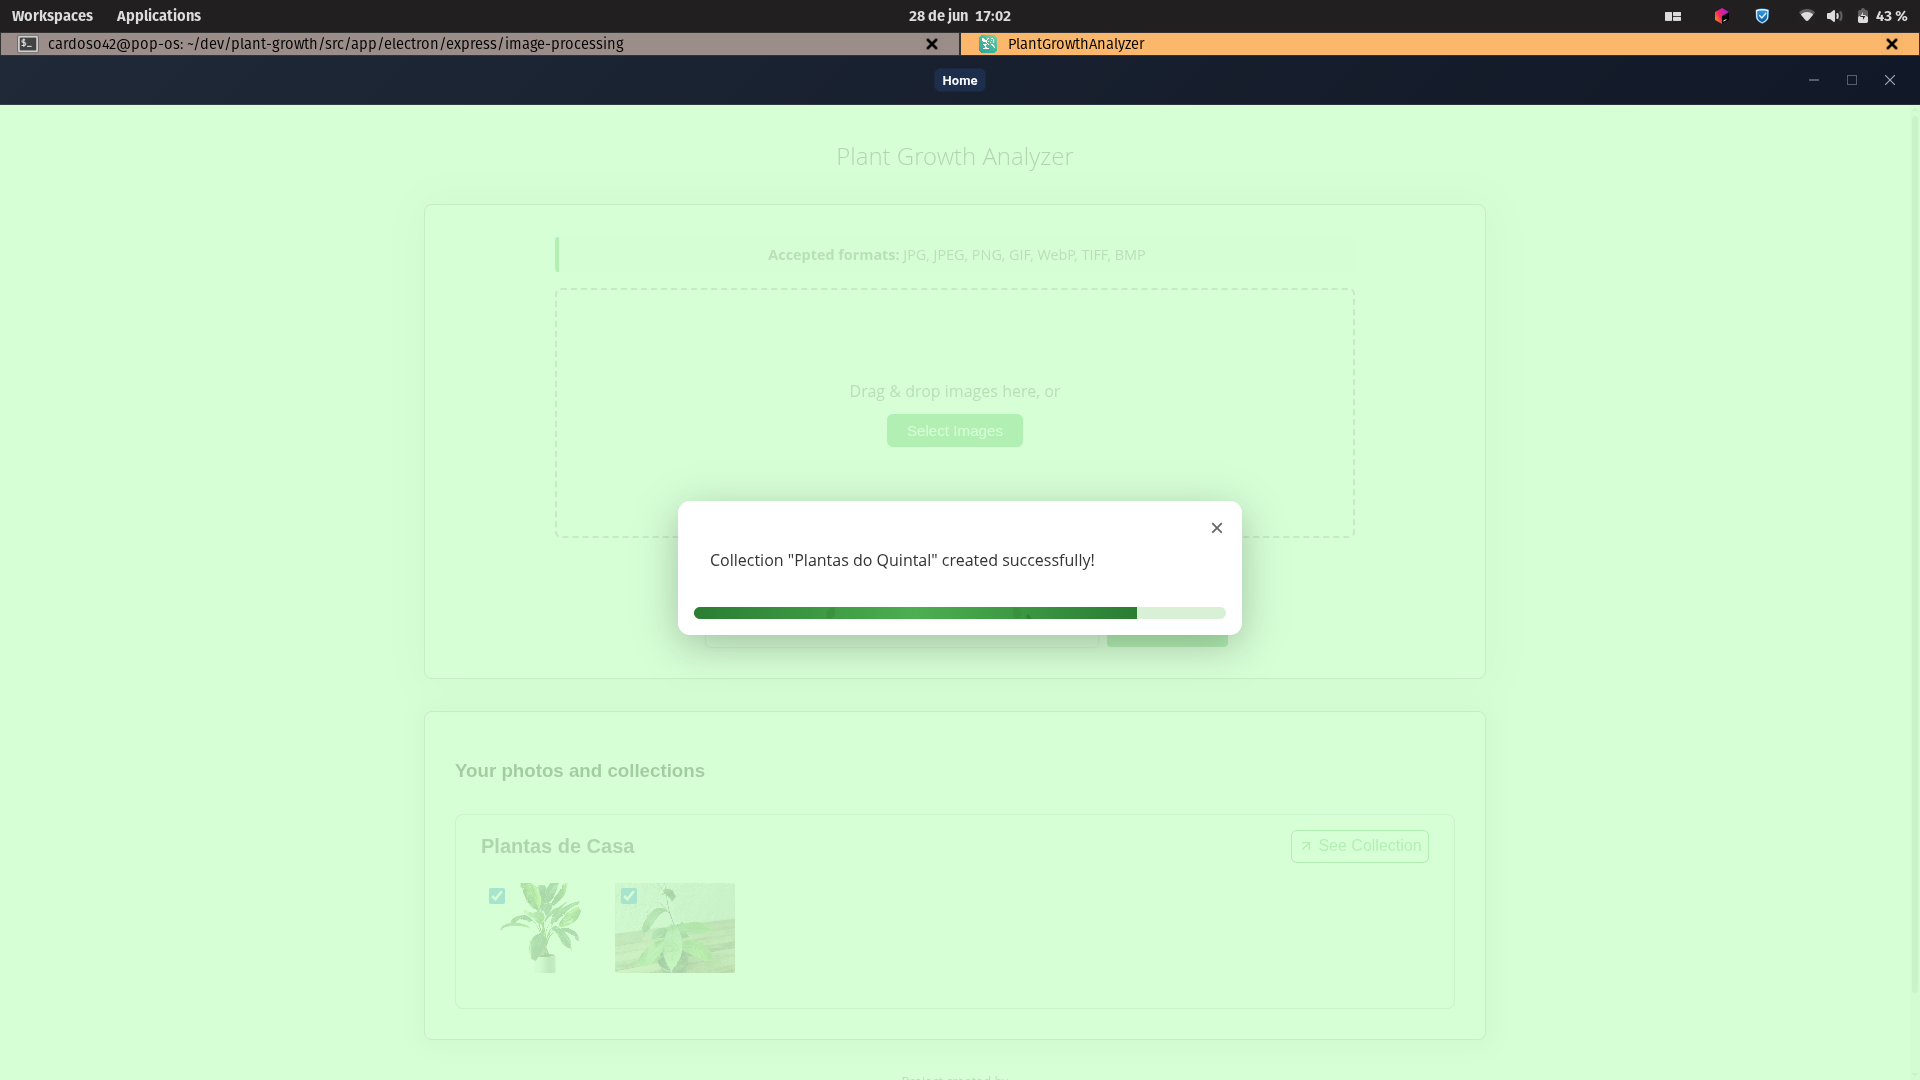
\includegraphics[width=1\textwidth]{../figures/screens/uc007/Screenshot from 2025-06-28 17-03-00.png}
    \caption{Confirmação da criação. Fonte: os autores}
    \label{fig:uc007-screen4}
\end{figure}

\begin{figure}[H]
    \centering
    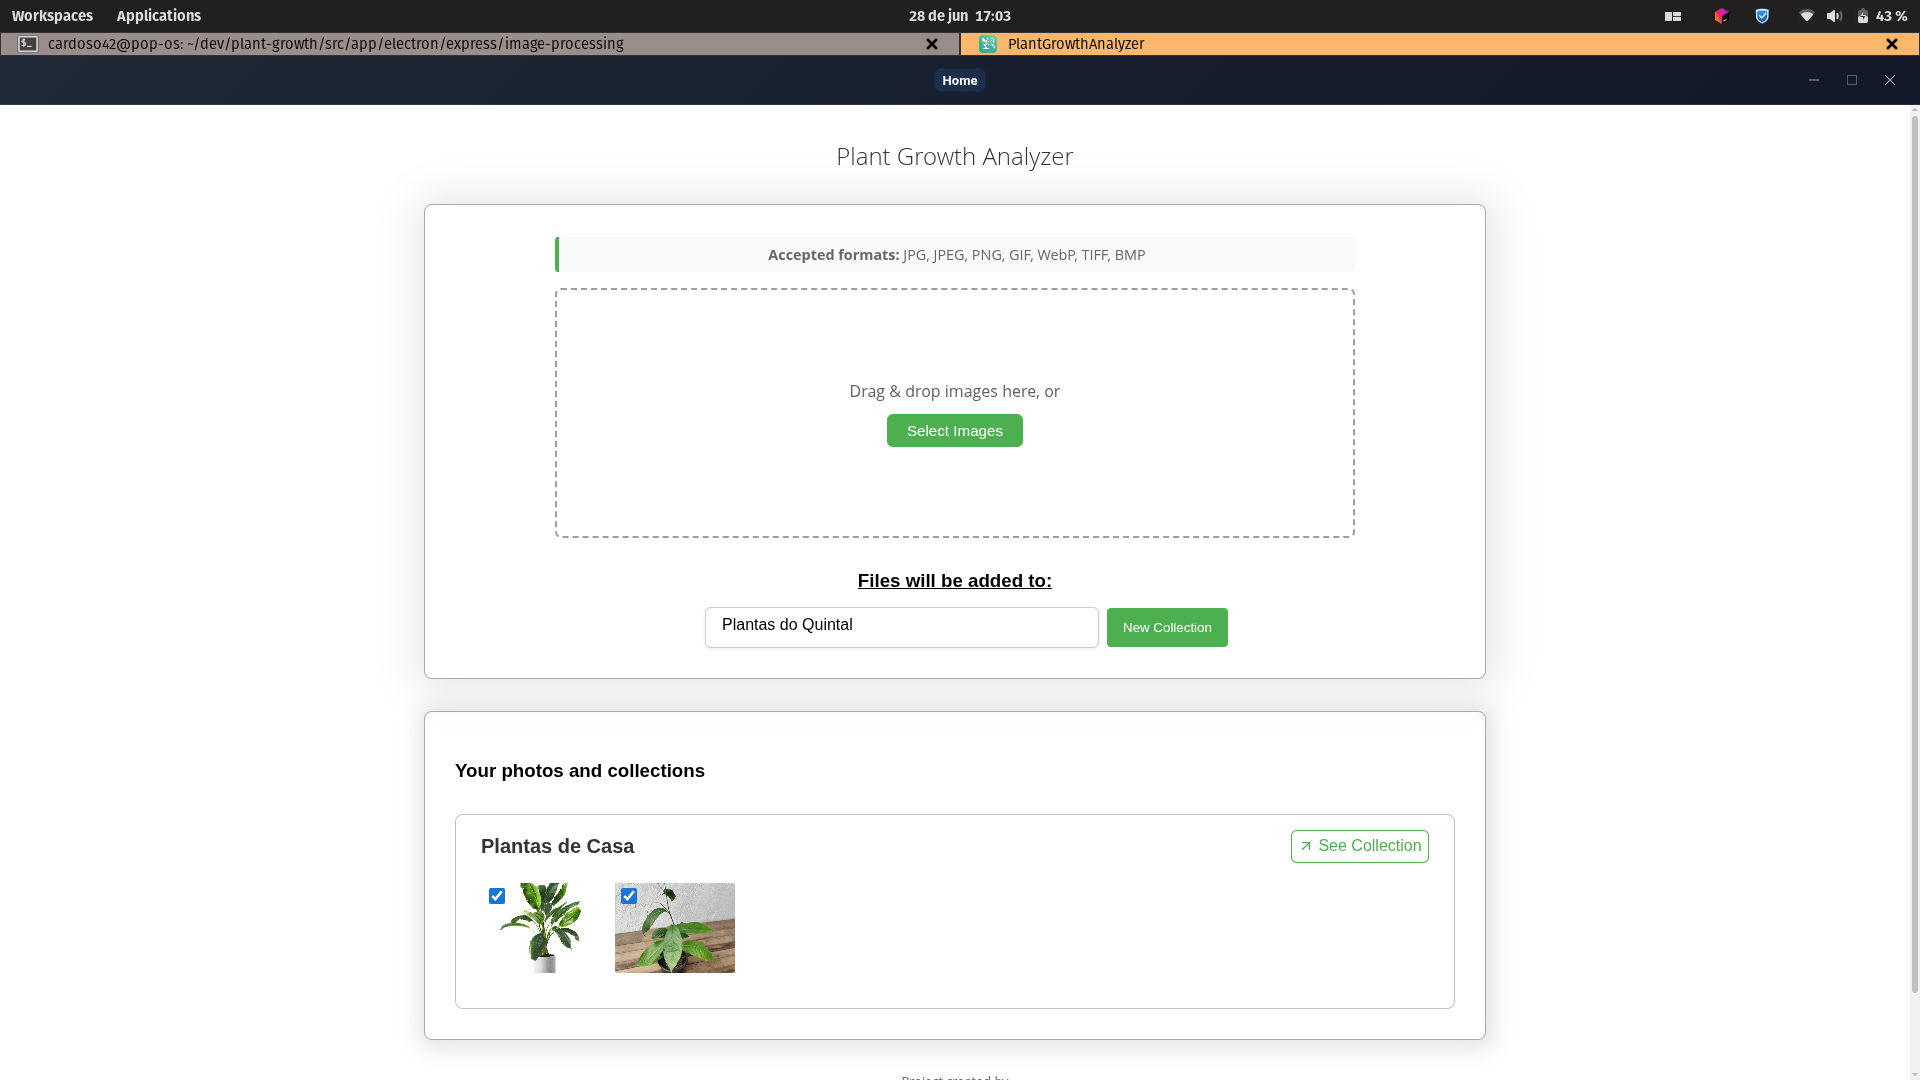
\includegraphics[width=1\textwidth]{../figures/screens/uc007/Screenshot from 2025-06-28 17-03-57.png}
    \caption{Coleção criada com sucesso. Fonte: os autores}
    \label{fig:uc007-screen5}
\end{figure}

\section{Renomear coleção}

\subsection{HTA Model}

\begin{figure}[H]
    \centering
    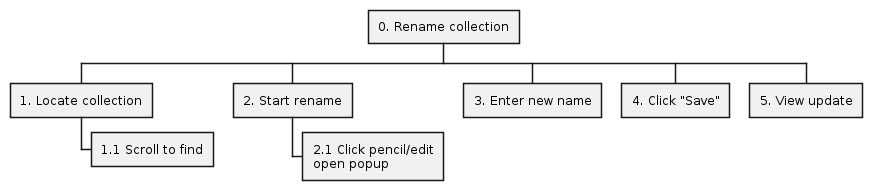
\includegraphics[width=0.9\textwidth]{../figures/hta/UC008.png}
    \caption{HTA Model para o caso de uso: Renomear coleção. Fonte: os autores}
    \label{fig:hta-uc008}
\end{figure}

\subsection{Diagrama de Sequência}

\begin{figure}[H]
    \centering
    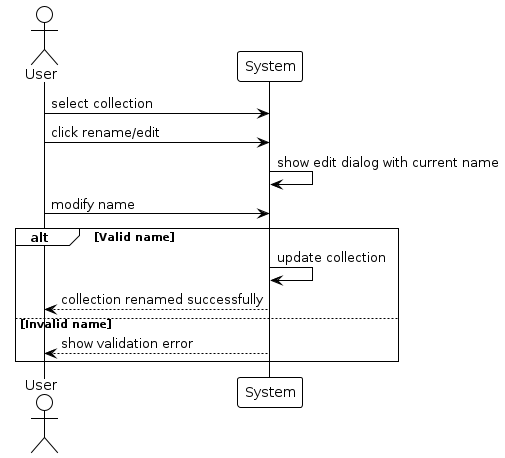
\includegraphics[width=0.9\textwidth]{../figures/dss/UC008.png}
    \caption{Diagrama de sequência para o caso de uso: Renomear coleção. Fonte: os autores}
    \label{fig:dss-uc008}
\end{figure}

\subsection{Telas da Aplicação}

\begin{figure}[H]
    \centering
    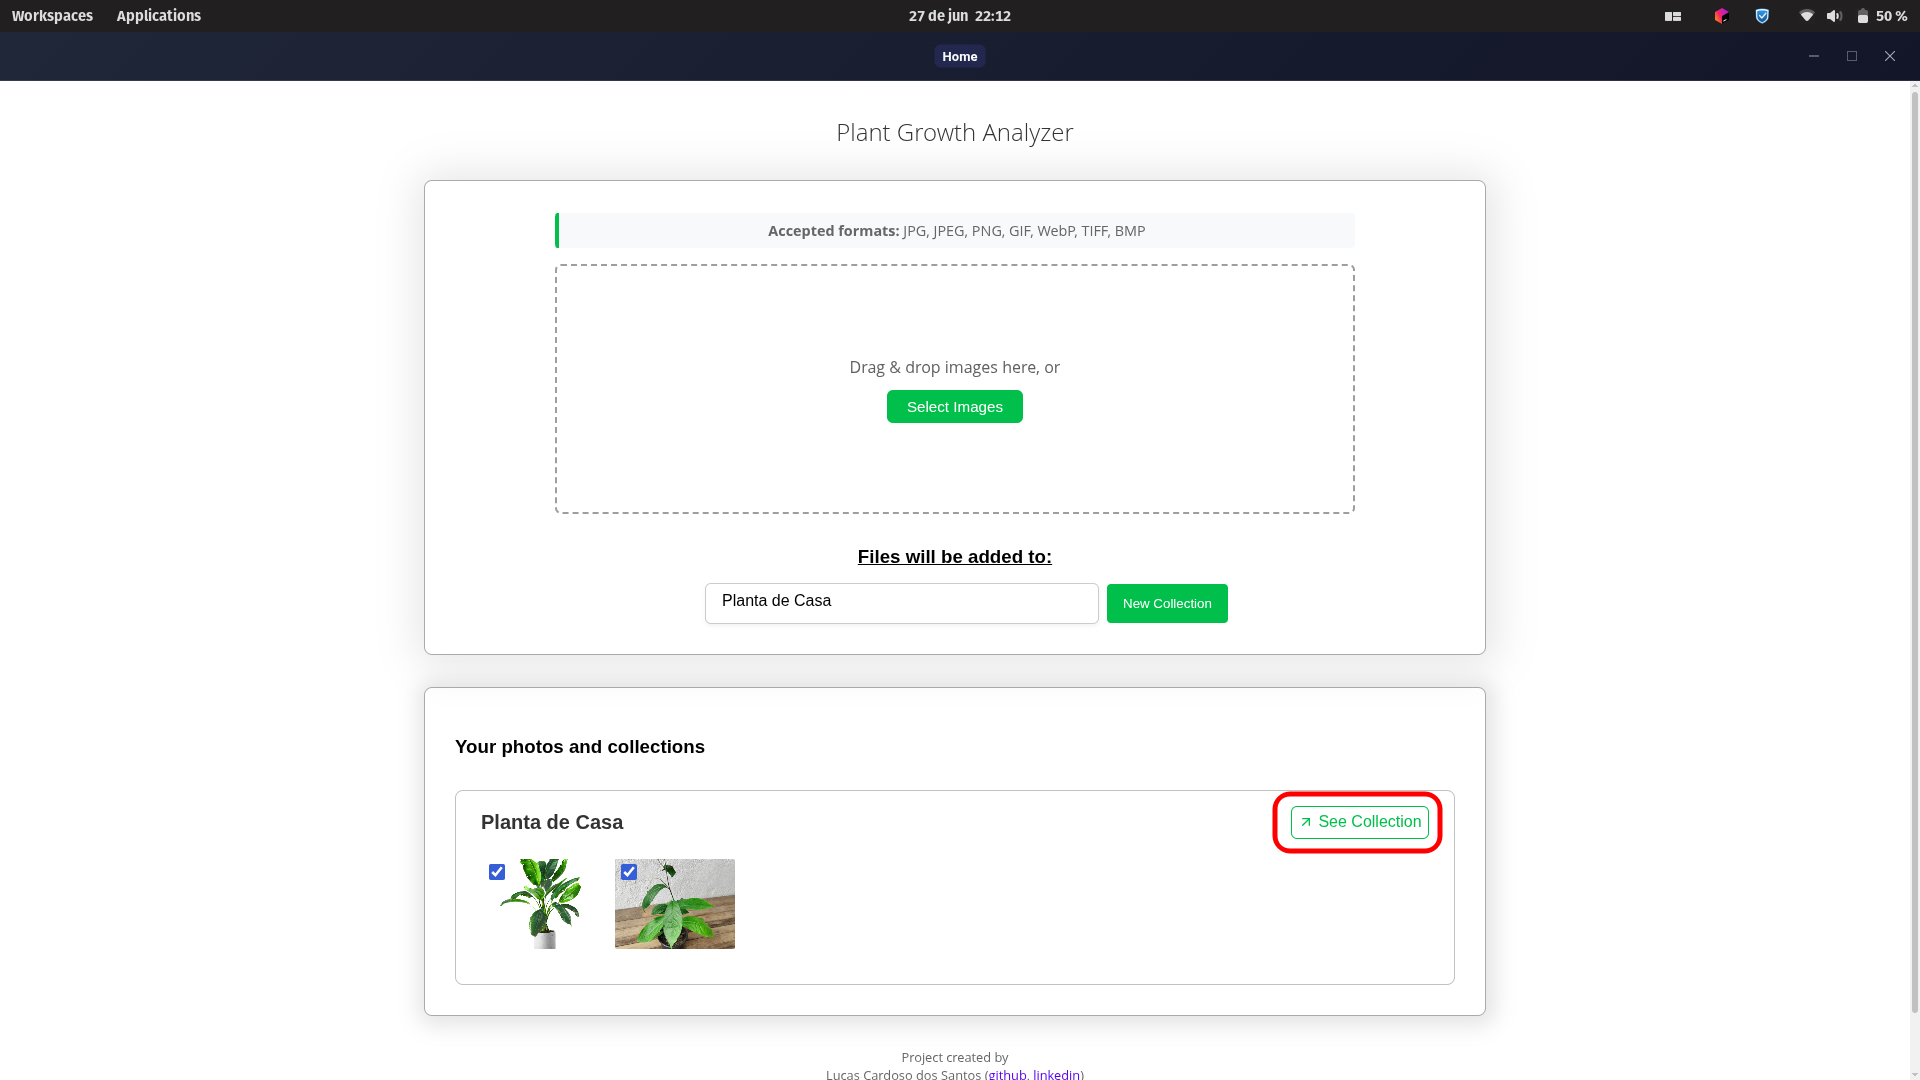
\includegraphics[width=1\textwidth]{../figures/screens/uc008/Screenshot from 2025-06-27 22-12-41.png}
    \caption{Tela inicial para renomear coleção. Fonte: os autores}
    \label{fig:uc008-screen1}
\end{figure}

\begin{figure}[H]
    \centering
    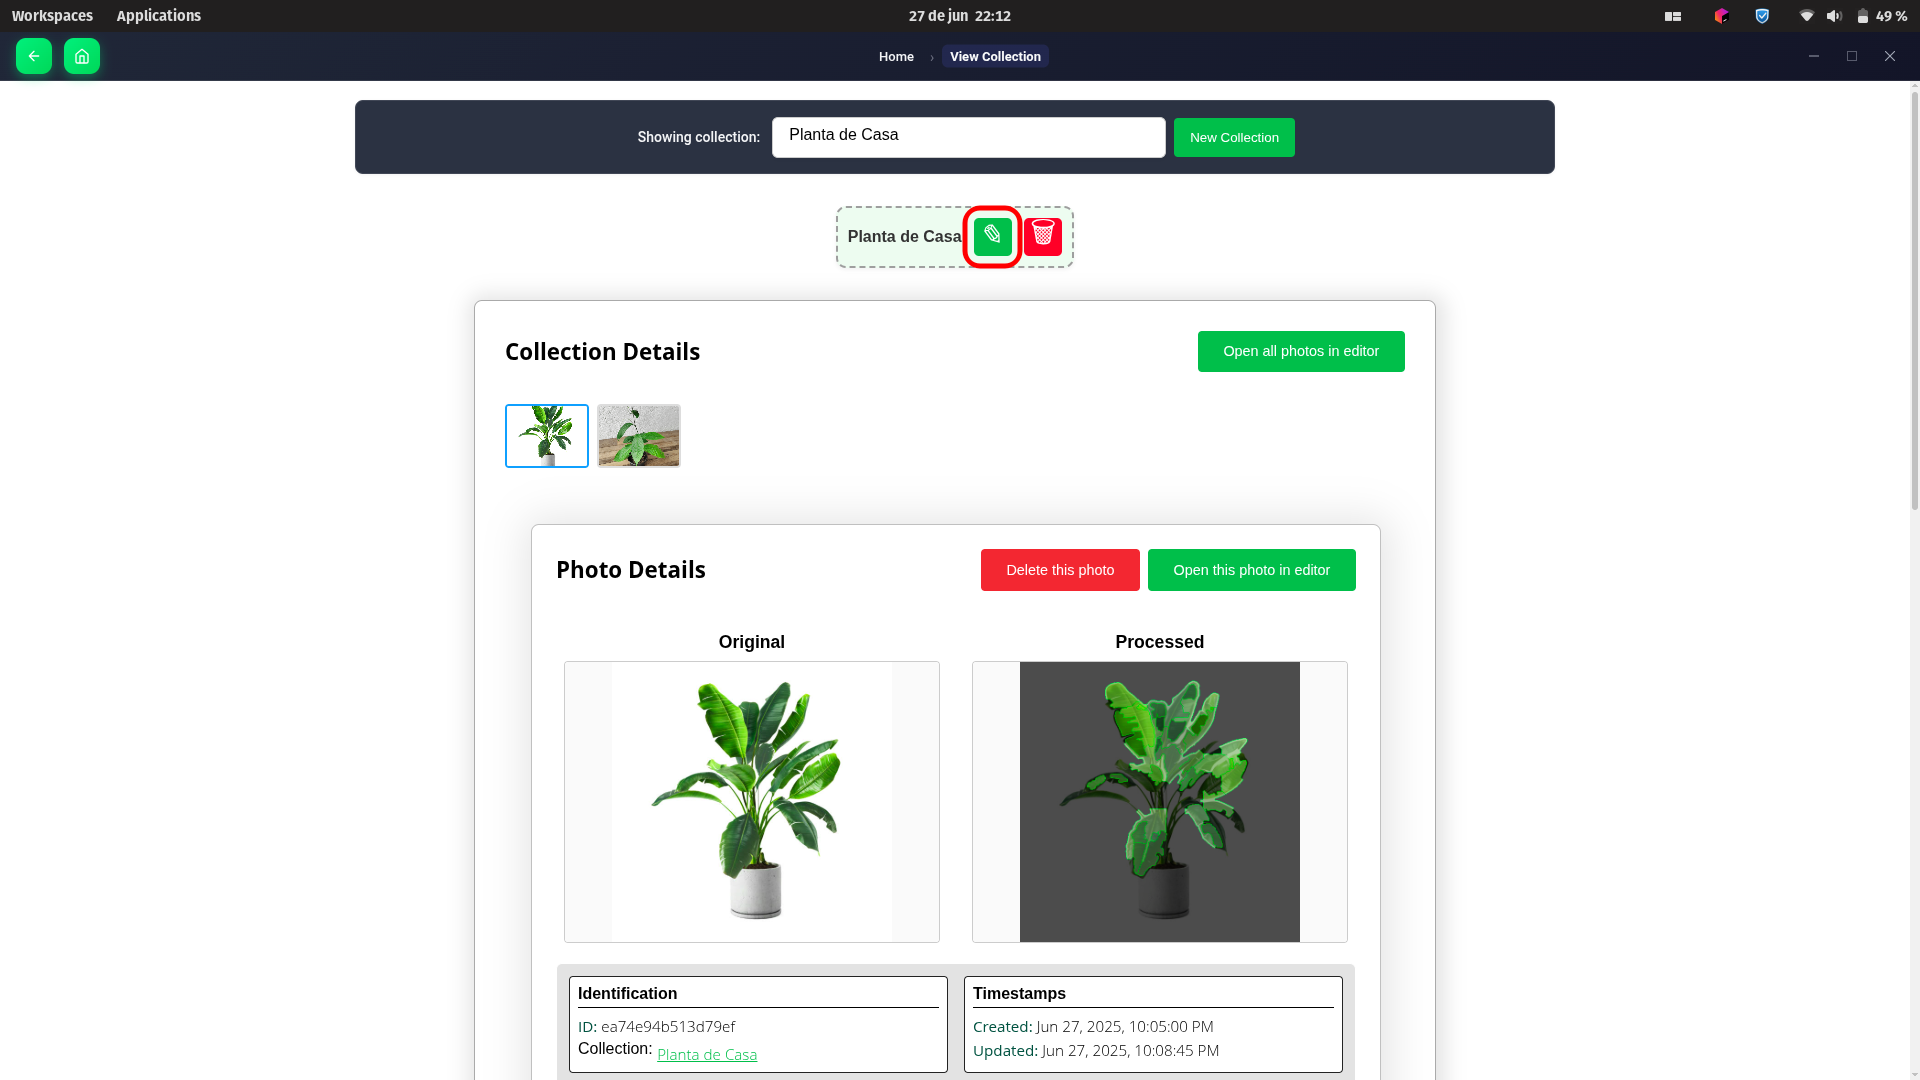
\includegraphics[width=1\textwidth]{../figures/screens/uc008/Screenshot from 2025-06-27 22-12-47.png}
    \caption{Seleção da coleção para renomear. Fonte: os autores}
    \label{fig:uc008-screen2}
\end{figure}

\begin{figure}[H]
    \centering
    \includegraphics[width=1\textwidth]{../figures/screens/uc008/Screenshot from 2025-06-27 22-12-53.png}
    \caption{Edição do nome da coleção. Fonte: os autores}
    \label{fig:uc008-screen3}
\end{figure}

\begin{figure}[H]
    \centering
    \includegraphics[width=1\textwidth]{../figures/screens/uc008/Screenshot from 2025-06-27 22-13-02.png}
    \caption{Confirmação da renomeação. Fonte: os autores}
    \label{fig:uc008-screen4}
\end{figure}

\begin{figure}[H]
    \centering
    \includegraphics[width=1\textwidth]{../figures/screens/uc008/Screenshot from 2025-06-27 22-13-11.png}
    \caption{Coleção renomeada com sucesso. Fonte: os autores}
    \label{fig:uc008-screen5}
\end{figure}

\section{Deletar coleção}

\subsection{HTA Model}

\begin{figure}[H]
    \centering
    \includegraphics[width=0.9\textwidth]{../figures/hta/UC009.png}
    \caption{HTA Model para o caso de uso: Deletar coleção. Fonte: os autores}
    \label{fig:hta-uc009}
\end{figure}

\subsection{Diagrama de Sequência}

\begin{figure}[H]
    \centering
    \includegraphics[width=0.9\textwidth]{../figures/dss/UC009.png}
    \caption{Diagrama de sequência para o caso de uso: Deletar coleção. Fonte: os autores}
    \label{fig:dss-uc009}
\end{figure}

\subsection{Telas da Aplicação}

\begin{figure}[H]
    \centering
    \includegraphics[width=1\textwidth]{../figures/screens/uc009/Screenshot from 2025-06-27 22-13-27.png}
    \caption{Tela inicial para deletar coleção. Fonte: os autores}
    \label{fig:uc009-screen1}
\end{figure}

\begin{figure}[H]
    \centering
    \includegraphics[width=1\textwidth]{../figures/screens/uc009/Screenshot from 2025-06-27 22-13-32.png}
    \caption{Seleção da coleção para deletar. Fonte: os autores}
    \label{fig:uc009-screen2}
\end{figure}

\begin{figure}[H]
    \centering
    \includegraphics[width=1\textwidth]{../figures/screens/uc009/Screenshot from 2025-06-27 22-13-38.png}
    \caption{Confirmação da exclusão. Fonte: os autores}
    \label{fig:uc009-screen3}
\end{figure}

\begin{figure}[H]
    \centering
    \includegraphics[width=1\textwidth]{../figures/screens/uc009/Screenshot from 2025-06-27 22-13-42.png}
    \caption{Coleção deletada com sucesso. Fonte: os autores}
    \label{fig:uc009-screen4}
\end{figure}

\section{Visualizar fotos de coleção}

\subsection{HTA Model}

\begin{figure}[H]
    \centering
    \includegraphics[width=0.9\textwidth]{../figures/hta/UC010.png}
    \caption{HTA Model para o caso de uso: Visualizar fotos de coleção. Fonte: os autores}
    \label{fig:hta-uc010}
\end{figure}

\subsection{Diagrama de Sequência}

\begin{figure}[H]
    \centering
    \includegraphics[width=0.9\textwidth]{../figures/dss/UC010.png}
    \caption{Diagrama de sequência para o caso de uso: Visualizar fotos de coleção. Fonte: os autores}
    \label{fig:dss-uc010}
\end{figure}

\subsection{Telas da Aplicação}

\begin{figure}[H]
    \centering
    \includegraphics[width=1\textwidth]{../figures/screens/uc010/Screenshot from 2025-06-28 17-06-32.png}
    \caption{Tela inicial para visualizar fotos da coleção. Fonte: os autores}
    \label{fig:uc010-screen1}
\end{figure}

\begin{figure}[H]
    \centering
    \includegraphics[width=1\textwidth]{../figures/screens/uc010/Screenshot from 2025-06-28 17-06-44.png}
    \caption{Visualização de todas as fotos dentro da coleção. Fonte: os autores}
    \label{fig:uc010-screen2}
\end{figure}

\begin{figure}[H]
    \centering
    \includegraphics[width=1\textwidth]{../figures/screens/uc010/Screenshot from 2025-06-28 17-07-14.png}
    \caption{Visualização de outras fotos dentro da coleção. Fonte: os autores}
    \label{fig:uc010-screen3}
\end{figure}

\section{Processar foto única}

\subsection{HTA Model}

\begin{figure}[H]
    \centering
    \includegraphics[width=0.9\textwidth]{../figures/hta/UC011.png}
    \caption{HTA Model para o caso de uso: Processar foto única. Fonte: os autores}
    \label{fig:hta-uc011}
\end{figure}

\subsection{Diagrama de Sequência}

\begin{figure}[H]
    \centering
    \includegraphics[width=0.9\textwidth]{../figures/dss/UC011.png}
    \caption{Diagrama de sequência para o caso de uso: Processar foto única. Fonte: os autores}
    \label{fig:dss-uc011}
\end{figure}

\subsection{Telas da Aplicação}

\begin{figure}[H]
    \centering
    \includegraphics[width=1\textwidth]{../figures/screens/uc011/Screenshot from 2025-06-27 22-08-11.png}
    \caption{Seleção da foto para processamento. Fonte: os autores}
    \label{fig:uc011-screen1}
\end{figure}

\begin{figure}[H]
    \centering
    \includegraphics[width=1\textwidth]{../figures/screens/uc011/Screenshot from 2025-06-27 22-08-15.png}
    \caption{Botão de editar fotos. Fonte: os autores}
    \label{fig:uc011-screen2}
\end{figure}

\begin{figure}[H]
    \centering
    \includegraphics[width=1\textwidth]{../figures/screens/uc011/Screenshot from 2025-06-27 22-08-20.png}
    \caption{Seleção dos parâmetros de processamento. Fonte: os autores}
    \label{fig:uc011-screen3}
\end{figure}

\begin{figure}[H]
    \centering
    \includegraphics[width=1\textwidth]{../figures/screens/uc011/Screenshot from 2025-06-27 22-08-42.png}
    \caption{Início do processamento. Fonte: os autores}
    \label{fig:uc011-screen4}
\end{figure}

\begin{figure}[H]
    \centering
    \includegraphics[width=1\textwidth]{../figures/screens/uc011/Screenshot from 2025-06-27 22-08-53.png}
    \caption{Resultado do processamento. Fonte: os autores}
    \label{fig:uc011-screen5}
\end{figure}

\begin{figure}[H]
    \centering
    \includegraphics[width=1\textwidth]{../figures/screens/uc011/Screenshot from 2025-06-27 22-09-06.png}
    \caption{Processamento concluído. Fonte: os autores}
    \label{fig:uc011-screen7}
\end{figure}

\section{Processar múltiplas fotos}

\subsection{HTA Model}

\begin{figure}[H]
    \centering
    \includegraphics[width=0.9\textwidth]{../figures/hta/UC012.png}
    \caption{HTA Model para o caso de uso: Processar múltiplas fotos. Fonte: os autores}
    \label{fig:hta-uc012}
\end{figure}

\subsection{Diagrama de Sequência}

\begin{figure}[H]
    \centering
    \includegraphics[width=0.9\textwidth]{../figures/dss/UC012.png}
    \caption{Diagrama de sequência para o caso de uso: Processar múltiplas fotos. Fonte: os autores}
    \label{fig:dss-uc012}
\end{figure}

\subsection{Telas da Aplicação}

\begin{figure}[H]
    \centering
    \includegraphics[width=1\textwidth]{../figures/screens/uc012/Screenshot from 2025-06-28 16-44-12.png}
    \caption{Seleção da coleção para processamento. Fonte: os autores}
    \label{fig:uc012-screen1}
\end{figure}

\begin{figure}[H]
    \centering
    \includegraphics[width=1\textwidth]{../figures/screens/uc012/Screenshot from 2025-06-28 16-44-15.png}
    \caption{Abertura do editor da coleção (todas as fotos). Fonte: os autores}
    \label{fig:uc012-screen2}
\end{figure}

\begin{figure}[H]
    \centering
    \includegraphics[width=1\textwidth]{../figures/screens/uc012/Screenshot from 2025-06-28 16-44-28.png}
    \caption{Seleção da opção de processar todas as fotos. Fonte: os autores}
    \label{fig:uc012-screen3}
\end{figure}

\begin{figure}[H]
    \centering
    \includegraphics[width=1\textwidth]{../figures/screens/uc012/Screenshot from 2025-06-28 16-44-32.png}
    \caption{Seleção dos parâmetros de processamento. Fonte: os autores}
    \label{fig:uc012-screen4}
\end{figure}

\begin{figure}[H]
    \centering
    \includegraphics[width=1\textwidth]{../figures/screens/uc012/Screenshot from 2025-06-28 16-45-39.png}
    \caption{Início do processamento. Fonte: os autores}
    \label{fig:uc012-screen5}
\end{figure}

\begin{figure}[H]
    \centering
    \includegraphics[width=1\textwidth]{../figures/screens/uc012/Screenshot from 2025-06-28 16-45-48.png}
    \caption{Processamento em andamento. Fonte: os autores}
    \label{fig:uc012-screen6}
\end{figure}

\begin{figure}[H]
    \centering
    \includegraphics[width=1\textwidth]{../figures/screens/uc012/Screenshot from 2025-06-28 16-57-59.png}
    \caption{Visualização do processamento nas imagens. Fonte: os autores}
    \label{fig:uc012-screen7}
\end{figure}

\begin{figure}[H]
    \centering
    \includegraphics[width=1\textwidth]{../figures/screens/uc012/Screenshot from 2025-06-28 16-58-05.png}
    \caption{Confirmar processamento. Fonte: os autores}
    \label{fig:uc012-screen8}
\end{figure}

\begin{figure}[H]
    \centering
    \includegraphics[width=1\textwidth]{../figures/screens/uc012/Screenshot from 2025-06-28 16-58-13.png}
    \caption{Resultado final do processamento múltiplo. Fonte: os autores}
    \label{fig:uc012-screen9}
\end{figure}

\section{Realizar operações de Desfazer/Refazer durante processamento}

\subsection{HTA Model}

\begin{figure}[H]
    \centering
    \includegraphics[width=0.9\textwidth]{../figures/hta/UC013.png}
    \caption{HTA Model para o caso de uso: Desfazer/Refazer durante processamento. Fonte: os autores}
    \label{fig:hta-uc013}
\end{figure}

\subsection{Diagrama de Sequência}

\begin{figure}[H]
    \centering
    \includegraphics[width=0.9\textwidth]{../figures/dss/UC013.png}
    \caption{Diagrama de sequência para o caso de uso: Desfazer/Refazer durante processamento. Fonte: os autores}
    \label{fig:dss-uc013}
\end{figure}

\subsection{Telas da Aplicação}

\begin{figure}[H]
    \centering
    \includegraphics[width=1\textwidth]{../figures/screens/uc013/Screenshot from 2025-06-28 17-11-12.png}
    \caption{Seleção de imagem para processamento. Fonte: os autores}
    \label{fig:uc013-screen1}
\end{figure}

\begin{figure}[H]
    \centering
    \includegraphics[width=1\textwidth]{../figures/screens/uc013/Screenshot from 2025-06-28 17-11-16.png}
    \caption{Início do processamento. Fonte: os autores}
    \label{fig:uc013-screen2}
\end{figure}

\begin{figure}[H]
    \centering
    \includegraphics[width=1\textwidth]{../figures/screens/uc013/Screenshot from 2025-06-28 17-11-19.png}
    \caption{Modificação dos parâmetros do processamento. Fonte: os autores}
    \label{fig:uc013-screen3}
\end{figure}

\begin{figure}[H]
    \centering
    \includegraphics[width=1\textwidth]{../figures/screens/uc013/Screenshot from 2025-06-28 17-11-27.png}
    \caption{Realizar processamento. Fonte: os autores}
    \label{fig:uc013-screen4}
\end{figure}

\begin{figure}[H]
    \centering
    \includegraphics[width=1\textwidth]{../figures/screens/uc013/Screenshot from 2025-06-28 17-11-31.png}
    \caption{Desfazer processamento. Fonte: os autores}
    \label{fig:uc013-screen5}
\end{figure}

\begin{figure}[H]
    \centering
    \includegraphics[width=1\textwidth]{../figures/screens/uc013/Screenshot from 2025-06-28 17-11-36.png}
    \caption{Refazer processamento. Fonte: os autores}
    \label{fig:uc013-screen6}
\end{figure}

\begin{figure}[H]
    \centering
    \includegraphics[width=1\textwidth]{../figures/screens/uc013/Screenshot from 2025-06-28 17-11-39.png}
    \caption{Finalizar processamento. Fonte: os autores}
    \label{fig:uc013-screen7}
\end{figure}

\begin{figure}[H]
    \centering
    \includegraphics[width=1\textwidth]{../figures/screens/uc013/Screenshot from 2025-06-28 17-11-46.png}
    \caption{Resultado final. Fonte: os autores}
    \label{fig:uc013-screen8}
\end{figure}

\section{Visualizar gráficos de crescimento}

\subsection{HTA Model}

\begin{figure}[H]
    \centering
    \includegraphics[width=0.9\textwidth]{../figures/hta/UC014.png}
    \caption{HTA Model para o caso de uso: Visualizar gráficos de crescimento. Fonte: os autores}
    \label{fig:hta-uc014}
\end{figure}

\subsection{Diagrama de Sequência}

\begin{figure}[H]
    \centering
    \includegraphics[width=0.9\textwidth]{../figures/dss/UC014.png}
    \caption{Diagrama de sequência para o caso de uso: Visualizar gráficos de crescimento. Fonte: os autores}
    \label{fig:dss-uc014}
\end{figure}

\subsection{Telas da Aplicação}

\begin{figure}[H]
    \centering
    \includegraphics[width=1\textwidth]{../figures/screens/uc014/Screenshot from 2025-06-28 17-13-06.png}
    \caption{Seleção da coleção para visualizar gráficos. Fonte: os autores}
    \label{fig:uc014-screen2}
\end{figure}

\begin{figure}[H]
    \centering
    \includegraphics[width=1\textwidth]{../figures/screens/uc014/Screenshot from 2025-06-28 17-13-29.png}
    \caption{Coleção selecionada aberta. Fonte: os autores}
    \label{fig:uc014-screen3}
\end{figure}

\begin{figure}[H]
    \centering
    \includegraphics[width=1\textwidth]{../figures/screens/uc014/Screenshot from 2025-06-28 17-13-38.png}
    \caption{Após scroll down, é possível ver os gráficos de evolução da coleção. Fonte: os autores}
    \label{fig:uc014-screen4}
\end{figure}
